\documentclass[twoside]{article}

% Packages required by doxygen
\usepackage{fixltx2e}
\usepackage{calc}
\usepackage{doxygen}
\usepackage[export]{adjustbox} % also loads graphicx
\usepackage{graphicx}
\usepackage[utf8]{inputenc}
\usepackage{makeidx}
\usepackage{multicol}
\usepackage{multirow}
\PassOptionsToPackage{warn}{textcomp}
\usepackage{textcomp}
\usepackage[nointegrals]{wasysym}
\usepackage[table]{xcolor}

% NLS support packages
\usepackage[french]{babel}

% Font selection
\usepackage[T1]{fontenc}
\usepackage[scaled=.90]{helvet}
\usepackage{courier}
\usepackage{amssymb}
\usepackage{sectsty}
\renewcommand{\familydefault}{\sfdefault}
\allsectionsfont{%
  \fontseries{bc}\selectfont%
  \color{darkgray}%
}
\renewcommand{\DoxyLabelFont}{%
  \fontseries{bc}\selectfont%
  \color{darkgray}%
}
\newcommand{\+}{\discretionary{\mbox{\scriptsize$\hookleftarrow$}}{}{}}

% Page & text layout
\usepackage[a4paper]{geometry}
\geometry{vmargin=2cm,hmargin=2cm,lmargin=1.2cm,rmargin=1.2cm}
\tolerance=750
\hfuzz=15pt
\hbadness=750
\setlength{\emergencystretch}{15pt}
\setlength{\parindent}{0cm}
\setlength{\parskip}{3ex plus 2ex minus 2ex}
\makeatletter
\renewcommand{\paragraph}{%
  \@startsection{paragraph}{4}{0ex}{-1.0ex}{1.0ex}{%
    \normalfont\normalsize\bfseries\SS@parafont%
  }%
}
\renewcommand{\subparagraph}{%
  \@startsection{subparagraph}{5}{0ex}{-1.0ex}{1.0ex}{%
    \normalfont\normalsize\bfseries\SS@subparafont%
  }%
}
\makeatother

% Headers & footers
\usepackage{fancyhdr}
\pagestyle{fancyplain}
\fancyhead[LE]{\fancyplain{}{\bfseries\thepage}}
\fancyhead[CE]{\fancyplain{}{}}
\fancyhead[RE]{\fancyplain{}{\bfseries\leftmark}}
\fancyhead[LO]{\fancyplain{}{\bfseries\rightmark}}
\fancyhead[CO]{\fancyplain{}{}}
\fancyhead[RO]{\fancyplain{}{\bfseries\thepage}}
\fancyfoot[LE]{\fancyplain{}{\bfseries\scriptsize TEC}}
\fancyfoot[CE]{\fancyplain{}{}}
\fancyfoot[RE]{\fancyplain{}{\bfseries\scriptsize BTS SN-IR LaSalle Avignon 2019 }}
\fancyfoot[LO]{\fancyplain{}{\bfseries\scriptsize BTS SN-IR LaSalle Avignon 2019 }}
\fancyfoot[CO]{\fancyplain{}{}}
\fancyfoot[RO]{\fancyplain{}{\bfseries\scriptsize TEC}}
\renewcommand{\footrulewidth}{0.4pt}
\renewcommand{\sectionmark}[1]{%
  \markright{\thesection\ #1}%
}

% Indices & bibliography
\usepackage{natbib}
\usepackage[titles]{tocloft}
\setcounter{tocdepth}{3}
\setcounter{secnumdepth}{5}
\makeindex

% Hyperlinks (required, but should be loaded last)
\usepackage{ifpdf}
\ifpdf
  \usepackage[pdftex,pagebackref=true]{hyperref}
\else
  \usepackage[ps2pdf,pagebackref=true]{hyperref}
\fi
\hypersetup{%
  colorlinks=true,%
  linkcolor=blue,%
  citecolor=blue,%
  unicode%
}

% Custom commands
\newcommand{\clearemptydoublepage}{%
  \newpage{\pagestyle{empty}\cleardoublepage}%
}

\usepackage{caption}
\captionsetup{labelsep=space,justification=centering,font={bf},singlelinecheck=off,skip=4pt,position=top}

%===== C O N T E N T S =====

\begin{document}

% Titlepage & ToC
\hypersetup{pageanchor=false,
             bookmarksnumbered=true,
             pdfencoding=unicode
            }
\pagenumbering{alph}
\begin{titlepage}
\vspace*{7cm}
\begin{center}%
{\LARGE Trottinette Électrique Connectée \\[1ex]\large 1.\+1 }\\
\vspace*{1cm}
{\large SY Somphon}\\
\end{center}
\end{titlepage}
\pagenumbering{roman}
\tableofcontents
\pagenumbering{arabic}
\hypersetup{pageanchor=true}

%--- Begin generated contents ---
\section{Le projet T\+EC (Trottinette Électrique Connectée)}
\label{index}\hypertarget{index}{}Système embarqué sur une trottinette électrique équipée de capteurs afin d\textquotesingle{}assister l\textquotesingle{}utilisateur sur son trajet.

\begin{DoxyAuthor}{Auteur}
{\itshape Somphon} SY \href{mailto:somphon.sypro@gmail.com}{\tt somphon.\+sypro@gmail.\+com}
\end{DoxyAuthor}
\hypertarget{index_section_tdm}{}\subsection{Table des matières}\label{index_section_tdm}

\begin{DoxyItemize}
\item \hyperlink{page__r_e_a_d_m_e}{R\+E\+A\+D\+ME}
\item \hyperlink{page_changelog}{Changelog}
\item \hyperlink{page_about}{A propos}
\item \hyperlink{page_licence}{Licence G\+PL} 
\end{DoxyItemize}
\section{Changelog}
\label{page_changelog}
\Hypertarget{page_changelog}
r48 $\vert$ sysom $\vert$ 2019-\/05-\/28 16\+:11\+:41 +0200 (mar. 28 mai 2019) $\vert$ 1 ligne

Ajustement au niveau de l\textquotesingle{}I\+HM , et des interaction entre les boutons / textes

r47 $\vert$ sysom $\vert$ 2019-\/05-\/28 09\+:43\+:36 +0200 (mar. 28 mai 2019) $\vert$ 1 ligne

Ajout d\textquotesingle{}un indicateur de connexion sur la carte ainsi qu\textquotesingle{}un indicateur de batterie sur la carte

r46 $\vert$ sysom $\vert$ 2019-\/05-\/24 11\+:54\+:09 +0200 (ven. 24 mai 2019) $\vert$ 1 ligne

Ajout de l\textquotesingle{}estimation du pourcentage de batterie restante / Modification de l\textquotesingle{}ihm pour l\textquotesingle{}adapté sur un smartphone

r45 $\vert$ sysom $\vert$ 2019-\/05-\/23 16\+:04\+:00 +0200 (jeu. 23 mai 2019) $\vert$ 1 ligne

Ajout des logos liée au données de fonctionnement ainsi qu\textquotesingle{}au choix d\textquotesingle{}itinéraire

r44 $\vert$ sysom $\vert$ 2019-\/05-\/23 15\+:24\+:36 +0200 (jeu. 23 mai 2019) $\vert$ 1 ligne

Ajout de la distance totale entre la position actuelle et la destination

r43 $\vert$ sysom $\vert$ 2019-\/05-\/23 12\+:34\+:11 +0200 (jeu. 23 mai 2019) $\vert$ 1 ligne

Ajout des icones pour les tab button

r42 $\vert$ sysom $\vert$ 2019-\/05-\/23 10\+:30\+:47 +0200 (jeu. 23 mai 2019) $\vert$ 2 lignes

Documentation du code

r41 $\vert$ tvaira $\vert$ 2019-\/05-\/20 11\+:42\+:21 +0200 (lun. 20 mai 2019) $\vert$ 1 ligne

Ajout documentation Doxygen pour tag 0.\+2

r40 $\vert$ tvaira $\vert$ 2019-\/05-\/20 11\+:40\+:11 +0200 (lun. 20 mai 2019) $\vert$ 1 ligne

création du tag 0.\+2

r39 $\vert$ tvaira $\vert$ 2019-\/05-\/20 11\+:38\+:36 +0200 (lun. 20 mai 2019) $\vert$ 1 ligne

Passage des fichiers Doxygen au format Markdown

r38 $\vert$ sysom $\vert$ 2019-\/05-\/09 16\+:52\+:18 +0200 (jeu. 09 mai 2019) $\vert$ 1 ligne

Fix d\textquotesingle{}un bug / Ajout d\textquotesingle{}un qdebug

r37 $\vert$ sysom $\vert$ 2019-\/05-\/05 15\+:37\+:06 +0200 (dim. 05 mai 2019) $\vert$ 1 ligne

Ajout de l\textquotesingle{}arrêt et du reset du timer d\textquotesingle{}utilisation lorsque la tte se déconnecte

r36 $\vert$ sysom $\vert$ 2019-\/05-\/05 15\+:29\+:25 +0200 (dim. 05 mai 2019) $\vert$ 1 ligne

Ajout de la fonctionnalité permettant de savoir la durée d\textquotesingle{}utilisation dès la connexion à la T\+TE

r35 $\vert$ sysom $\vert$ 2019-\/05-\/03 11\+:46\+:04 +0200 (ven. 03 mai 2019) $\vert$ 1 ligne

Modification I\+HM partie Carte

r34 $\vert$ sysom $\vert$ 2019-\/05-\/02 16\+:11\+:47 +0200 (jeu. 02 mai 2019) $\vert$ 1 ligne

Ajout des interactions liée à une déconnexion de la trottinette / Ajout du décodage de la trames / Modification I\+HM

r33 $\vert$ sysom $\vert$ 2019-\/04-\/25 16\+:15\+:03 +0200 (jeu. 25 avril 2019) $\vert$ 1 ligne

Ajout des slot / signaux pour le décodage des trames ainsi que l\textquotesingle{}ajout d\textquotesingle{}une Classe T\+R\+A\+ME qui vas posséder les fonctions responsable du décodage des trames

r32 $\vert$ tvaira $\vert$ 2019-\/04-\/07 06\+:24\+:37 +0200 (dim. 07 avril 2019) $\vert$ 1 ligne

Tag 0.\+1

r31 $\vert$ sysom $\vert$ 2019-\/04-\/06 12\+:03\+:17 +0200 (sam. 06 avril 2019) $\vert$ 1 ligne

Modification Changelog + tag de la première version

r30 $\vert$ sysom $\vert$ 2019-\/04-\/06 11\+:24\+:03 +0200 (sam. 06 avril 2019) $\vert$ 1 ligne

r29 $\vert$ sysom $\vert$ 2019-\/04-\/06 11\+:20\+:14 +0200 (sam. 06 avril 2019) $\vert$ 1 ligne

Mise à jour de la documentation du code

r28 $\vert$ tvaira $\vert$ 2019-\/04-\/05 05\+:29\+:43 +0200 (ven. 05 avril 2019) $\vert$ 1 ligne

Correction commentaires et nom trottinette

r27 $\vert$ tvaira $\vert$ 2019-\/04-\/05 05\+:29\+:33 +0200 (ven. 05 avril 2019) $\vert$ 1 ligne

Correction commentaires et nom trottinette

r26 $\vert$ sysom $\vert$ 2019-\/04-\/03 10\+:44\+:53 +0200 (mer. 03 avril 2019) $\vert$ 1 ligne

Mise à jour de la documentation

r25 $\vert$ tvaira $\vert$ 2019-\/04-\/02 04\+:29\+:03 +0200 (mar. 02 avril 2019) $\vert$ 1 ligne

Validation des commentaires

r24 $\vert$ sysom $\vert$ 2019-\/04-\/01 23\+:19\+:33 +0200 (lun. 01 avril 2019) $\vert$ 1 ligne

Mise à jour de la documentation

r23 $\vert$ tvaira $\vert$ 2019-\/04-\/01 21\+:45\+:15 +0200 (lun. 01 avril 2019) $\vert$ 1 ligne

Controle Qualité Revue 2

r22 $\vert$ sysom $\vert$ 2019-\/04-\/01 18\+:07\+:48 +0200 (lun. 01 avril 2019) $\vert$ 1 ligne

Ajout d\textquotesingle{}un swipeview dans la page Carte

r21 $\vert$ sysom $\vert$ 2019-\/03-\/31 15\+:17\+:38 +0200 (dim. 31 mars 2019) $\vert$ 1 ligne

Ajout de l\textquotesingle{}affichage d\textquotesingle{}un trajet entre la position actuelle et une destination + ajout de l\textquotesingle{}icone destination

r20 $\vert$ sysom $\vert$ 2019-\/03-\/28 16\+:07\+:42 +0100 (jeu. 28 mars 2019) $\vert$ 1 ligne

Ajout du text field pour l\textquotesingle{}adresse de la destination ainsi que du textfield pour la ville de la destination/ modification majeure de la page Carte

r19 $\vert$ sysom $\vert$ 2019-\/03-\/27 10\+:49\+:53 +0100 (mer. 27 mars 2019) $\vert$ 1 ligne

Ajout des fonctions permettant la connection avec un périphérique bluetooth externe utilisant le protocole rfcom + modification de l\textquotesingle{}affichage de l\textquotesingle{}I\+HM lors de la connection

r18 $\vert$ sysom $\vert$ 2019-\/03-\/26 20\+:22\+:12 +0100 (mar. 26 mars 2019) $\vert$ 1 ligne

Ajout d\textquotesingle{}un petit cercle représentant la localisation du téléphone sur la carte ainsi que l\textquotesingle{}ajout de trois bouttons / Zoom + /\+Zoom -\/ Et le boutton qui vas permettre de centrer la carte sur la position de l\textquotesingle{}utilisateur

r17 $\vert$ sysom $\vert$ 2019-\/03-\/21 16\+:21\+:06 +0100 (jeu. 21 mars 2019) $\vert$ 1 ligne

Ajout de l\textquotesingle{}affichage d\textquotesingle{}un périphérique bluetooth externe (nom/adresse M\+AC) , modification de l\textquotesingle{}affichage de l\textquotesingle{}indicateur de chargement en fonction des signaux émis par la Classe Peripherique\+Locale , ajout d\textquotesingle{}un boutton Connexion dans le popup , ajout dans la classe Peripherique\+Locale d\textquotesingle{}accesseur pour le pointeur Trotinette

r16 $\vert$ sysom $\vert$ 2019-\/03-\/21 12\+:12\+:02 +0100 (jeu. 21 mars 2019) $\vert$ 1 ligne

Ajout de la détection de périphérique bluetooth externe

r15 $\vert$ tvaira $\vert$ 2019-\/03-\/20 21\+:03\+:32 +0100 (mer. 20 mars 2019) $\vert$ 2 lignes

Compilation sous Unix/\+Linux

r14 $\vert$ sysom $\vert$ 2019-\/03-\/20 12\+:40\+:05 +0100 (mer. 20 mars 2019) $\vert$ 1 ligne

Ajout méthode Q\+ML / C++ rechercher et arreter , Ajouts des attributs etat\+Connexion , etat\+Recherche , connexion\+Erreur , trotinette\+Detectee ainsi que leur lien avec le fichier Q\+ML , changement du constructeur par défault de la classe Trotinette , changement du constructeur par défaut de la classe Peripherique\+Locale , Modification du switch du Pop\+Pup afin d\textquotesingle{}activer / désactiver la recherche d\textquotesingle{}appareil bluetooth externe via le switch ainsi que l\textquotesingle{}animation de recherche

r13 $\vert$ sysom $\vert$ 2019-\/03-\/20 10\+:45\+:20 +0100 (mer. 20 mars 2019) $\vert$ 1 ligne

Ajout Lib\+Crypto.\+so / libssl.\+so

r12 $\vert$ sysom $\vert$ 2019-\/03-\/20 10\+:43\+:58 +0100 (mer. 20 mars 2019) $\vert$ 1 ligne

Ajout Bibliothéque S\+SL pour android

r11 $\vert$ sysom $\vert$ 2019-\/03-\/20 10\+:39\+:37 +0100 (mer. 20 mars 2019) $\vert$ 1 ligne

Ajout libcrypto.\+so / libssl.\+so dans le dossier android/lib/arm/

r10 $\vert$ tvaira $\vert$ 2019-\/03-\/16 15\+:26\+:16 +0100 (sam. 16 mars 2019) $\vert$ 1 ligne

Notions de classes en Q\+ML (voir Doxygen) et Ajout des bibliothèques S\+SL

r9 $\vert$ tvaira $\vert$ 2019-\/03-\/15 19\+:32\+:17 +0100 (ven. 15 mars 2019) $\vert$ 1 ligne

Modificiation Doxyfile pour Q\+ML

r8 $\vert$ sysom $\vert$ 2019-\/03-\/15 11\+:19\+:12 +0100 (ven. 15 mars 2019) $\vert$ 1 ligne

Mise à jour de la documentation logiciel

r7 $\vert$ sysom $\vert$ 2019-\/03-\/15 11\+:11\+:49 +0100 (ven. 15 mars 2019) $\vert$ 1 ligne

Ajout d\textquotesingle{}un Popup dans la Page 1 et d\textquotesingle{}un Switch / Modification de la taille des bouttons de la Page 1

r6 $\vert$ tvaira $\vert$ 2019-\/03-\/15 06\+:04\+:00 +0100 (ven. 15 mars 2019) $\vert$ 1 ligne

Modificiations documentation du code

r5 $\vert$ sysom $\vert$ 2019-\/03-\/14 15\+:45\+:35 +0100 (jeu. 14 mars 2019) $\vert$ 1 ligne

Début création I\+HM , ajout Tab\+Bar , positionnement de la carte , création des pages Q\+ML

r4 $\vert$ tvaira $\vert$ 2019-\/03-\/14 06\+:46\+:02 +0100 (jeu. 14 mars 2019) $\vert$ 1 ligne

Initialisation commentaires documentation du code

r3 $\vert$ sysom $\vert$ 2019-\/03-\/13 14\+:56\+:45 +0100 (mer. 13 mars 2019) $\vert$ 1 ligne

Création ihm\+Tec + Création classes Peripherique\+Locale et trottinette

r2 $\vert$ tvaira $\vert$ 2019-\/03-\/09 07\+:57\+:58 +0100 (sam. 09 mars 2019) $\vert$ 1 ligne

Initialisation Doxygen

r1 $\vert$ www-\/data $\vert$ 2019-\/02-\/06 20\+:09\+:19 +0100 (mer. 06 févr. 2019) $\vert$ 1 ligne

Creating initial repository structure 
\section{R\+E\+A\+D\+ME}
\label{page__r_e_a_d_m_e}
\Hypertarget{page__r_e_a_d_m_e}
\subsubsection*{Nom \+: T\+EC (\hyperlink{class_trottinette}{Trottinette} Électrique Connectée)}

Système embarqué sur une trottinette électrique équipée de capteurs afin d\textquotesingle{}assister l\textquotesingle{}utilisateur sur son trajet.

\subsubsection*{Numéro de version \+: 1.\+0}

\subsubsection*{Auteur}

\begin{DoxyAuthor}{Auteur}
{\itshape Somphon} SY \href{mailto:somphon.sypro@gmail.com}{\tt somphon.\+sypro@gmail.\+com}
\end{DoxyAuthor}
\subsubsection*{Dépôt S\+VN}

\href{https://svn.riouxsvn.com/tec}{\tt https\+://svn.\+riouxsvn.\+com/tec}

\subsubsection*{Recette IR}


\begin{DoxyItemize}
\item Étudiant 2 \+: Somphon SY
\item Le protocole de communication avec la T\+TE est spécifié et mis en œuvre ;
\item La réception des données de fonctionnement de la T\+TE est effective ;
\item La visualisation des données de fonctionnement de la T\+TE et la durée d\textquotesingle{}utilisation est fonctionelle ;
\item L\textquotesingle{}autonomie pour un parcours est calculée et affichée ;
\item La carte avec la géolocalisation de la T\+TE est affichée et actualisée périodiquement. 
\end{DoxyItemize}
\section{A propos}
\label{page_about}
\Hypertarget{page_about}
\begin{DoxyAuthor}{Auteur}
{\itshape Somphon} SY \href{mailto:somphon.sypro@gmail.com}{\tt somphon.\+sypro@gmail.\+com} 
\end{DoxyAuthor}
\begin{DoxyVersion}{Version}
1.\+0 
\end{DoxyVersion}
\begin{DoxyDate}{Date}
{\bfseries 2019} 
\end{DoxyDate}

\section{Licence G\+PL}
\label{page_licence}
\Hypertarget{page_licence}
This program is free software; you can redistribute it and/or modify it under the terms of the G\+NU General Public License as published by the Free Software Foundation; either version 2 of the License, or (at your option) any later version.

This program is distributed in the hope that it will be useful, but W\+I\+T\+H\+O\+UT A\+NY W\+A\+R\+R\+A\+N\+TY; without even the implied warranty of M\+E\+R\+C\+H\+A\+N\+T\+A\+B\+I\+L\+I\+TY or F\+I\+T\+N\+E\+SS F\+OR A P\+A\+R\+T\+I\+C\+U\+L\+AR P\+U\+R\+P\+O\+SE. See the G\+NU General Public License for more details.

You should have received a copy of the G\+NU General Public License along with this program; if not, write to the Free Software Foundation, Inc., 59 Temple Place, Suite 330, Boston, MA 02111-\/1307 U\+SA 
\section{Documentation des classes}
\hypertarget{class_application}{}\subsection{Référence de la classe Application}
\label{class_application}\index{Application@{Application}}


La fenêtre principale de l\textquotesingle{}application terminal mobile.  




Graphe de collaboration de Application\+:\nopagebreak
\begin{figure}[H]
\begin{center}
\leavevmode
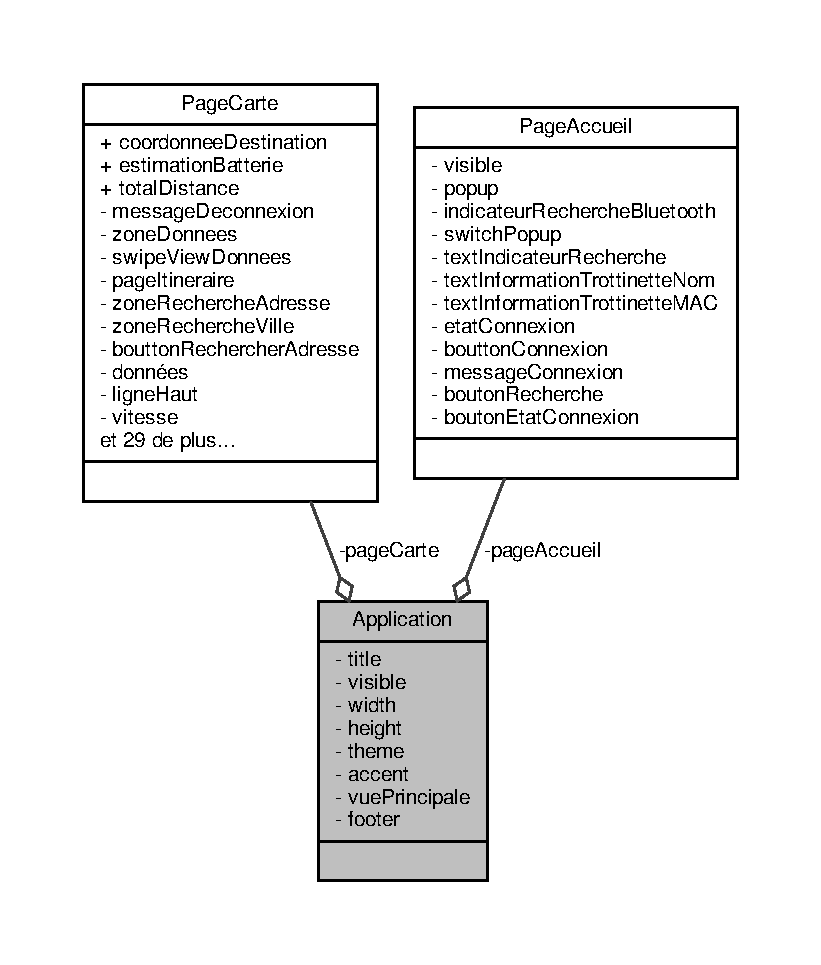
\includegraphics[width=350pt]{class_application__coll__graph}
\end{center}
\end{figure}
\subsubsection*{Attributs privés}
\begin{DoxyCompactItemize}
\item 
var \hyperlink{class_application_a5502df5b638abdf96ab6a995f5a1b942}{title}
\item 
var \hyperlink{class_application_a11dc1b351cae7aca3815fe7c12a8fd30}{visible}
\item 
var \hyperlink{class_application_a4fffe27d37ef2eb5975e18405e1c500b}{width}
\item 
var \hyperlink{class_application_a4f2ad3cef3bc151a8bcccf868a9568ad}{height}
\item 
var Material \hyperlink{class_application_acb2df40484493fb118e57e9dba8aa9d7}{theme}
\item 
var Material \hyperlink{class_application_a97c99a04ac1a1364a3118596f90e95e3}{accent}
\item 
Swipe\+View \hyperlink{class_application_aa725ab76431c16db88823ae84d69268d}{vue\+Principale}
\item 
\hyperlink{class_page_accueil}{Page\+Accueil} \hyperlink{class_application_a226e1b6b8d71ee2716386de3b99dc847}{page\+Accueil}
\item 
\hyperlink{class_page_carte}{Page\+Carte} \hyperlink{class_application_a6e982ff7788a5196389702b5cdc45e41}{page\+Carte}
\item 
var \hyperlink{class_application_ab1ae6209562017c3a95b47108cb5af6b}{footer}
\end{DoxyCompactItemize}


\subsubsection{Description détaillée}
\begin{DoxyAuthor}{Auteur}
Somphon Sy
\end{DoxyAuthor}
\begin{DoxyVersion}{Version}
1.\+1 
\end{DoxyVersion}


\subsubsection{Documentation des données membres}
\mbox{\Hypertarget{class_application_a97c99a04ac1a1364a3118596f90e95e3}\label{class_application_a97c99a04ac1a1364a3118596f90e95e3}} 
\index{Application@{Application}!accent@{accent}}
\index{accent@{accent}!Application@{Application}}
\paragraph{\texorpdfstring{accent}{accent}}
{\footnotesize\ttfamily var Material Application\+::accent\hspace{0.3cm}{\ttfamily [private]}}

\mbox{\Hypertarget{class_application_ab1ae6209562017c3a95b47108cb5af6b}\label{class_application_ab1ae6209562017c3a95b47108cb5af6b}} 
\index{Application@{Application}!footer@{footer}}
\index{footer@{footer}!Application@{Application}}
\paragraph{\texorpdfstring{footer}{footer}}
{\footnotesize\ttfamily var Application\+::footer\hspace{0.3cm}{\ttfamily [private]}}

\mbox{\Hypertarget{class_application_a4f2ad3cef3bc151a8bcccf868a9568ad}\label{class_application_a4f2ad3cef3bc151a8bcccf868a9568ad}} 
\index{Application@{Application}!height@{height}}
\index{height@{height}!Application@{Application}}
\paragraph{\texorpdfstring{height}{height}}
{\footnotesize\ttfamily var Application\+::height\hspace{0.3cm}{\ttfamily [private]}}

\mbox{\Hypertarget{class_application_a226e1b6b8d71ee2716386de3b99dc847}\label{class_application_a226e1b6b8d71ee2716386de3b99dc847}} 
\index{Application@{Application}!page\+Accueil@{page\+Accueil}}
\index{page\+Accueil@{page\+Accueil}!Application@{Application}}
\paragraph{\texorpdfstring{page\+Accueil}{pageAccueil}}
{\footnotesize\ttfamily \hyperlink{class_page_accueil}{Page\+Accueil} Application\+::page\+Accueil\hspace{0.3cm}{\ttfamily [private]}}

\mbox{\Hypertarget{class_application_a6e982ff7788a5196389702b5cdc45e41}\label{class_application_a6e982ff7788a5196389702b5cdc45e41}} 
\index{Application@{Application}!page\+Carte@{page\+Carte}}
\index{page\+Carte@{page\+Carte}!Application@{Application}}
\paragraph{\texorpdfstring{page\+Carte}{pageCarte}}
{\footnotesize\ttfamily \hyperlink{class_page_carte}{Page\+Carte} Application\+::page\+Carte\hspace{0.3cm}{\ttfamily [private]}}

\mbox{\Hypertarget{class_application_acb2df40484493fb118e57e9dba8aa9d7}\label{class_application_acb2df40484493fb118e57e9dba8aa9d7}} 
\index{Application@{Application}!theme@{theme}}
\index{theme@{theme}!Application@{Application}}
\paragraph{\texorpdfstring{theme}{theme}}
{\footnotesize\ttfamily var Material Application\+::theme\hspace{0.3cm}{\ttfamily [private]}}

\mbox{\Hypertarget{class_application_a5502df5b638abdf96ab6a995f5a1b942}\label{class_application_a5502df5b638abdf96ab6a995f5a1b942}} 
\index{Application@{Application}!title@{title}}
\index{title@{title}!Application@{Application}}
\paragraph{\texorpdfstring{title}{title}}
{\footnotesize\ttfamily var Application\+::title\hspace{0.3cm}{\ttfamily [private]}}

\mbox{\Hypertarget{class_application_a11dc1b351cae7aca3815fe7c12a8fd30}\label{class_application_a11dc1b351cae7aca3815fe7c12a8fd30}} 
\index{Application@{Application}!visible@{visible}}
\index{visible@{visible}!Application@{Application}}
\paragraph{\texorpdfstring{visible}{visible}}
{\footnotesize\ttfamily var Application\+::visible\hspace{0.3cm}{\ttfamily [private]}}

\mbox{\Hypertarget{class_application_aa725ab76431c16db88823ae84d69268d}\label{class_application_aa725ab76431c16db88823ae84d69268d}} 
\index{Application@{Application}!vue\+Principale@{vue\+Principale}}
\index{vue\+Principale@{vue\+Principale}!Application@{Application}}
\paragraph{\texorpdfstring{vue\+Principale}{vuePrincipale}}
{\footnotesize\ttfamily Swipe\+View Application\+::vue\+Principale\hspace{0.3cm}{\ttfamily [private]}}

\mbox{\Hypertarget{class_application_a4fffe27d37ef2eb5975e18405e1c500b}\label{class_application_a4fffe27d37ef2eb5975e18405e1c500b}} 
\index{Application@{Application}!width@{width}}
\index{width@{width}!Application@{Application}}
\paragraph{\texorpdfstring{width}{width}}
{\footnotesize\ttfamily var Application\+::width\hspace{0.3cm}{\ttfamily [private]}}



La documentation de cette classe a été générée à partir du fichier suivant \+:\begin{DoxyCompactItemize}
\item 
\hyperlink{_application_8qml}{Application.\+qml}\end{DoxyCompactItemize}

\hypertarget{class_chronometre_utilisation}{}\subsection{Référence de la classe Chronometre\+Utilisation}
\label{class_chronometre_utilisation}\index{Chronometre\+Utilisation@{Chronometre\+Utilisation}}


Déclaration de la classe \hyperlink{class_chronometre_utilisation}{Chronometre\+Utilisation}.  




{\ttfamily \#include $<$chronometreutilisation.\+h$>$}



Graphe de collaboration de Chronometre\+Utilisation\+:\nopagebreak
\begin{figure}[H]
\begin{center}
\leavevmode
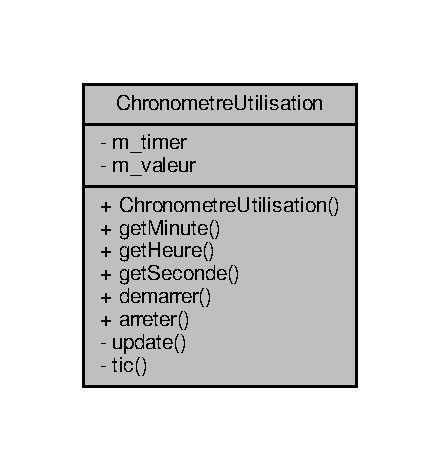
\includegraphics[width=211pt]{class_chronometre_utilisation__coll__graph}
\end{center}
\end{figure}
\subsubsection*{Connecteurs publics}
\begin{DoxyCompactItemize}
\item 
void \hyperlink{class_chronometre_utilisation_ac3f2fb837e9ba408d4dcaf488b289c64}{demarrer} (int top=\hyperlink{chronometreutilisation_8h_ad0750d12e2f5f404ec458d4066a53fa4}{P\+E\+R\+I\+O\+DE})
\begin{DoxyCompactList}\small\item\em Slot lançant le timer du chrono. \end{DoxyCompactList}\item 
void \hyperlink{class_chronometre_utilisation_a938c4c86a6b33eaf60af7be81ee7ec32}{arreter} ()
\begin{DoxyCompactList}\small\item\em Slot arrêtant le timer du chrono. \end{DoxyCompactList}\end{DoxyCompactItemize}
\subsubsection*{Signaux}
\begin{DoxyCompactItemize}
\item 
void \hyperlink{class_chronometre_utilisation_ae4e197f888e33feb23801d2edcf2c4a5}{chrono\+Updated} (Q\+String)
\begin{DoxyCompactList}\small\item\em Signal contenant la variable contenant l\textquotesingle{}heure. \end{DoxyCompactList}\end{DoxyCompactItemize}
\subsubsection*{Fonctions membres publiques}
\begin{DoxyCompactItemize}
\item 
\hyperlink{class_chronometre_utilisation_a499bd70e5056ddb71df022848d1e345e}{Chronometre\+Utilisation} (Q\+Object $\ast$parent=nullptr)
\begin{DoxyCompactList}\small\item\em Constructeur de la classe \hyperlink{class_chronometre_utilisation}{Chronometre\+Utilisation}. \end{DoxyCompactList}\item 
long \hyperlink{class_chronometre_utilisation_a2c137076fcda83a14a5bad01b915196f}{get\+Minute} ()
\begin{DoxyCompactList}\small\item\em Retourne les minutes du chrono. \end{DoxyCompactList}\item 
long \hyperlink{class_chronometre_utilisation_a03c732560e07a2014129a7da8bb2307b}{get\+Heure} ()
\begin{DoxyCompactList}\small\item\em Retourne l\textquotesingle{}heure du chrono. \end{DoxyCompactList}\item 
long \hyperlink{class_chronometre_utilisation_a62dde8f710b8e015ba6124e8b44fe2da}{get\+Seconde} ()
\begin{DoxyCompactList}\small\item\em Retourne les secondes du chrono. \end{DoxyCompactList}\end{DoxyCompactItemize}
\subsubsection*{Connecteurs privés}
\begin{DoxyCompactItemize}
\item 
void \hyperlink{class_chronometre_utilisation_ab8dc7eb855ec9e24daefa4e185051d2e}{tic} ()
\begin{DoxyCompactList}\small\item\em Slot qui incrémente le timer du chrono. \end{DoxyCompactList}\end{DoxyCompactItemize}
\subsubsection*{Fonctions membres privées}
\begin{DoxyCompactItemize}
\item 
void \hyperlink{class_chronometre_utilisation_add760c3052342baec482fe0752a89b86}{update} ()
\begin{DoxyCompactList}\small\item\em Met à jour la variable contenant l\textquotesingle{}heure. \end{DoxyCompactList}\end{DoxyCompactItemize}
\subsubsection*{Attributs privés}
\begin{DoxyCompactItemize}
\item 
Q\+Timer $\ast$ \hyperlink{class_chronometre_utilisation_ae86620ca7d91c0d06c2e695493638bf2}{m\+\_\+timer}
\begin{DoxyCompactList}\small\item\em Pointeur sur une classe Q\+Timer. \end{DoxyCompactList}\item 
long \hyperlink{class_chronometre_utilisation_a7ef8b30ae4b6db56b9be832c847186ea}{m\+\_\+valeur}
\begin{DoxyCompactList}\small\item\em Compteur de l\textquotesingle{}horloge. \end{DoxyCompactList}\end{DoxyCompactItemize}


\subsubsection{Description détaillée}
\begin{DoxyAuthor}{Auteur}
Somphon Sy
\end{DoxyAuthor}
\begin{DoxyVersion}{Version}
1.\+1 
\end{DoxyVersion}


\subsubsection{Documentation des constructeurs et destructeur}
\mbox{\Hypertarget{class_chronometre_utilisation_a499bd70e5056ddb71df022848d1e345e}\label{class_chronometre_utilisation_a499bd70e5056ddb71df022848d1e345e}} 
\index{Chronometre\+Utilisation@{Chronometre\+Utilisation}!Chronometre\+Utilisation@{Chronometre\+Utilisation}}
\index{Chronometre\+Utilisation@{Chronometre\+Utilisation}!Chronometre\+Utilisation@{Chronometre\+Utilisation}}
\paragraph{\texorpdfstring{Chronometre\+Utilisation()}{ChronometreUtilisation()}}
{\footnotesize\ttfamily Chronometre\+Utilisation\+::\+Chronometre\+Utilisation (\begin{DoxyParamCaption}\item[{Q\+Object $\ast$}]{parent = {\ttfamily nullptr} }\end{DoxyParamCaption})\hspace{0.3cm}{\ttfamily [explicit]}}


\begin{DoxyParams}{Paramètres}
{\em parent} & Q\+Object Adresse de l\textquotesingle{}objet Qt parent \\
\hline
\end{DoxyParams}


Références \hyperlink{class_chronometre_utilisation_ae86620ca7d91c0d06c2e695493638bf2}{m\+\_\+timer}, \hyperlink{class_chronometre_utilisation_a7ef8b30ae4b6db56b9be832c847186ea}{m\+\_\+valeur}, et \hyperlink{class_chronometre_utilisation_ab8dc7eb855ec9e24daefa4e185051d2e}{tic()}.


\begin{DoxyCode}
00024                                                               : QObject(parent)
00025 \{
00026     \textcolor{comment}{// initialise la valeur du compteur de tic d'horloge}
00027     \hyperlink{class_chronometre_utilisation_a7ef8b30ae4b6db56b9be832c847186ea}{m\_valeur} = 0;
00028 
00029     \textcolor{comment}{// instancie le timer (base de temps) de l'horloge}
00030     \hyperlink{class_chronometre_utilisation_ae86620ca7d91c0d06c2e695493638bf2}{m\_timer} = \textcolor{keyword}{new} QTimer(\textcolor{keyword}{this});
00031 
00032     \textcolor{comment}{// connecte le signal d'expiration (timeout) d'une période (top d'horloge) au slot tic()}
00033     connect(\hyperlink{class_chronometre_utilisation_ae86620ca7d91c0d06c2e695493638bf2}{m\_timer}, SIGNAL(timeout()), \textcolor{keyword}{this}, SLOT(\hyperlink{class_chronometre_utilisation_ab8dc7eb855ec9e24daefa4e185051d2e}{tic}()));
00034 \}
\end{DoxyCode}


\subsubsection{Documentation des fonctions membres}
\mbox{\Hypertarget{class_chronometre_utilisation_a938c4c86a6b33eaf60af7be81ee7ec32}\label{class_chronometre_utilisation_a938c4c86a6b33eaf60af7be81ee7ec32}} 
\index{Chronometre\+Utilisation@{Chronometre\+Utilisation}!arreter@{arreter}}
\index{arreter@{arreter}!Chronometre\+Utilisation@{Chronometre\+Utilisation}}
\paragraph{\texorpdfstring{arreter}{arreter}}
{\footnotesize\ttfamily void Chronometre\+Utilisation\+::arreter (\begin{DoxyParamCaption}{ }\end{DoxyParamCaption})\hspace{0.3cm}{\ttfamily [slot]}}



Références \hyperlink{class_chronometre_utilisation_ae86620ca7d91c0d06c2e695493638bf2}{m\+\_\+timer}, \hyperlink{class_chronometre_utilisation_a7ef8b30ae4b6db56b9be832c847186ea}{m\+\_\+valeur}, et \hyperlink{class_chronometre_utilisation_add760c3052342baec482fe0752a89b86}{update()}.


\begin{DoxyCode}
00139 \{
00140     \hyperlink{class_chronometre_utilisation_a7ef8b30ae4b6db56b9be832c847186ea}{m\_valeur} = 0 ;
00141     \hyperlink{class_chronometre_utilisation_ae86620ca7d91c0d06c2e695493638bf2}{m\_timer}->stop();
00142     \hyperlink{class_chronometre_utilisation_add760c3052342baec482fe0752a89b86}{update}();
00143     qDebug() << \textcolor{stringliteral}{"ChronometreUtilisation::arreter()"};
00144 \}
\end{DoxyCode}
\mbox{\Hypertarget{class_chronometre_utilisation_ae4e197f888e33feb23801d2edcf2c4a5}\label{class_chronometre_utilisation_ae4e197f888e33feb23801d2edcf2c4a5}} 
\index{Chronometre\+Utilisation@{Chronometre\+Utilisation}!chrono\+Updated@{chrono\+Updated}}
\index{chrono\+Updated@{chrono\+Updated}!Chronometre\+Utilisation@{Chronometre\+Utilisation}}
\paragraph{\texorpdfstring{chrono\+Updated}{chronoUpdated}}
{\footnotesize\ttfamily void Chronometre\+Utilisation\+::chrono\+Updated (\begin{DoxyParamCaption}\item[{Q\+String}]{ }\end{DoxyParamCaption})\hspace{0.3cm}{\ttfamily [signal]}}



Référencé par \hyperlink{class_chronometre_utilisation_add760c3052342baec482fe0752a89b86}{update()}.

\mbox{\Hypertarget{class_chronometre_utilisation_ac3f2fb837e9ba408d4dcaf488b289c64}\label{class_chronometre_utilisation_ac3f2fb837e9ba408d4dcaf488b289c64}} 
\index{Chronometre\+Utilisation@{Chronometre\+Utilisation}!demarrer@{demarrer}}
\index{demarrer@{demarrer}!Chronometre\+Utilisation@{Chronometre\+Utilisation}}
\paragraph{\texorpdfstring{demarrer}{demarrer}}
{\footnotesize\ttfamily Chronometre\+Utilisation\+::demarrer (\begin{DoxyParamCaption}\item[{int}]{top = {\ttfamily \hyperlink{chronometreutilisation_8h_ad0750d12e2f5f404ec458d4066a53fa4}{P\+E\+R\+I\+O\+DE}} }\end{DoxyParamCaption})\hspace{0.3cm}{\ttfamily [slot]}}

Arrête le chronomètre.

Démarre le chronomètre. 

Références \hyperlink{class_chronometre_utilisation_ae86620ca7d91c0d06c2e695493638bf2}{m\+\_\+timer}.


\begin{DoxyCode}
00128 \{
00129     qDebug() << \textcolor{stringliteral}{"ChronometreUtilisation::demarrer()"};
00130     \hyperlink{class_chronometre_utilisation_ae86620ca7d91c0d06c2e695493638bf2}{m\_timer}->start(top);
00131 \}
\end{DoxyCode}
\mbox{\Hypertarget{class_chronometre_utilisation_a03c732560e07a2014129a7da8bb2307b}\label{class_chronometre_utilisation_a03c732560e07a2014129a7da8bb2307b}} 
\index{Chronometre\+Utilisation@{Chronometre\+Utilisation}!get\+Heure@{get\+Heure}}
\index{get\+Heure@{get\+Heure}!Chronometre\+Utilisation@{Chronometre\+Utilisation}}
\paragraph{\texorpdfstring{get\+Heure()}{getHeure()}}
{\footnotesize\ttfamily long Chronometre\+Utilisation\+::get\+Heure (\begin{DoxyParamCaption}{ }\end{DoxyParamCaption})}

Accesseur des heures du chrono.

\begin{DoxyReturn}{Renvoie}
long heure du chronomètre 
\end{DoxyReturn}


Références \hyperlink{class_chronometre_utilisation_a7ef8b30ae4b6db56b9be832c847186ea}{m\+\_\+valeur}.



Référencé par \hyperlink{class_chronometre_utilisation_add760c3052342baec482fe0752a89b86}{update()}.


\begin{DoxyCode}
00058 \{
00059     \textcolor{keywordtype}{long} heure = \hyperlink{class_chronometre_utilisation_a7ef8b30ae4b6db56b9be832c847186ea}{m\_valeur}/36000 ;
00060     \textcolor{keywordflow}{if} (heure >= 24)
00061     \{
00062         heure -= 24;
00063         \textcolor{keywordflow}{return} heure;
00064     \}
00065     \textcolor{keywordflow}{else}
00066     \textcolor{keywordflow}{return} heure;
00067 \}
\end{DoxyCode}
\mbox{\Hypertarget{class_chronometre_utilisation_a2c137076fcda83a14a5bad01b915196f}\label{class_chronometre_utilisation_a2c137076fcda83a14a5bad01b915196f}} 
\index{Chronometre\+Utilisation@{Chronometre\+Utilisation}!get\+Minute@{get\+Minute}}
\index{get\+Minute@{get\+Minute}!Chronometre\+Utilisation@{Chronometre\+Utilisation}}
\paragraph{\texorpdfstring{get\+Minute()}{getMinute()}}
{\footnotesize\ttfamily long Chronometre\+Utilisation\+::get\+Minute (\begin{DoxyParamCaption}{ }\end{DoxyParamCaption})}

Accesseur des minutes du chrono.

\begin{DoxyReturn}{Renvoie}
long minute du chronomètre 
\end{DoxyReturn}


Références \hyperlink{class_chronometre_utilisation_a7ef8b30ae4b6db56b9be832c847186ea}{m\+\_\+valeur}.



Référencé par \hyperlink{class_chronometre_utilisation_add760c3052342baec482fe0752a89b86}{update()}.


\begin{DoxyCode}
00045 \{
00046     \textcolor{keywordflow}{return} (\hyperlink{class_chronometre_utilisation_a7ef8b30ae4b6db56b9be832c847186ea}{m\_valeur}%36000)/600;
00047 \}
\end{DoxyCode}
\mbox{\Hypertarget{class_chronometre_utilisation_a62dde8f710b8e015ba6124e8b44fe2da}\label{class_chronometre_utilisation_a62dde8f710b8e015ba6124e8b44fe2da}} 
\index{Chronometre\+Utilisation@{Chronometre\+Utilisation}!get\+Seconde@{get\+Seconde}}
\index{get\+Seconde@{get\+Seconde}!Chronometre\+Utilisation@{Chronometre\+Utilisation}}
\paragraph{\texorpdfstring{get\+Seconde()}{getSeconde()}}
{\footnotesize\ttfamily long Chronometre\+Utilisation\+::get\+Seconde (\begin{DoxyParamCaption}{ }\end{DoxyParamCaption})}

Accesseur des secondes du chrono.

\begin{DoxyReturn}{Renvoie}
long secondes du chronomètre 
\end{DoxyReturn}


Références \hyperlink{class_chronometre_utilisation_a7ef8b30ae4b6db56b9be832c847186ea}{m\+\_\+valeur}.



Référencé par \hyperlink{class_chronometre_utilisation_add760c3052342baec482fe0752a89b86}{update()}.


\begin{DoxyCode}
00077 \{
00078      \textcolor{keywordflow}{return} ((\hyperlink{class_chronometre_utilisation_a7ef8b30ae4b6db56b9be832c847186ea}{m\_valeur}/10)%60);
00079 \}
\end{DoxyCode}
\mbox{\Hypertarget{class_chronometre_utilisation_ab8dc7eb855ec9e24daefa4e185051d2e}\label{class_chronometre_utilisation_ab8dc7eb855ec9e24daefa4e185051d2e}} 
\index{Chronometre\+Utilisation@{Chronometre\+Utilisation}!tic@{tic}}
\index{tic@{tic}!Chronometre\+Utilisation@{Chronometre\+Utilisation}}
\paragraph{\texorpdfstring{tic}{tic}}
{\footnotesize\ttfamily void Chronometre\+Utilisation\+::tic (\begin{DoxyParamCaption}{ }\end{DoxyParamCaption})\hspace{0.3cm}{\ttfamily [private]}, {\ttfamily [slot]}}

Incrémente la variable contenant le temps du chronomètre. 

Références \hyperlink{class_chronometre_utilisation_a7ef8b30ae4b6db56b9be832c847186ea}{m\+\_\+valeur}, et \hyperlink{class_chronometre_utilisation_add760c3052342baec482fe0752a89b86}{update()}.



Référencé par \hyperlink{class_chronometre_utilisation_a499bd70e5056ddb71df022848d1e345e}{Chronometre\+Utilisation()}.


\begin{DoxyCode}
00115 \{
00116     \textcolor{comment}{// incrémente le compteur de top d'horloge}
00117     \hyperlink{class_chronometre_utilisation_a7ef8b30ae4b6db56b9be832c847186ea}{m\_valeur}++;
00118     \textcolor{comment}{// demande la mise à jour l'affichage de l'horloge}
00119     \hyperlink{class_chronometre_utilisation_add760c3052342baec482fe0752a89b86}{update}();
00120 \}
\end{DoxyCode}
\mbox{\Hypertarget{class_chronometre_utilisation_add760c3052342baec482fe0752a89b86}\label{class_chronometre_utilisation_add760c3052342baec482fe0752a89b86}} 
\index{Chronometre\+Utilisation@{Chronometre\+Utilisation}!update@{update}}
\index{update@{update}!Chronometre\+Utilisation@{Chronometre\+Utilisation}}
\paragraph{\texorpdfstring{update()}{update()}}
{\footnotesize\ttfamily void Chronometre\+Utilisation\+::update (\begin{DoxyParamCaption}{ }\end{DoxyParamCaption})\hspace{0.3cm}{\ttfamily [private]}}

Met à jour la variable contenant la durée du temps d\textquotesingle{}utilisation. 

Références \hyperlink{class_chronometre_utilisation_ae4e197f888e33feb23801d2edcf2c4a5}{chrono\+Updated()}, \hyperlink{class_chronometre_utilisation_a03c732560e07a2014129a7da8bb2307b}{get\+Heure()}, \hyperlink{class_chronometre_utilisation_a2c137076fcda83a14a5bad01b915196f}{get\+Minute()}, et \hyperlink{class_chronometre_utilisation_a62dde8f710b8e015ba6124e8b44fe2da}{get\+Seconde()}.



Référencé par \hyperlink{class_chronometre_utilisation_a938c4c86a6b33eaf60af7be81ee7ec32}{arreter()}, et \hyperlink{class_chronometre_utilisation_ab8dc7eb855ec9e24daefa4e185051d2e}{tic()}.


\begin{DoxyCode}
00088 \{
00089    QString heure, minute , seconde , msec;
00090 
00091    \textcolor{comment}{// met à jour l'affichage de l'horloge}
00092    \textcolor{keywordflow}{if} (\hyperlink{class_chronometre_utilisation_a03c732560e07a2014129a7da8bb2307b}{getHeure}() < 10)
00093       heure = \textcolor{stringliteral}{"0"} + QString::number(\hyperlink{class_chronometre_utilisation_a03c732560e07a2014129a7da8bb2307b}{getHeure}());
00094    \textcolor{keywordflow}{else} heure = QString::number(\hyperlink{class_chronometre_utilisation_a03c732560e07a2014129a7da8bb2307b}{getHeure}());
00095    \textcolor{keywordflow}{if} (\hyperlink{class_chronometre_utilisation_a2c137076fcda83a14a5bad01b915196f}{getMinute}() < 10)
00096       minute = \textcolor{stringliteral}{"0"} + QString::number(\hyperlink{class_chronometre_utilisation_a2c137076fcda83a14a5bad01b915196f}{getMinute}());
00097    \textcolor{keywordflow}{else} minute = QString::number(\hyperlink{class_chronometre_utilisation_a2c137076fcda83a14a5bad01b915196f}{getMinute}());
00098    \textcolor{keywordflow}{if} (\hyperlink{class_chronometre_utilisation_a62dde8f710b8e015ba6124e8b44fe2da}{getSeconde}() < 10 )
00099        seconde = \textcolor{stringliteral}{"0"} + QString::number(\hyperlink{class_chronometre_utilisation_a62dde8f710b8e015ba6124e8b44fe2da}{getSeconde}());
00100    \textcolor{keywordflow}{else} seconde = QString::number(\hyperlink{class_chronometre_utilisation_a62dde8f710b8e015ba6124e8b44fe2da}{getSeconde}());
00101    \textcolor{keywordflow}{if} (\hyperlink{class_chronometre_utilisation_a62dde8f710b8e015ba6124e8b44fe2da}{getSeconde}() < 10 )
00102        seconde = \textcolor{stringliteral}{"0"} + QString::number(\hyperlink{class_chronometre_utilisation_a62dde8f710b8e015ba6124e8b44fe2da}{getSeconde}());
00103    \textcolor{keywordflow}{else} seconde = QString::number(\hyperlink{class_chronometre_utilisation_a62dde8f710b8e015ba6124e8b44fe2da}{getSeconde}());
00104 
00105    QString text = heure + \textcolor{stringliteral}{":"} + minute + \textcolor{stringliteral}{":"} + seconde  ;
00106    emit \hyperlink{class_chronometre_utilisation_ae4e197f888e33feb23801d2edcf2c4a5}{chronoUpdated}(text);
00107 \}
\end{DoxyCode}


\subsubsection{Documentation des données membres}
\mbox{\Hypertarget{class_chronometre_utilisation_ae86620ca7d91c0d06c2e695493638bf2}\label{class_chronometre_utilisation_ae86620ca7d91c0d06c2e695493638bf2}} 
\index{Chronometre\+Utilisation@{Chronometre\+Utilisation}!m\+\_\+timer@{m\+\_\+timer}}
\index{m\+\_\+timer@{m\+\_\+timer}!Chronometre\+Utilisation@{Chronometre\+Utilisation}}
\paragraph{\texorpdfstring{m\+\_\+timer}{m\_timer}}
{\footnotesize\ttfamily Q\+Timer$\ast$ Chronometre\+Utilisation\+::m\+\_\+timer\hspace{0.3cm}{\ttfamily [private]}}



Référencé par \hyperlink{class_chronometre_utilisation_a938c4c86a6b33eaf60af7be81ee7ec32}{arreter()}, \hyperlink{class_chronometre_utilisation_a499bd70e5056ddb71df022848d1e345e}{Chronometre\+Utilisation()}, et \hyperlink{class_chronometre_utilisation_ac3f2fb837e9ba408d4dcaf488b289c64}{demarrer()}.

\mbox{\Hypertarget{class_chronometre_utilisation_a7ef8b30ae4b6db56b9be832c847186ea}\label{class_chronometre_utilisation_a7ef8b30ae4b6db56b9be832c847186ea}} 
\index{Chronometre\+Utilisation@{Chronometre\+Utilisation}!m\+\_\+valeur@{m\+\_\+valeur}}
\index{m\+\_\+valeur@{m\+\_\+valeur}!Chronometre\+Utilisation@{Chronometre\+Utilisation}}
\paragraph{\texorpdfstring{m\+\_\+valeur}{m\_valeur}}
{\footnotesize\ttfamily long Chronometre\+Utilisation\+::m\+\_\+valeur\hspace{0.3cm}{\ttfamily [private]}}



Référencé par \hyperlink{class_chronometre_utilisation_a938c4c86a6b33eaf60af7be81ee7ec32}{arreter()}, \hyperlink{class_chronometre_utilisation_a499bd70e5056ddb71df022848d1e345e}{Chronometre\+Utilisation()}, \hyperlink{class_chronometre_utilisation_a03c732560e07a2014129a7da8bb2307b}{get\+Heure()}, \hyperlink{class_chronometre_utilisation_a2c137076fcda83a14a5bad01b915196f}{get\+Minute()}, \hyperlink{class_chronometre_utilisation_a62dde8f710b8e015ba6124e8b44fe2da}{get\+Seconde()}, et \hyperlink{class_chronometre_utilisation_ab8dc7eb855ec9e24daefa4e185051d2e}{tic()}.



La documentation de cette classe a été générée à partir des fichiers suivants \+:\begin{DoxyCompactItemize}
\item 
\hyperlink{chronometreutilisation_8h}{chronometreutilisation.\+h}\item 
\hyperlink{chronometreutilisation_8cpp}{chronometreutilisation.\+cpp}\end{DoxyCompactItemize}

\hypertarget{class_page_accueil}{}\subsection{Référence de la classe Page\+Accueil}
\label{class_page_accueil}\index{Page\+Accueil@{Page\+Accueil}}


La page d\textquotesingle{}accueil de l\textquotesingle{}application.  




Graphe de collaboration de Page\+Accueil\+:\nopagebreak
\begin{figure}[H]
\begin{center}
\leavevmode
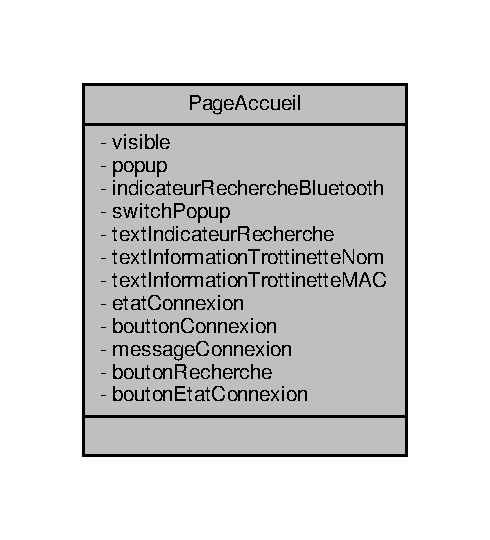
\includegraphics[width=235pt]{class_page_accueil__coll__graph}
\end{center}
\end{figure}
\subsubsection*{Attributs privés}
\begin{DoxyCompactItemize}
\item 
var \hyperlink{class_page_accueil_ae03956f235445b0802fbf9734b5c0388}{visible}
\item 
Popup \hyperlink{class_page_accueil_aba6d2877963eef2814a6fb7e994075de}{popup}
\item 
Busy\+Indicator \hyperlink{class_page_accueil_a52eb00d78f1e124f7157b76a0a971a46}{indicateur\+Recherche\+Bluetooth}
\item 
Switch \hyperlink{class_page_accueil_ae90456d8a42418d4657ddc563396b9da}{switch\+Popup}
\item 
Label \hyperlink{class_page_accueil_a808229add302b2754652774b07c90f75}{text\+Indicateur\+Recherche}
\item 
Label \hyperlink{class_page_accueil_acf7a4bb8798fe118632bf214600b56af}{text\+Information\+Trottinette\+Nom}
\item 
Label \hyperlink{class_page_accueil_ab5eca979dc44c0a4dc0f167fd1f37864}{text\+Information\+Trottinette\+M\+AC}
\item 
Label \hyperlink{class_page_accueil_a482152aaa6e321fab3b08c430b476f8f}{etat\+Connexion}
\item 
Button \hyperlink{class_page_accueil_a492c15a155aca7aae1fdab5bdbebedf2}{boutton\+Connexion}
\item 
Message\+Dialog \hyperlink{class_page_accueil_a094ce2a64386624d9443553a6524ca28}{message\+Connexion}
\item 
Button \hyperlink{class_page_accueil_a7efda9a58fdc87fad2bd6cdb60ec37d5}{bouton\+Recherche}
\item 
Button \hyperlink{class_page_accueil_ab974023098658affd679fc4c37ba945c}{bouton\+Etat\+Connexion}
\end{DoxyCompactItemize}


\subsubsection{Description détaillée}
\begin{DoxyAuthor}{Auteur}
Somphon Sy
\end{DoxyAuthor}
\begin{DoxyVersion}{Version}
1.\+1 
\end{DoxyVersion}


\subsubsection{Documentation des données membres}
\mbox{\Hypertarget{class_page_accueil_ab974023098658affd679fc4c37ba945c}\label{class_page_accueil_ab974023098658affd679fc4c37ba945c}} 
\index{Page\+Accueil@{Page\+Accueil}!bouton\+Etat\+Connexion@{bouton\+Etat\+Connexion}}
\index{bouton\+Etat\+Connexion@{bouton\+Etat\+Connexion}!Page\+Accueil@{Page\+Accueil}}
\paragraph{\texorpdfstring{bouton\+Etat\+Connexion}{boutonEtatConnexion}}
{\footnotesize\ttfamily Button Page\+Accueil\+::bouton\+Etat\+Connexion\hspace{0.3cm}{\ttfamily [private]}}

\mbox{\Hypertarget{class_page_accueil_a7efda9a58fdc87fad2bd6cdb60ec37d5}\label{class_page_accueil_a7efda9a58fdc87fad2bd6cdb60ec37d5}} 
\index{Page\+Accueil@{Page\+Accueil}!bouton\+Recherche@{bouton\+Recherche}}
\index{bouton\+Recherche@{bouton\+Recherche}!Page\+Accueil@{Page\+Accueil}}
\paragraph{\texorpdfstring{bouton\+Recherche}{boutonRecherche}}
{\footnotesize\ttfamily Button Page\+Accueil\+::bouton\+Recherche\hspace{0.3cm}{\ttfamily [private]}}

\mbox{\Hypertarget{class_page_accueil_a492c15a155aca7aae1fdab5bdbebedf2}\label{class_page_accueil_a492c15a155aca7aae1fdab5bdbebedf2}} 
\index{Page\+Accueil@{Page\+Accueil}!boutton\+Connexion@{boutton\+Connexion}}
\index{boutton\+Connexion@{boutton\+Connexion}!Page\+Accueil@{Page\+Accueil}}
\paragraph{\texorpdfstring{boutton\+Connexion}{bouttonConnexion}}
{\footnotesize\ttfamily Button Page\+Accueil\+::boutton\+Connexion\hspace{0.3cm}{\ttfamily [private]}}

\mbox{\Hypertarget{class_page_accueil_a482152aaa6e321fab3b08c430b476f8f}\label{class_page_accueil_a482152aaa6e321fab3b08c430b476f8f}} 
\index{Page\+Accueil@{Page\+Accueil}!etat\+Connexion@{etat\+Connexion}}
\index{etat\+Connexion@{etat\+Connexion}!Page\+Accueil@{Page\+Accueil}}
\paragraph{\texorpdfstring{etat\+Connexion}{etatConnexion}}
{\footnotesize\ttfamily Label Page\+Accueil\+::etat\+Connexion\hspace{0.3cm}{\ttfamily [private]}}

\mbox{\Hypertarget{class_page_accueil_a52eb00d78f1e124f7157b76a0a971a46}\label{class_page_accueil_a52eb00d78f1e124f7157b76a0a971a46}} 
\index{Page\+Accueil@{Page\+Accueil}!indicateur\+Recherche\+Bluetooth@{indicateur\+Recherche\+Bluetooth}}
\index{indicateur\+Recherche\+Bluetooth@{indicateur\+Recherche\+Bluetooth}!Page\+Accueil@{Page\+Accueil}}
\paragraph{\texorpdfstring{indicateur\+Recherche\+Bluetooth}{indicateurRechercheBluetooth}}
{\footnotesize\ttfamily Busy\+Indicator Page\+Accueil\+::indicateur\+Recherche\+Bluetooth\hspace{0.3cm}{\ttfamily [private]}}

\mbox{\Hypertarget{class_page_accueil_a094ce2a64386624d9443553a6524ca28}\label{class_page_accueil_a094ce2a64386624d9443553a6524ca28}} 
\index{Page\+Accueil@{Page\+Accueil}!message\+Connexion@{message\+Connexion}}
\index{message\+Connexion@{message\+Connexion}!Page\+Accueil@{Page\+Accueil}}
\paragraph{\texorpdfstring{message\+Connexion}{messageConnexion}}
{\footnotesize\ttfamily Message\+Dialog Page\+Accueil\+::message\+Connexion\hspace{0.3cm}{\ttfamily [private]}}

\mbox{\Hypertarget{class_page_accueil_aba6d2877963eef2814a6fb7e994075de}\label{class_page_accueil_aba6d2877963eef2814a6fb7e994075de}} 
\index{Page\+Accueil@{Page\+Accueil}!popup@{popup}}
\index{popup@{popup}!Page\+Accueil@{Page\+Accueil}}
\paragraph{\texorpdfstring{popup}{popup}}
{\footnotesize\ttfamily Popup Page\+Accueil\+::popup\hspace{0.3cm}{\ttfamily [private]}}

\mbox{\Hypertarget{class_page_accueil_ae90456d8a42418d4657ddc563396b9da}\label{class_page_accueil_ae90456d8a42418d4657ddc563396b9da}} 
\index{Page\+Accueil@{Page\+Accueil}!switch\+Popup@{switch\+Popup}}
\index{switch\+Popup@{switch\+Popup}!Page\+Accueil@{Page\+Accueil}}
\paragraph{\texorpdfstring{switch\+Popup}{switchPopup}}
{\footnotesize\ttfamily Switch Page\+Accueil\+::switch\+Popup\hspace{0.3cm}{\ttfamily [private]}}

\mbox{\Hypertarget{class_page_accueil_a808229add302b2754652774b07c90f75}\label{class_page_accueil_a808229add302b2754652774b07c90f75}} 
\index{Page\+Accueil@{Page\+Accueil}!text\+Indicateur\+Recherche@{text\+Indicateur\+Recherche}}
\index{text\+Indicateur\+Recherche@{text\+Indicateur\+Recherche}!Page\+Accueil@{Page\+Accueil}}
\paragraph{\texorpdfstring{text\+Indicateur\+Recherche}{textIndicateurRecherche}}
{\footnotesize\ttfamily Label Page\+Accueil\+::text\+Indicateur\+Recherche\hspace{0.3cm}{\ttfamily [private]}}

\mbox{\Hypertarget{class_page_accueil_ab5eca979dc44c0a4dc0f167fd1f37864}\label{class_page_accueil_ab5eca979dc44c0a4dc0f167fd1f37864}} 
\index{Page\+Accueil@{Page\+Accueil}!text\+Information\+Trottinette\+M\+AC@{text\+Information\+Trottinette\+M\+AC}}
\index{text\+Information\+Trottinette\+M\+AC@{text\+Information\+Trottinette\+M\+AC}!Page\+Accueil@{Page\+Accueil}}
\paragraph{\texorpdfstring{text\+Information\+Trottinette\+M\+AC}{textInformationTrottinetteMAC}}
{\footnotesize\ttfamily Label Page\+Accueil\+::text\+Information\+Trottinette\+M\+AC\hspace{0.3cm}{\ttfamily [private]}}

\mbox{\Hypertarget{class_page_accueil_acf7a4bb8798fe118632bf214600b56af}\label{class_page_accueil_acf7a4bb8798fe118632bf214600b56af}} 
\index{Page\+Accueil@{Page\+Accueil}!text\+Information\+Trottinette\+Nom@{text\+Information\+Trottinette\+Nom}}
\index{text\+Information\+Trottinette\+Nom@{text\+Information\+Trottinette\+Nom}!Page\+Accueil@{Page\+Accueil}}
\paragraph{\texorpdfstring{text\+Information\+Trottinette\+Nom}{textInformationTrottinetteNom}}
{\footnotesize\ttfamily Label Page\+Accueil\+::text\+Information\+Trottinette\+Nom\hspace{0.3cm}{\ttfamily [private]}}

\mbox{\Hypertarget{class_page_accueil_ae03956f235445b0802fbf9734b5c0388}\label{class_page_accueil_ae03956f235445b0802fbf9734b5c0388}} 
\index{Page\+Accueil@{Page\+Accueil}!visible@{visible}}
\index{visible@{visible}!Page\+Accueil@{Page\+Accueil}}
\paragraph{\texorpdfstring{visible}{visible}}
{\footnotesize\ttfamily var Page\+Accueil\+::visible\hspace{0.3cm}{\ttfamily [private]}}



La documentation de cette classe a été générée à partir du fichier suivant \+:\begin{DoxyCompactItemize}
\item 
\hyperlink{_page_accueil_8qml}{Page\+Accueil.\+qml}\end{DoxyCompactItemize}

\hypertarget{class_page_carte}{}\subsection{Référence de la classe Page\+Carte}
\label{class_page_carte}\index{Page\+Carte@{Page\+Carte}}


La page de navigation (Carte et/ou Télémétrie)  




Graphe de collaboration de Page\+Carte\+:\nopagebreak
\begin{figure}[H]
\begin{center}
\leavevmode
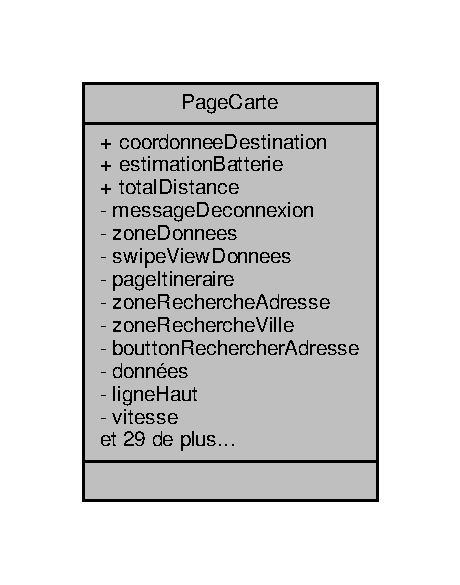
\includegraphics[width=221pt]{class_page_carte__coll__graph}
\end{center}
\end{figure}
\subsubsection*{Propriétés}
\begin{DoxyCompactItemize}
\item 
variant \hyperlink{class_page_carte_ae010768ed12ad9729c2c9b62469212e6}{coordonnee\+Destination}
\item 
int \hyperlink{class_page_carte_a6881b3f806dbfe3c5d187458e57d25b9}{estimation\+Batterie}
\item 
string \hyperlink{class_page_carte_ac82c3aebfbfa75f8da8cd1add5b18339}{total\+Distance}
\end{DoxyCompactItemize}
\subsubsection*{Attributs privés}
\begin{DoxyCompactItemize}
\item 
Message\+Dialog \hyperlink{class_page_carte_a568c9ee2a559b645ee3914ea36d19156}{message\+Deconnexion}
\item 
Rectangle \hyperlink{class_page_carte_a7e177e62466f97f757bcde0b45d0f461}{zone\+Donnees}
\item 
Swipe\+View \hyperlink{class_page_carte_ae741a4d5edd58f96788fa0e108e69cd4}{swipe\+View\+Donnees}
\item 
Page \hyperlink{class_page_carte_afad501d1f18a3665dfc6756f24a634e2}{page\+Itineraire}
\item 
Text\+Field \hyperlink{class_page_carte_a01dbcc8cc00107fb4ef3bc617540ee08}{zone\+Recherche\+Adresse}
\item 
Text\+Field \hyperlink{class_page_carte_ace51a569f45a195e0dc2e3bcc5f4f455}{zone\+Recherche\+Ville}
\item 
Button \hyperlink{class_page_carte_a11a85cfcce643c839e4b5d0be82841dc}{boutton\+Rechercher\+Adresse}
\item 
Page \hyperlink{class_page_carte_a056a17cfc7555356e2c1be58ad696a8c}{données}
\item 
Row\+Layout \hyperlink{class_page_carte_a4bbd7bd1bcbf52d6b1a02e6b7f1f787c}{ligne\+Haut}
\item 
Label \hyperlink{class_page_carte_ac6738468ea4cd409417060a8818603fb}{vitesse}
\item 
Text \hyperlink{class_page_carte_ab1e75b382dac00215c0e3ab4f33d3d66}{indicateur\+Vitesse}
\item 
Column \hyperlink{class_page_carte_a92dd7965b19b538f5a4b91fd1da11829}{colonne\+Batterie}
\item 
Label \hyperlink{class_page_carte_a91f6a01493a0831c19556991a757cf72}{batterie}
\item 
Text \hyperlink{class_page_carte_aa0bc82b7aa8ff7488ab3689b4a5c743d}{indicateur\+Batterie}
\item 
Label \hyperlink{class_page_carte_aaefd6baa99ea0d8b545cc85bee0cff49}{inclinaison}
\item 
Text \hyperlink{class_page_carte_a836b08dfd760281849e6d512e270e64e}{indicateur\+Inclinaison}
\item 
Row\+Layout \hyperlink{class_page_carte_a1d1f4e766052166c348f1b5fae56a474}{ligne\+Bas}
\item 
Label \hyperlink{class_page_carte_a034ebe3a106110dc22f5ee8bae18f87b}{distance\+Parcourue}
\item 
Text \hyperlink{class_page_carte_a9741edd97f3bbffe384094090736900c}{indicateur\+Distance\+Parcourue}
\item 
Label \hyperlink{class_page_carte_a277e3b7d3dcba3a675e853122a45109e}{duree\+Utilisation}
\item 
Text \hyperlink{class_page_carte_aec12ab9dfdb0165276f6f41fcaa0525b}{indicateurduree\+Utilisation}
\item 
Tab\+Bar \hyperlink{class_page_carte_acca3b766f8874214b8300344c094dbbe}{onglets\+Donnees}
\item 
Rectangle \hyperlink{class_page_carte_a71510c3afaf8914bd7800d7f41cf4572}{affichage\+Carte}
\item 
Plugin \hyperlink{class_page_carte_a4e63a00c2287b930a49c821781997814}{map\+Plugin}
\item 
Map \hyperlink{class_page_carte_aacb6261b77a9d463379aa17305938cce}{map}
\item 
Map\+Quick\+Item \hyperlink{class_page_carte_a40b7fe9e6f8250856b923b042c97a5a5}{indicateur\+Position}
\item 
Map\+Quick\+Item \hyperlink{class_page_carte_ac957f423cdb504fe0e023cbc94322dd5}{marqueur\+Arrivee}
\item 
Image \hyperlink{class_page_carte_ae599f81f24a82946f75f68e85cafccbc}{etat\+Connexion\+Bluetooth\+Carte}
\item 
Image \hyperlink{class_page_carte_a5a73e49abed67e634aca9eaff4dff7f7}{etat\+Batterie\+Trottinette\+Carte}
\item 
Image \hyperlink{class_page_carte_ace08a458300ff3f9de709d257d35d175}{indicateur\+Risque\+De\+Chute}
\item 
Text \hyperlink{class_page_carte_aea49b9971ff80ccdc4eb9aba4b0fcc55}{distance\+Totale}
\item 
Text \hyperlink{class_page_carte_aaaaa7273751a2db869c16c7cd02e2b9a}{estimation}
\item 
Button \hyperlink{class_page_carte_a9d6fd98e7c648783f9865b2839665b10}{zoom\+Plus}
\item 
Button \hyperlink{class_page_carte_a4644424e3d5e139af73dec85c500d74d}{zoom\+Moins}
\item 
Button \hyperlink{class_page_carte_afb27dfd099ed625fa8d4fab997ff421e}{boutton\+Centre}
\item 
Position\+Source \hyperlink{class_page_carte_a601b30458f6e0a27f670522a69aebc89}{src}
\item 
Route\+Model \hyperlink{class_page_carte_a4bef895ff3ef4f2c89ba1f202d8500a9}{itineraire}
\item 
Geocode\+Model \hyperlink{class_page_carte_a67834fc06727ceb87a4ac2dc40025a44}{adresse\+Recherche}
\item 
Geocode\+Model \hyperlink{class_page_carte_a66dc1e3837176828499ec7f388278b61}{adresse\+Localisation}
\end{DoxyCompactItemize}


\subsubsection{Description détaillée}
\begin{DoxyAuthor}{Auteur}
Somphon Sy
\end{DoxyAuthor}
\begin{DoxyVersion}{Version}
1.\+1 
\end{DoxyVersion}


\subsubsection{Documentation des données membres}
\mbox{\Hypertarget{class_page_carte_a66dc1e3837176828499ec7f388278b61}\label{class_page_carte_a66dc1e3837176828499ec7f388278b61}} 
\index{Page\+Carte@{Page\+Carte}!adresse\+Localisation@{adresse\+Localisation}}
\index{adresse\+Localisation@{adresse\+Localisation}!Page\+Carte@{Page\+Carte}}
\paragraph{\texorpdfstring{adresse\+Localisation}{adresseLocalisation}}
{\footnotesize\ttfamily Geocode\+Model Page\+Carte\+::adresse\+Localisation\hspace{0.3cm}{\ttfamily [private]}}

\mbox{\Hypertarget{class_page_carte_a67834fc06727ceb87a4ac2dc40025a44}\label{class_page_carte_a67834fc06727ceb87a4ac2dc40025a44}} 
\index{Page\+Carte@{Page\+Carte}!adresse\+Recherche@{adresse\+Recherche}}
\index{adresse\+Recherche@{adresse\+Recherche}!Page\+Carte@{Page\+Carte}}
\paragraph{\texorpdfstring{adresse\+Recherche}{adresseRecherche}}
{\footnotesize\ttfamily Geocode\+Model Page\+Carte\+::adresse\+Recherche\hspace{0.3cm}{\ttfamily [private]}}

\mbox{\Hypertarget{class_page_carte_a71510c3afaf8914bd7800d7f41cf4572}\label{class_page_carte_a71510c3afaf8914bd7800d7f41cf4572}} 
\index{Page\+Carte@{Page\+Carte}!affichage\+Carte@{affichage\+Carte}}
\index{affichage\+Carte@{affichage\+Carte}!Page\+Carte@{Page\+Carte}}
\paragraph{\texorpdfstring{affichage\+Carte}{affichageCarte}}
{\footnotesize\ttfamily Rectangle Page\+Carte\+::affichage\+Carte\hspace{0.3cm}{\ttfamily [private]}}

\mbox{\Hypertarget{class_page_carte_a91f6a01493a0831c19556991a757cf72}\label{class_page_carte_a91f6a01493a0831c19556991a757cf72}} 
\index{Page\+Carte@{Page\+Carte}!batterie@{batterie}}
\index{batterie@{batterie}!Page\+Carte@{Page\+Carte}}
\paragraph{\texorpdfstring{batterie}{batterie}}
{\footnotesize\ttfamily Label Page\+Carte\+::batterie\hspace{0.3cm}{\ttfamily [private]}}

\mbox{\Hypertarget{class_page_carte_afb27dfd099ed625fa8d4fab997ff421e}\label{class_page_carte_afb27dfd099ed625fa8d4fab997ff421e}} 
\index{Page\+Carte@{Page\+Carte}!boutton\+Centre@{boutton\+Centre}}
\index{boutton\+Centre@{boutton\+Centre}!Page\+Carte@{Page\+Carte}}
\paragraph{\texorpdfstring{boutton\+Centre}{bouttonCentre}}
{\footnotesize\ttfamily Button Page\+Carte\+::boutton\+Centre\hspace{0.3cm}{\ttfamily [private]}}

\mbox{\Hypertarget{class_page_carte_a11a85cfcce643c839e4b5d0be82841dc}\label{class_page_carte_a11a85cfcce643c839e4b5d0be82841dc}} 
\index{Page\+Carte@{Page\+Carte}!boutton\+Rechercher\+Adresse@{boutton\+Rechercher\+Adresse}}
\index{boutton\+Rechercher\+Adresse@{boutton\+Rechercher\+Adresse}!Page\+Carte@{Page\+Carte}}
\paragraph{\texorpdfstring{boutton\+Rechercher\+Adresse}{bouttonRechercherAdresse}}
{\footnotesize\ttfamily Button Page\+Carte\+::boutton\+Rechercher\+Adresse\hspace{0.3cm}{\ttfamily [private]}}

\mbox{\Hypertarget{class_page_carte_a92dd7965b19b538f5a4b91fd1da11829}\label{class_page_carte_a92dd7965b19b538f5a4b91fd1da11829}} 
\index{Page\+Carte@{Page\+Carte}!colonne\+Batterie@{colonne\+Batterie}}
\index{colonne\+Batterie@{colonne\+Batterie}!Page\+Carte@{Page\+Carte}}
\paragraph{\texorpdfstring{colonne\+Batterie}{colonneBatterie}}
{\footnotesize\ttfamily Column Page\+Carte\+::colonne\+Batterie\hspace{0.3cm}{\ttfamily [private]}}

\mbox{\Hypertarget{class_page_carte_a034ebe3a106110dc22f5ee8bae18f87b}\label{class_page_carte_a034ebe3a106110dc22f5ee8bae18f87b}} 
\index{Page\+Carte@{Page\+Carte}!distance\+Parcourue@{distance\+Parcourue}}
\index{distance\+Parcourue@{distance\+Parcourue}!Page\+Carte@{Page\+Carte}}
\paragraph{\texorpdfstring{distance\+Parcourue}{distanceParcourue}}
{\footnotesize\ttfamily Label Page\+Carte\+::distance\+Parcourue\hspace{0.3cm}{\ttfamily [private]}}

\mbox{\Hypertarget{class_page_carte_aea49b9971ff80ccdc4eb9aba4b0fcc55}\label{class_page_carte_aea49b9971ff80ccdc4eb9aba4b0fcc55}} 
\index{Page\+Carte@{Page\+Carte}!distance\+Totale@{distance\+Totale}}
\index{distance\+Totale@{distance\+Totale}!Page\+Carte@{Page\+Carte}}
\paragraph{\texorpdfstring{distance\+Totale}{distanceTotale}}
{\footnotesize\ttfamily Text Page\+Carte\+::distance\+Totale\hspace{0.3cm}{\ttfamily [private]}}

\mbox{\Hypertarget{class_page_carte_a056a17cfc7555356e2c1be58ad696a8c}\label{class_page_carte_a056a17cfc7555356e2c1be58ad696a8c}} 
\index{Page\+Carte@{Page\+Carte}!données@{données}}
\index{données@{données}!Page\+Carte@{Page\+Carte}}
\paragraph{\texorpdfstring{données}{données}}
{\footnotesize\ttfamily Page Page\+Carte\+::données\hspace{0.3cm}{\ttfamily [private]}}

\mbox{\Hypertarget{class_page_carte_a277e3b7d3dcba3a675e853122a45109e}\label{class_page_carte_a277e3b7d3dcba3a675e853122a45109e}} 
\index{Page\+Carte@{Page\+Carte}!duree\+Utilisation@{duree\+Utilisation}}
\index{duree\+Utilisation@{duree\+Utilisation}!Page\+Carte@{Page\+Carte}}
\paragraph{\texorpdfstring{duree\+Utilisation}{dureeUtilisation}}
{\footnotesize\ttfamily Label Page\+Carte\+::duree\+Utilisation\hspace{0.3cm}{\ttfamily [private]}}

\mbox{\Hypertarget{class_page_carte_aaaaa7273751a2db869c16c7cd02e2b9a}\label{class_page_carte_aaaaa7273751a2db869c16c7cd02e2b9a}} 
\index{Page\+Carte@{Page\+Carte}!estimation@{estimation}}
\index{estimation@{estimation}!Page\+Carte@{Page\+Carte}}
\paragraph{\texorpdfstring{estimation}{estimation}}
{\footnotesize\ttfamily Text Page\+Carte\+::estimation\hspace{0.3cm}{\ttfamily [private]}}

\mbox{\Hypertarget{class_page_carte_a5a73e49abed67e634aca9eaff4dff7f7}\label{class_page_carte_a5a73e49abed67e634aca9eaff4dff7f7}} 
\index{Page\+Carte@{Page\+Carte}!etat\+Batterie\+Trottinette\+Carte@{etat\+Batterie\+Trottinette\+Carte}}
\index{etat\+Batterie\+Trottinette\+Carte@{etat\+Batterie\+Trottinette\+Carte}!Page\+Carte@{Page\+Carte}}
\paragraph{\texorpdfstring{etat\+Batterie\+Trottinette\+Carte}{etatBatterieTrottinetteCarte}}
{\footnotesize\ttfamily Image Page\+Carte\+::etat\+Batterie\+Trottinette\+Carte\hspace{0.3cm}{\ttfamily [private]}}

\mbox{\Hypertarget{class_page_carte_ae599f81f24a82946f75f68e85cafccbc}\label{class_page_carte_ae599f81f24a82946f75f68e85cafccbc}} 
\index{Page\+Carte@{Page\+Carte}!etat\+Connexion\+Bluetooth\+Carte@{etat\+Connexion\+Bluetooth\+Carte}}
\index{etat\+Connexion\+Bluetooth\+Carte@{etat\+Connexion\+Bluetooth\+Carte}!Page\+Carte@{Page\+Carte}}
\paragraph{\texorpdfstring{etat\+Connexion\+Bluetooth\+Carte}{etatConnexionBluetoothCarte}}
{\footnotesize\ttfamily Image Page\+Carte\+::etat\+Connexion\+Bluetooth\+Carte\hspace{0.3cm}{\ttfamily [private]}}

\mbox{\Hypertarget{class_page_carte_aaefd6baa99ea0d8b545cc85bee0cff49}\label{class_page_carte_aaefd6baa99ea0d8b545cc85bee0cff49}} 
\index{Page\+Carte@{Page\+Carte}!inclinaison@{inclinaison}}
\index{inclinaison@{inclinaison}!Page\+Carte@{Page\+Carte}}
\paragraph{\texorpdfstring{inclinaison}{inclinaison}}
{\footnotesize\ttfamily Label Page\+Carte\+::inclinaison\hspace{0.3cm}{\ttfamily [private]}}

\mbox{\Hypertarget{class_page_carte_aa0bc82b7aa8ff7488ab3689b4a5c743d}\label{class_page_carte_aa0bc82b7aa8ff7488ab3689b4a5c743d}} 
\index{Page\+Carte@{Page\+Carte}!indicateur\+Batterie@{indicateur\+Batterie}}
\index{indicateur\+Batterie@{indicateur\+Batterie}!Page\+Carte@{Page\+Carte}}
\paragraph{\texorpdfstring{indicateur\+Batterie}{indicateurBatterie}}
{\footnotesize\ttfamily Text Page\+Carte\+::indicateur\+Batterie\hspace{0.3cm}{\ttfamily [private]}}

\mbox{\Hypertarget{class_page_carte_a9741edd97f3bbffe384094090736900c}\label{class_page_carte_a9741edd97f3bbffe384094090736900c}} 
\index{Page\+Carte@{Page\+Carte}!indicateur\+Distance\+Parcourue@{indicateur\+Distance\+Parcourue}}
\index{indicateur\+Distance\+Parcourue@{indicateur\+Distance\+Parcourue}!Page\+Carte@{Page\+Carte}}
\paragraph{\texorpdfstring{indicateur\+Distance\+Parcourue}{indicateurDistanceParcourue}}
{\footnotesize\ttfamily Text Page\+Carte\+::indicateur\+Distance\+Parcourue\hspace{0.3cm}{\ttfamily [private]}}

\mbox{\Hypertarget{class_page_carte_aec12ab9dfdb0165276f6f41fcaa0525b}\label{class_page_carte_aec12ab9dfdb0165276f6f41fcaa0525b}} 
\index{Page\+Carte@{Page\+Carte}!indicateurduree\+Utilisation@{indicateurduree\+Utilisation}}
\index{indicateurduree\+Utilisation@{indicateurduree\+Utilisation}!Page\+Carte@{Page\+Carte}}
\paragraph{\texorpdfstring{indicateurduree\+Utilisation}{indicateurdureeUtilisation}}
{\footnotesize\ttfamily Text Page\+Carte\+::indicateurduree\+Utilisation\hspace{0.3cm}{\ttfamily [private]}}

\mbox{\Hypertarget{class_page_carte_a836b08dfd760281849e6d512e270e64e}\label{class_page_carte_a836b08dfd760281849e6d512e270e64e}} 
\index{Page\+Carte@{Page\+Carte}!indicateur\+Inclinaison@{indicateur\+Inclinaison}}
\index{indicateur\+Inclinaison@{indicateur\+Inclinaison}!Page\+Carte@{Page\+Carte}}
\paragraph{\texorpdfstring{indicateur\+Inclinaison}{indicateurInclinaison}}
{\footnotesize\ttfamily Text Page\+Carte\+::indicateur\+Inclinaison\hspace{0.3cm}{\ttfamily [private]}}

\mbox{\Hypertarget{class_page_carte_a40b7fe9e6f8250856b923b042c97a5a5}\label{class_page_carte_a40b7fe9e6f8250856b923b042c97a5a5}} 
\index{Page\+Carte@{Page\+Carte}!indicateur\+Position@{indicateur\+Position}}
\index{indicateur\+Position@{indicateur\+Position}!Page\+Carte@{Page\+Carte}}
\paragraph{\texorpdfstring{indicateur\+Position}{indicateurPosition}}
{\footnotesize\ttfamily Map\+Quick\+Item Page\+Carte\+::indicateur\+Position\hspace{0.3cm}{\ttfamily [private]}}

\mbox{\Hypertarget{class_page_carte_ace08a458300ff3f9de709d257d35d175}\label{class_page_carte_ace08a458300ff3f9de709d257d35d175}} 
\index{Page\+Carte@{Page\+Carte}!indicateur\+Risque\+De\+Chute@{indicateur\+Risque\+De\+Chute}}
\index{indicateur\+Risque\+De\+Chute@{indicateur\+Risque\+De\+Chute}!Page\+Carte@{Page\+Carte}}
\paragraph{\texorpdfstring{indicateur\+Risque\+De\+Chute}{indicateurRisqueDeChute}}
{\footnotesize\ttfamily Image Page\+Carte\+::indicateur\+Risque\+De\+Chute\hspace{0.3cm}{\ttfamily [private]}}

\mbox{\Hypertarget{class_page_carte_ab1e75b382dac00215c0e3ab4f33d3d66}\label{class_page_carte_ab1e75b382dac00215c0e3ab4f33d3d66}} 
\index{Page\+Carte@{Page\+Carte}!indicateur\+Vitesse@{indicateur\+Vitesse}}
\index{indicateur\+Vitesse@{indicateur\+Vitesse}!Page\+Carte@{Page\+Carte}}
\paragraph{\texorpdfstring{indicateur\+Vitesse}{indicateurVitesse}}
{\footnotesize\ttfamily Text Page\+Carte\+::indicateur\+Vitesse\hspace{0.3cm}{\ttfamily [private]}}

\mbox{\Hypertarget{class_page_carte_a4bef895ff3ef4f2c89ba1f202d8500a9}\label{class_page_carte_a4bef895ff3ef4f2c89ba1f202d8500a9}} 
\index{Page\+Carte@{Page\+Carte}!itineraire@{itineraire}}
\index{itineraire@{itineraire}!Page\+Carte@{Page\+Carte}}
\paragraph{\texorpdfstring{itineraire}{itineraire}}
{\footnotesize\ttfamily Route\+Model Page\+Carte\+::itineraire\hspace{0.3cm}{\ttfamily [private]}}

\mbox{\Hypertarget{class_page_carte_a1d1f4e766052166c348f1b5fae56a474}\label{class_page_carte_a1d1f4e766052166c348f1b5fae56a474}} 
\index{Page\+Carte@{Page\+Carte}!ligne\+Bas@{ligne\+Bas}}
\index{ligne\+Bas@{ligne\+Bas}!Page\+Carte@{Page\+Carte}}
\paragraph{\texorpdfstring{ligne\+Bas}{ligneBas}}
{\footnotesize\ttfamily Row\+Layout Page\+Carte\+::ligne\+Bas\hspace{0.3cm}{\ttfamily [private]}}

\mbox{\Hypertarget{class_page_carte_a4bbd7bd1bcbf52d6b1a02e6b7f1f787c}\label{class_page_carte_a4bbd7bd1bcbf52d6b1a02e6b7f1f787c}} 
\index{Page\+Carte@{Page\+Carte}!ligne\+Haut@{ligne\+Haut}}
\index{ligne\+Haut@{ligne\+Haut}!Page\+Carte@{Page\+Carte}}
\paragraph{\texorpdfstring{ligne\+Haut}{ligneHaut}}
{\footnotesize\ttfamily Row\+Layout Page\+Carte\+::ligne\+Haut\hspace{0.3cm}{\ttfamily [private]}}

\mbox{\Hypertarget{class_page_carte_aacb6261b77a9d463379aa17305938cce}\label{class_page_carte_aacb6261b77a9d463379aa17305938cce}} 
\index{Page\+Carte@{Page\+Carte}!map@{map}}
\index{map@{map}!Page\+Carte@{Page\+Carte}}
\paragraph{\texorpdfstring{map}{map}}
{\footnotesize\ttfamily Map Page\+Carte\+::map\hspace{0.3cm}{\ttfamily [private]}}

\mbox{\Hypertarget{class_page_carte_a4e63a00c2287b930a49c821781997814}\label{class_page_carte_a4e63a00c2287b930a49c821781997814}} 
\index{Page\+Carte@{Page\+Carte}!map\+Plugin@{map\+Plugin}}
\index{map\+Plugin@{map\+Plugin}!Page\+Carte@{Page\+Carte}}
\paragraph{\texorpdfstring{map\+Plugin}{mapPlugin}}
{\footnotesize\ttfamily Plugin Page\+Carte\+::map\+Plugin\hspace{0.3cm}{\ttfamily [private]}}

\mbox{\Hypertarget{class_page_carte_ac957f423cdb504fe0e023cbc94322dd5}\label{class_page_carte_ac957f423cdb504fe0e023cbc94322dd5}} 
\index{Page\+Carte@{Page\+Carte}!marqueur\+Arrivee@{marqueur\+Arrivee}}
\index{marqueur\+Arrivee@{marqueur\+Arrivee}!Page\+Carte@{Page\+Carte}}
\paragraph{\texorpdfstring{marqueur\+Arrivee}{marqueurArrivee}}
{\footnotesize\ttfamily Map\+Quick\+Item Page\+Carte\+::marqueur\+Arrivee\hspace{0.3cm}{\ttfamily [private]}}

\mbox{\Hypertarget{class_page_carte_a568c9ee2a559b645ee3914ea36d19156}\label{class_page_carte_a568c9ee2a559b645ee3914ea36d19156}} 
\index{Page\+Carte@{Page\+Carte}!message\+Deconnexion@{message\+Deconnexion}}
\index{message\+Deconnexion@{message\+Deconnexion}!Page\+Carte@{Page\+Carte}}
\paragraph{\texorpdfstring{message\+Deconnexion}{messageDeconnexion}}
{\footnotesize\ttfamily Message\+Dialog Page\+Carte\+::message\+Deconnexion\hspace{0.3cm}{\ttfamily [private]}}

\mbox{\Hypertarget{class_page_carte_acca3b766f8874214b8300344c094dbbe}\label{class_page_carte_acca3b766f8874214b8300344c094dbbe}} 
\index{Page\+Carte@{Page\+Carte}!onglets\+Donnees@{onglets\+Donnees}}
\index{onglets\+Donnees@{onglets\+Donnees}!Page\+Carte@{Page\+Carte}}
\paragraph{\texorpdfstring{onglets\+Donnees}{ongletsDonnees}}
{\footnotesize\ttfamily Tab\+Bar Page\+Carte\+::onglets\+Donnees\hspace{0.3cm}{\ttfamily [private]}}

\mbox{\Hypertarget{class_page_carte_afad501d1f18a3665dfc6756f24a634e2}\label{class_page_carte_afad501d1f18a3665dfc6756f24a634e2}} 
\index{Page\+Carte@{Page\+Carte}!page\+Itineraire@{page\+Itineraire}}
\index{page\+Itineraire@{page\+Itineraire}!Page\+Carte@{Page\+Carte}}
\paragraph{\texorpdfstring{page\+Itineraire}{pageItineraire}}
{\footnotesize\ttfamily Page Page\+Carte\+::page\+Itineraire\hspace{0.3cm}{\ttfamily [private]}}

\mbox{\Hypertarget{class_page_carte_a601b30458f6e0a27f670522a69aebc89}\label{class_page_carte_a601b30458f6e0a27f670522a69aebc89}} 
\index{Page\+Carte@{Page\+Carte}!src@{src}}
\index{src@{src}!Page\+Carte@{Page\+Carte}}
\paragraph{\texorpdfstring{src}{src}}
{\footnotesize\ttfamily Position\+Source Page\+Carte\+::src\hspace{0.3cm}{\ttfamily [private]}}

\mbox{\Hypertarget{class_page_carte_ae741a4d5edd58f96788fa0e108e69cd4}\label{class_page_carte_ae741a4d5edd58f96788fa0e108e69cd4}} 
\index{Page\+Carte@{Page\+Carte}!swipe\+View\+Donnees@{swipe\+View\+Donnees}}
\index{swipe\+View\+Donnees@{swipe\+View\+Donnees}!Page\+Carte@{Page\+Carte}}
\paragraph{\texorpdfstring{swipe\+View\+Donnees}{swipeViewDonnees}}
{\footnotesize\ttfamily Swipe\+View Page\+Carte\+::swipe\+View\+Donnees\hspace{0.3cm}{\ttfamily [private]}}

\mbox{\Hypertarget{class_page_carte_ac6738468ea4cd409417060a8818603fb}\label{class_page_carte_ac6738468ea4cd409417060a8818603fb}} 
\index{Page\+Carte@{Page\+Carte}!vitesse@{vitesse}}
\index{vitesse@{vitesse}!Page\+Carte@{Page\+Carte}}
\paragraph{\texorpdfstring{vitesse}{vitesse}}
{\footnotesize\ttfamily Label Page\+Carte\+::vitesse\hspace{0.3cm}{\ttfamily [private]}}

\mbox{\Hypertarget{class_page_carte_a7e177e62466f97f757bcde0b45d0f461}\label{class_page_carte_a7e177e62466f97f757bcde0b45d0f461}} 
\index{Page\+Carte@{Page\+Carte}!zone\+Donnees@{zone\+Donnees}}
\index{zone\+Donnees@{zone\+Donnees}!Page\+Carte@{Page\+Carte}}
\paragraph{\texorpdfstring{zone\+Donnees}{zoneDonnees}}
{\footnotesize\ttfamily Rectangle Page\+Carte\+::zone\+Donnees\hspace{0.3cm}{\ttfamily [private]}}

\mbox{\Hypertarget{class_page_carte_a01dbcc8cc00107fb4ef3bc617540ee08}\label{class_page_carte_a01dbcc8cc00107fb4ef3bc617540ee08}} 
\index{Page\+Carte@{Page\+Carte}!zone\+Recherche\+Adresse@{zone\+Recherche\+Adresse}}
\index{zone\+Recherche\+Adresse@{zone\+Recherche\+Adresse}!Page\+Carte@{Page\+Carte}}
\paragraph{\texorpdfstring{zone\+Recherche\+Adresse}{zoneRechercheAdresse}}
{\footnotesize\ttfamily Text\+Field Page\+Carte\+::zone\+Recherche\+Adresse\hspace{0.3cm}{\ttfamily [private]}}

\mbox{\Hypertarget{class_page_carte_ace51a569f45a195e0dc2e3bcc5f4f455}\label{class_page_carte_ace51a569f45a195e0dc2e3bcc5f4f455}} 
\index{Page\+Carte@{Page\+Carte}!zone\+Recherche\+Ville@{zone\+Recherche\+Ville}}
\index{zone\+Recherche\+Ville@{zone\+Recherche\+Ville}!Page\+Carte@{Page\+Carte}}
\paragraph{\texorpdfstring{zone\+Recherche\+Ville}{zoneRechercheVille}}
{\footnotesize\ttfamily Text\+Field Page\+Carte\+::zone\+Recherche\+Ville\hspace{0.3cm}{\ttfamily [private]}}

\mbox{\Hypertarget{class_page_carte_a4644424e3d5e139af73dec85c500d74d}\label{class_page_carte_a4644424e3d5e139af73dec85c500d74d}} 
\index{Page\+Carte@{Page\+Carte}!zoom\+Moins@{zoom\+Moins}}
\index{zoom\+Moins@{zoom\+Moins}!Page\+Carte@{Page\+Carte}}
\paragraph{\texorpdfstring{zoom\+Moins}{zoomMoins}}
{\footnotesize\ttfamily Button Page\+Carte\+::zoom\+Moins\hspace{0.3cm}{\ttfamily [private]}}

\mbox{\Hypertarget{class_page_carte_a9d6fd98e7c648783f9865b2839665b10}\label{class_page_carte_a9d6fd98e7c648783f9865b2839665b10}} 
\index{Page\+Carte@{Page\+Carte}!zoom\+Plus@{zoom\+Plus}}
\index{zoom\+Plus@{zoom\+Plus}!Page\+Carte@{Page\+Carte}}
\paragraph{\texorpdfstring{zoom\+Plus}{zoomPlus}}
{\footnotesize\ttfamily Button Page\+Carte\+::zoom\+Plus\hspace{0.3cm}{\ttfamily [private]}}



\subsubsection{Documentation des propriétés}
\mbox{\Hypertarget{class_page_carte_ae010768ed12ad9729c2c9b62469212e6}\label{class_page_carte_ae010768ed12ad9729c2c9b62469212e6}} 
\index{Page\+Carte@{Page\+Carte}!coordonnee\+Destination@{coordonnee\+Destination}}
\index{coordonnee\+Destination@{coordonnee\+Destination}!Page\+Carte@{Page\+Carte}}
\paragraph{\texorpdfstring{coordonnee\+Destination}{coordonneeDestination}}
{\footnotesize\ttfamily variant Page\+Carte\+::coordonnee\+Destination}

\mbox{\Hypertarget{class_page_carte_a6881b3f806dbfe3c5d187458e57d25b9}\label{class_page_carte_a6881b3f806dbfe3c5d187458e57d25b9}} 
\index{Page\+Carte@{Page\+Carte}!estimation\+Batterie@{estimation\+Batterie}}
\index{estimation\+Batterie@{estimation\+Batterie}!Page\+Carte@{Page\+Carte}}
\paragraph{\texorpdfstring{estimation\+Batterie}{estimationBatterie}}
{\footnotesize\ttfamily int Page\+Carte\+::estimation\+Batterie}

\mbox{\Hypertarget{class_page_carte_ac82c3aebfbfa75f8da8cd1add5b18339}\label{class_page_carte_ac82c3aebfbfa75f8da8cd1add5b18339}} 
\index{Page\+Carte@{Page\+Carte}!total\+Distance@{total\+Distance}}
\index{total\+Distance@{total\+Distance}!Page\+Carte@{Page\+Carte}}
\paragraph{\texorpdfstring{total\+Distance}{totalDistance}}
{\footnotesize\ttfamily string Page\+Carte\+::total\+Distance}



La documentation de cette classe a été générée à partir du fichier suivant \+:\begin{DoxyCompactItemize}
\item 
\hyperlink{_page_carte_8qml}{Page\+Carte.\+qml}\end{DoxyCompactItemize}

\hypertarget{class_peripherique_local}{}\subsection{Référence de la classe Peripherique\+Local}
\label{class_peripherique_local}\index{Peripherique\+Local@{Peripherique\+Local}}


Déclaration de la classe \hyperlink{class_peripherique_local}{Peripherique\+Local}.  




{\ttfamily \#include $<$peripheriquelocal.\+h$>$}



Graphe de collaboration de Peripherique\+Local\+:
\nopagebreak
\begin{figure}[H]
\begin{center}
\leavevmode
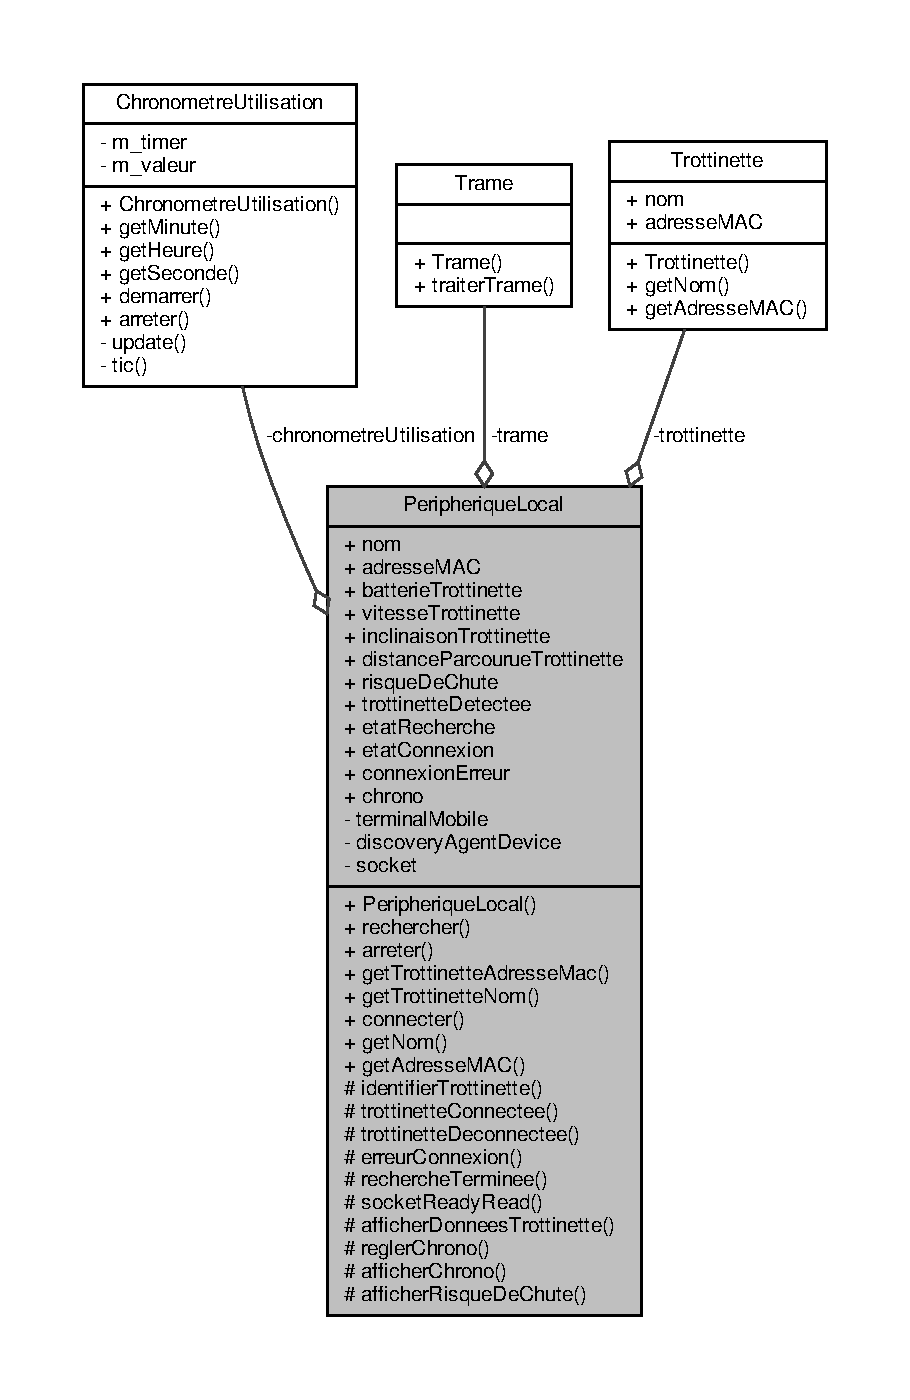
\includegraphics[width=350pt]{class_peripherique_local__coll__graph}
\end{center}
\end{figure}
\subsubsection*{Signaux}
\begin{DoxyCompactItemize}
\item 
void \hyperlink{class_peripherique_local_a7495daea266cb24dec35d85c651bd4c5}{connecte} ()
\begin{DoxyCompactList}\small\item\em Signal émis lorsque la trottinette est connectée au périphérique Local. \end{DoxyCompactList}\item 
void \hyperlink{class_peripherique_local_a2a8f0b072821f6d76db20b6f73b6acd0}{deconnecte} ()
\begin{DoxyCompactList}\small\item\em Signal émis lorsque la trottinette est déconnectée du périphérique Local. \end{DoxyCompactList}\item 
void \hyperlink{class_peripherique_local_a017f86e371bad418585d28b97557248a}{recherche} ()
\begin{DoxyCompactList}\small\item\em Signal émis lorsque le périphérique Local recherche la trottinette. \end{DoxyCompactList}\item 
void \hyperlink{class_peripherique_local_a41d9e18f2fd7e8e872db5fd3f21b11ff}{erreur} ()
\begin{DoxyCompactList}\small\item\em Signal émis lorsque qu\textquotesingle{}il y a une erreur de connexion entre la trottinette et le périphérique Local. \end{DoxyCompactList}\item 
void \hyperlink{class_peripherique_local_ad388116a3ad558055dcf02fa854ab361}{trottinette\+Trouvee} ()
\begin{DoxyCompactList}\small\item\em Signal émis lorsque la trottinette a été detectée. \end{DoxyCompactList}\item 
void \hyperlink{class_peripherique_local_a05dad5bf82b579731591407a0c098957}{arret\+Recherche} ()
\begin{DoxyCompactList}\small\item\em Signal émis lorsque la recherche a été arrêtée. \end{DoxyCompactList}\item 
void \hyperlink{class_peripherique_local_af980614027f938565b318eb1dfd579c5}{trame\+Recue} (Q\+String)
\begin{DoxyCompactList}\small\item\em Signal émis lorsqu\textquotesingle{}une trame a été reçue de la trottinette. \end{DoxyCompactList}\item 
void \hyperlink{class_peripherique_local_ae00597ad0acf0c5bed53e0b4d216214c}{vitesse\+Change} ()
\begin{DoxyCompactList}\small\item\em Signal émis lorsque l\textquotesingle{}attribut vitesse\+Trottinette change. \end{DoxyCompactList}\item 
void \hyperlink{class_peripherique_local_a19d92cae0098678a5a61f993274687f0}{batterie\+Change} ()
\begin{DoxyCompactList}\small\item\em Signal émis lorsque l\textquotesingle{}attribut batterie\+Trottinette change. \end{DoxyCompactList}\item 
void \hyperlink{class_peripherique_local_a9854fcde7556478f343b4a571864445a}{inclinaison\+Change} ()
\begin{DoxyCompactList}\small\item\em Signal émis lorsque l\textquotesingle{}attribut inclinaison\+Trottinette change. \end{DoxyCompactList}\item 
void \hyperlink{class_peripherique_local_ad5a28dbbf46c2cea6ed4d2c3633578e9}{distance\+Parcourue\+Change} ()
\begin{DoxyCompactList}\small\item\em Signal émis lorsque l\textquotesingle{}attribut distance\+Parcourue\+Trottinette change. \end{DoxyCompactList}\item 
void \hyperlink{class_peripherique_local_af93a0559c563c2a9489a6c78468af6f1}{trottinette\+Update} ()
\begin{DoxyCompactList}\small\item\em Signal émis lorsque le traitement de la trame a été effectué \end{DoxyCompactList}\item 
void \hyperlink{class_peripherique_local_a8c29d255e41df4bc381f4ff2d1451416}{depart\+Chrono} (int)
\begin{DoxyCompactList}\small\item\em Signal émis pour lancer le chrono. \end{DoxyCompactList}\item 
void \hyperlink{class_peripherique_local_a150599c1ded2462eb0e2d1d943459a34}{arret\+Chrono} ()
\begin{DoxyCompactList}\small\item\em Signal émis pour arrêter le chrono. \end{DoxyCompactList}\item 
void \hyperlink{class_peripherique_local_ae2560469bb9aa4597b9064f159d3956d}{chrono\+Change} ()
\begin{DoxyCompactList}\small\item\em Signal émis lorsque le chrono change. \end{DoxyCompactList}\item 
void \hyperlink{class_peripherique_local_a8900d04b38a366bf786d608a741d2dc0}{chrono\+Updated} ()
\begin{DoxyCompactList}\small\item\em Signal émis lorsque le chrono a changé \end{DoxyCompactList}\item 
void \hyperlink{class_peripherique_local_adfe5bde79cfe1f585dbbdf21269ebe2b}{risque\+De\+Chute\+Change} ()
\begin{DoxyCompactList}\small\item\em Signal émis lorsque le risque a changé \end{DoxyCompactList}\item 
void \hyperlink{class_peripherique_local_a4c2e32ed7feda45c6347144a99be7525}{risque\+De\+Chute\+Update} ()
\begin{DoxyCompactList}\small\item\em Signal émis lorsque le risque a changé \end{DoxyCompactList}\end{DoxyCompactItemize}
\subsubsection*{Fonctions membres publiques}
\begin{DoxyCompactItemize}
\item 
\hyperlink{class_peripherique_local_a99a652b8659a3692f164cf1a0382e4bf}{Peripherique\+Local} (Q\+Object $\ast$parent=nullptr)
\begin{DoxyCompactList}\small\item\em Constructeur de la classe Peripherique Local. \end{DoxyCompactList}\item 
Q\+\_\+\+I\+N\+V\+O\+K\+A\+B\+LE void \hyperlink{class_peripherique_local_aa3b12b1c122605cf00b8ab48ed4284c1}{rechercher} ()
\begin{DoxyCompactList}\small\item\em Lance la recherche d\textquotesingle{}appareil Bluetooth. \end{DoxyCompactList}\item 
Q\+\_\+\+I\+N\+V\+O\+K\+A\+B\+LE void \hyperlink{class_peripherique_local_afbbb6d37b616cc4579486c3b1ce700b2}{arreter} ()
\begin{DoxyCompactList}\small\item\em Arrête la recherche d\textquotesingle{}appareil Bluetooth. \end{DoxyCompactList}\item 
Q\+\_\+\+I\+N\+V\+O\+K\+A\+B\+LE Q\+String \hyperlink{class_peripherique_local_a465658a204541e309f2647d473f658d8}{get\+Trottinette\+Adresse\+Mac} ()
\begin{DoxyCompactList}\small\item\em Retourne l\textquotesingle{}adresse M\+AC de la trottinette. \end{DoxyCompactList}\item 
Q\+\_\+\+I\+N\+V\+O\+K\+A\+B\+LE Q\+String \hyperlink{class_peripherique_local_ac81a942b4d1d9e848649073c53ed6917}{get\+Trottinette\+Nom} ()
\begin{DoxyCompactList}\small\item\em Retourne le nom de la trottinette. \end{DoxyCompactList}\item 
Q\+\_\+\+I\+N\+V\+O\+K\+A\+B\+LE void \hyperlink{class_peripherique_local_af2e7f023f8ed72ebc1d36e66c440ceca}{connecter} ()
\begin{DoxyCompactList}\small\item\em Etablis une connexion avec la socket du capteur de l\textquotesingle{}esp32. \end{DoxyCompactList}\item 
Q\+String \hyperlink{class_peripherique_local_af105d458828fbb17e5b556e23d7d7b42}{get\+Nom} ()
\begin{DoxyCompactList}\small\item\em Retourne l\textquotesingle{}adresse M\+AC de la trottinette. \end{DoxyCompactList}\item 
Q\+String \hyperlink{class_peripherique_local_a79ce44141050f589d17f119a3b17444c}{get\+Adresse\+M\+AC} ()
\begin{DoxyCompactList}\small\item\em Retourne le nom de la trottinette. \end{DoxyCompactList}\end{DoxyCompactItemize}
\subsubsection*{Connecteurs protégés}
\begin{DoxyCompactItemize}
\item 
void \hyperlink{class_peripherique_local_aab3b5a9b584b0191b9f690add1cfa6ed}{identifier\+Trottinette} (const Q\+Bluetooth\+Device\+Info \&info)
\begin{DoxyCompactList}\small\item\em Slot permettant l\textquotesingle{}identification de la trottinette lors de la recherche d\textquotesingle{}appareil bluetooth externe. \end{DoxyCompactList}\item 
void \hyperlink{class_peripherique_local_ad6e76380e6c9f48c36a10ac4af2c3d96}{trottinette\+Connectee} ()
\begin{DoxyCompactList}\small\item\em Slot permettant le changement d\textquotesingle{}êtat du booléen état connexion. \end{DoxyCompactList}\item 
void \hyperlink{class_peripherique_local_ab081485bf0f9403d9e7fc5f0407cdc5c}{trottinette\+Deconnectee} ()
\begin{DoxyCompactList}\small\item\em Slot permettant le changement d\textquotesingle{}êtat du booléen état connexion. \end{DoxyCompactList}\item 
void \hyperlink{class_peripherique_local_abb86db4a2a3d72a5de32253aa9af1ce8}{erreur\+Connexion} (Q\+Bluetooth\+Socket\+::\+Socket\+Error error)
\begin{DoxyCompactList}\small\item\em Slot qui change l\textquotesingle{}état de connexion en false si il y a une erreur et affiche l\textquotesingle{}erreur dans la console. \end{DoxyCompactList}\item 
void \hyperlink{class_peripherique_local_a16add86080e72a5ce804ff9296e10415}{recherche\+Terminee} ()
\begin{DoxyCompactList}\small\item\em Slot qui change l\textquotesingle{}état de recherche d\textquotesingle{}appareil. \end{DoxyCompactList}\item 
void \hyperlink{class_peripherique_local_a48840475209b5cabcf60e3176de63b92}{socket\+Ready\+Read} ()
\begin{DoxyCompactList}\small\item\em Slot qui envoie à la classe \hyperlink{class_trame}{Trame} les données reçues. \end{DoxyCompactList}\item 
void \hyperlink{class_peripherique_local_a5702930929fea3e197fc1938a2303961}{afficher\+Donnees\+Trottinette} (Q\+String, Q\+String, Q\+String, Q\+String)
\begin{DoxyCompactList}\small\item\em Slot qui modifie les attributs liées au données de fonctionnement la trottinette dans la classe peripherique\+Local. \end{DoxyCompactList}\item 
void \hyperlink{class_peripherique_local_ae4f8521445a9dc3a51ff116e1f6597d7}{regler\+Chrono} ()
\begin{DoxyCompactList}\small\item\em Slot qui démarre le Chrono lors de la connexion avec la trottinette. \end{DoxyCompactList}\item 
void \hyperlink{class_peripherique_local_af567be15ff8eb2a00cb4e0674ebf3004}{afficher\+Chrono} (Q\+String)
\begin{DoxyCompactList}\small\item\em Slot qui modifie l\textquotesingle{}attribut chrono contenant les données d\textquotesingle{}utilisation de la trottinette. \end{DoxyCompactList}\item 
void \hyperlink{class_peripherique_local_ac20ba20d69997e441b1b782f8b506291}{afficher\+Risque\+De\+Chute} (Q\+String)
\end{DoxyCompactItemize}
\subsubsection*{Propriétés}
\begin{DoxyCompactItemize}
\item 
Q\+String \hyperlink{class_peripherique_local_a16dcebf91bf74b8e3f1c2d90b77dda29}{nom}
\begin{DoxyCompactList}\small\item\em Nom du périphérique local. \end{DoxyCompactList}\item 
Q\+String \hyperlink{class_peripherique_local_a76ccdcef703e7aff1f6f66dc615feba7}{adresse\+M\+AC}
\begin{DoxyCompactList}\small\item\em Adresse physique du périphérique local. \end{DoxyCompactList}\item 
Q\+String \hyperlink{class_peripherique_local_a7feac59a6fbe481321aa1734d13f05c2}{batterie\+Trottinette}
\begin{DoxyCompactList}\small\item\em Récupère la batterie de la \hyperlink{class_trottinette}{Trottinette}. \end{DoxyCompactList}\item 
Q\+String \hyperlink{class_peripherique_local_aa0a0ebf6468e8a2c3a15828122ee830a}{vitesse\+Trottinette}
\begin{DoxyCompactList}\small\item\em Récupère la vitesse de la \hyperlink{class_trottinette}{Trottinette}. \end{DoxyCompactList}\item 
Q\+String \hyperlink{class_peripherique_local_ab85a254ce801dcdebd6be972aea0638b}{inclinaison\+Trottinette}
\begin{DoxyCompactList}\small\item\em Récupère l\textquotesingle{}inclinaison de la \hyperlink{class_trottinette}{Trottinette}. \end{DoxyCompactList}\item 
Q\+String \hyperlink{class_peripherique_local_a6b583dc9b350baf3edcc0cbc1611a6c5}{distance\+Parcourue\+Trottinette}
\begin{DoxyCompactList}\small\item\em Récupère la distance Parcourue de la \hyperlink{class_trottinette}{Trottinette}. \end{DoxyCompactList}\item 
Q\+String \hyperlink{class_peripherique_local_a79a43778c2db1c9c70784b6329dc383e}{risque\+De\+Chute}
\item 
bool \hyperlink{class_peripherique_local_af6f664b6af67f1c90eb017391ac812ed}{trottinette\+Detectee}
\begin{DoxyCompactList}\small\item\em Booléen qui indique si une trottinette a été detectée. \end{DoxyCompactList}\item 
bool \hyperlink{class_peripherique_local_a6638c29f6f75c3b4d329d93ae6ea4a48}{etat\+Recherche}
\begin{DoxyCompactList}\small\item\em Booléen qui indique la recherche de la trottinette. \end{DoxyCompactList}\item 
bool \hyperlink{class_peripherique_local_a5359e5a94b32b8a90c06ec999de13d2c}{etat\+Connexion}
\begin{DoxyCompactList}\small\item\em Booléen qui indique l\textquotesingle{}etat de connexion du périphérique Local. \end{DoxyCompactList}\item 
bool \hyperlink{class_peripherique_local_ad0e396b67eed256a7f27277ca7bfafdd}{connexion\+Erreur}
\begin{DoxyCompactList}\small\item\em Booléen qui indique si il y a eu une erreur de connexion. \end{DoxyCompactList}\item 
Q\+String \hyperlink{class_peripherique_local_a8b994159d5d56a45b693b191963d5053}{chrono}
\begin{DoxyCompactList}\small\item\em Récupère la durée d\textquotesingle{}utilisation de la \hyperlink{class_trottinette}{Trottinette}. \end{DoxyCompactList}\end{DoxyCompactItemize}
\subsubsection*{Attributs privés}
\begin{DoxyCompactItemize}
\item 
\hyperlink{class_trottinette}{Trottinette} $\ast$ \hyperlink{class_peripherique_local_aa110b2c3292270553f592362e45f710b}{trottinette}
\begin{DoxyCompactList}\small\item\em Pointeur sur un objet \hyperlink{class_trottinette}{Trottinette}. \end{DoxyCompactList}\item 
\hyperlink{class_trame}{Trame} $\ast$ \hyperlink{class_peripherique_local_a3c96dbda4eacf235c2bb0cabaa742122}{trame}
\begin{DoxyCompactList}\small\item\em Pointeur sur un objet \hyperlink{class_trame}{Trame}. \end{DoxyCompactList}\item 
\hyperlink{class_chronometre_utilisation}{Chronometre\+Utilisation} $\ast$ \hyperlink{class_peripherique_local_a89e0515901920b03e83066cf306f7f14}{chronometre\+Utilisation}
\begin{DoxyCompactList}\small\item\em Pointeur sur un objet \hyperlink{class_chronometre_utilisation}{Chronometre\+Utilisation}. \end{DoxyCompactList}\item 
Q\+Bluetooth\+Local\+Device \hyperlink{class_peripherique_local_a515044c46ba91db8d0b29362226860aa}{terminal\+Mobile}
\begin{DoxyCompactList}\small\item\em Objet Q\+Bluetooth\+Local\+Device qui permet d\textquotesingle{}avoir accès au bluetooth du périphérique local. \end{DoxyCompactList}\item 
Q\+Bluetooth\+Device\+Discovery\+Agent $\ast$ \hyperlink{class_peripherique_local_a9e398b7dd89a20b1bee67b8c3467da69}{discovery\+Agent\+Device}
\begin{DoxyCompactList}\small\item\em Pointeur sur un objet Q\+Bluetooth\+Device\+Discovery\+Agent qui permet d\textquotesingle{}utiliser le service Discovery\+Agent (recherche de périphériques Bluetooth) \end{DoxyCompactList}\item 
Q\+Bluetooth\+Socket $\ast$ \hyperlink{class_peripherique_local_a0058bf8367b4b8f907838b83a9150c07}{socket}
\begin{DoxyCompactList}\small\item\em Pointeur sur un objet Q\+Bluetooth\+Socket qui permet de communiquer avec la trottinette. \end{DoxyCompactList}\end{DoxyCompactItemize}


\subsubsection{Description détaillée}
\begin{DoxyAuthor}{Auteur}
Somphon Sy
\end{DoxyAuthor}
\begin{DoxyVersion}{Version}
1.\+1 
\end{DoxyVersion}


\subsubsection{Documentation des constructeurs et destructeur}
\mbox{\Hypertarget{class_peripherique_local_a99a652b8659a3692f164cf1a0382e4bf}\label{class_peripherique_local_a99a652b8659a3692f164cf1a0382e4bf}} 
\index{Peripherique\+Local@{Peripherique\+Local}!Peripherique\+Local@{Peripherique\+Local}}
\index{Peripherique\+Local@{Peripherique\+Local}!Peripherique\+Local@{Peripherique\+Local}}
\paragraph{\texorpdfstring{Peripherique\+Local()}{PeripheriqueLocal()}}
{\footnotesize\ttfamily Peripherique\+Local\+::\+Peripherique\+Local (\begin{DoxyParamCaption}\item[{Q\+Object $\ast$}]{parent = {\ttfamily nullptr} }\end{DoxyParamCaption})\hspace{0.3cm}{\ttfamily [explicit]}}

Constructeur de la classe \hyperlink{class_peripherique_local}{Peripherique\+Local}.


\begin{DoxyParams}{Paramètres}
{\em parent} & Q\+Object Adresse de l\textquotesingle{}objet Qt parent \\
\hline
\end{DoxyParams}


Références \hyperlink{class_peripherique_local_a76ccdcef703e7aff1f6f66dc615feba7}{adresse\+M\+AC}, \hyperlink{class_peripherique_local_af567be15ff8eb2a00cb4e0674ebf3004}{afficher\+Chrono()}, \hyperlink{class_peripherique_local_a5702930929fea3e197fc1938a2303961}{afficher\+Donnees\+Trottinette()}, \hyperlink{class_peripherique_local_ac20ba20d69997e441b1b782f8b506291}{afficher\+Risque\+De\+Chute()}, \hyperlink{class_peripherique_local_a150599c1ded2462eb0e2d1d943459a34}{arret\+Chrono()}, \hyperlink{class_peripherique_local_afbbb6d37b616cc4579486c3b1ce700b2}{arreter()}, \hyperlink{class_peripherique_local_a89e0515901920b03e83066cf306f7f14}{chronometre\+Utilisation}, \hyperlink{class_peripherique_local_a8900d04b38a366bf786d608a741d2dc0}{chrono\+Updated()}, \hyperlink{class_peripherique_local_a8c29d255e41df4bc381f4ff2d1451416}{depart\+Chrono()}, \hyperlink{class_peripherique_local_a9e398b7dd89a20b1bee67b8c3467da69}{discovery\+Agent\+Device}, \hyperlink{class_peripherique_local_aab3b5a9b584b0191b9f690add1cfa6ed}{identifier\+Trottinette()}, \hyperlink{class_peripherique_local_a16dcebf91bf74b8e3f1c2d90b77dda29}{nom}, \hyperlink{class_peripherique_local_a16add86080e72a5ce804ff9296e10415}{recherche\+Terminee()}, \hyperlink{class_peripherique_local_a79a43778c2db1c9c70784b6329dc383e}{risque\+De\+Chute}, \hyperlink{class_peripherique_local_a515044c46ba91db8d0b29362226860aa}{terminal\+Mobile}, \hyperlink{class_peripherique_local_a3c96dbda4eacf235c2bb0cabaa742122}{trame}, et \hyperlink{class_peripherique_local_af980614027f938565b318eb1dfd579c5}{trame\+Recue()}.


\begin{DoxyCode}
00028                                                     : QObject(parent), 
      \hyperlink{class_peripherique_local_aa110b2c3292270553f592362e45f710b}{trottinette}(\textcolor{keyword}{nullptr}), \hyperlink{class_peripherique_local_a9e398b7dd89a20b1bee67b8c3467da69}{discoveryAgentDevice}(\textcolor{keyword}{nullptr}), 
      \hyperlink{class_peripherique_local_a0058bf8367b4b8f907838b83a9150c07}{socket}(\textcolor{keyword}{nullptr}), \hyperlink{class_peripherique_local_a5359e5a94b32b8a90c06ec999de13d2c}{etatConnexion}(\textcolor{keyword}{false}), \hyperlink{class_peripherique_local_a6638c29f6f75c3b4d329d93ae6ea4a48}{etatRecherche}(\textcolor{keyword}{false}), 
      \hyperlink{class_peripherique_local_ad0e396b67eed256a7f27277ca7bfafdd}{connexionErreur}(\textcolor{keyword}{false}), \hyperlink{class_peripherique_local_af6f664b6af67f1c90eb017391ac812ed}{trottinetteDetectee}(\textcolor{keyword}{false})
00029 \{
00030     \textcolor{comment}{// Pointeur sur une classe Trame qui vas permettre de réaliser le traitement de trame}
00031     \hyperlink{class_peripherique_local_a3c96dbda4eacf235c2bb0cabaa742122}{trame} = \textcolor{keyword}{new} \hyperlink{class_trame}{Trame}();
00032 
00033     connect(\textcolor{keyword}{this},SIGNAL(\hyperlink{class_peripherique_local_af980614027f938565b318eb1dfd579c5}{trameRecue}(QString )), \hyperlink{class_peripherique_local_a3c96dbda4eacf235c2bb0cabaa742122}{trame} , SLOT(traiterTrame(QString)));
00034     connect(\hyperlink{class_peripherique_local_a3c96dbda4eacf235c2bb0cabaa742122}{trame},SIGNAL(\hyperlink{class_peripherique_local_a79a43778c2db1c9c70784b6329dc383e}{risqueDeChute}(QString)),SLOT(
      \hyperlink{class_peripherique_local_ac20ba20d69997e441b1b782f8b506291}{afficherRisqueDeChute}(QString)));
00035     connect(\hyperlink{class_peripherique_local_a3c96dbda4eacf235c2bb0cabaa742122}{trame}, SIGNAL(donneesTrottinette(QString,QString,QString,QString)), \textcolor{keyword}{this}, SLOT(
      \hyperlink{class_peripherique_local_a5702930929fea3e197fc1938a2303961}{afficherDonneesTrottinette}(QString , QString , QString , QString)));
00036 
00037     \textcolor{comment}{// Pointeur sur une classe ChronometreUtilisation qui vas permettre de d'acquérir la durée
       d'utilisation}
00038     \hyperlink{class_peripherique_local_a89e0515901920b03e83066cf306f7f14}{chronometreUtilisation} = \textcolor{keyword}{new} \hyperlink{class_chronometre_utilisation}{ChronometreUtilisation}();
00039     connect(\textcolor{keyword}{this}, SIGNAL(\hyperlink{class_peripherique_local_a8c29d255e41df4bc381f4ff2d1451416}{departChrono}(\textcolor{keywordtype}{int})), \hyperlink{class_peripherique_local_a89e0515901920b03e83066cf306f7f14}{chronometreUtilisation}, SLOT
      (demarrer(\textcolor{keywordtype}{int})));
00040     connect(\textcolor{keyword}{this}, SIGNAL(\hyperlink{class_peripherique_local_a150599c1ded2462eb0e2d1d943459a34}{arretChrono}()), \hyperlink{class_peripherique_local_a89e0515901920b03e83066cf306f7f14}{chronometreUtilisation}, SLOT(
      \hyperlink{class_peripherique_local_afbbb6d37b616cc4579486c3b1ce700b2}{arreter}()));
00041     connect(\hyperlink{class_peripherique_local_a89e0515901920b03e83066cf306f7f14}{chronometreUtilisation},SIGNAL(\hyperlink{class_peripherique_local_a8900d04b38a366bf786d608a741d2dc0}{chronoUpdated}(QString)),\textcolor{keyword}{this} ,
       SLOT(\hyperlink{class_peripherique_local_af567be15ff8eb2a00cb4e0674ebf3004}{afficherChrono}(QString)));
00042 
00043     \textcolor{keywordflow}{if}(!\hyperlink{class_peripherique_local_a515044c46ba91db8d0b29362226860aa}{terminalMobile}.isValid())
00044      \{
00045          qCritical(\textcolor{stringliteral}{"Bluetooth désactivé !"});
00046          \textcolor{keywordflow}{return};
00047      \}
00048     \hyperlink{class_peripherique_local_a515044c46ba91db8d0b29362226860aa}{terminalMobile}.powerOn();
00049 
00050     \hyperlink{class_peripherique_local_a16dcebf91bf74b8e3f1c2d90b77dda29}{nom} = \hyperlink{class_peripherique_local_a515044c46ba91db8d0b29362226860aa}{terminalMobile}.name();
00051     \hyperlink{class_peripherique_local_a76ccdcef703e7aff1f6f66dc615feba7}{adresseMAC} = \hyperlink{class_peripherique_local_a515044c46ba91db8d0b29362226860aa}{terminalMobile}.address().toString();    
00052 
00053     \hyperlink{class_peripherique_local_a515044c46ba91db8d0b29362226860aa}{terminalMobile}.setHostMode(QBluetoothLocalDevice::HostDiscoverable);
00054     \hyperlink{class_peripherique_local_a9e398b7dd89a20b1bee67b8c3467da69}{discoveryAgentDevice} = \textcolor{keyword}{new} QBluetoothDeviceDiscoveryAgent(\textcolor{keyword}{this});
00055     \textcolor{comment}{//  Slot  pour  la  recherche  de  périphériques  Bluetooth}
00056     connect(\hyperlink{class_peripherique_local_a9e398b7dd89a20b1bee67b8c3467da69}{discoveryAgentDevice}, SIGNAL(deviceDiscovered(QBluetoothDeviceInfo)), \textcolor{keyword}{this},
       SLOT(\hyperlink{class_peripherique_local_aab3b5a9b584b0191b9f690add1cfa6ed}{identifierTrottinette}(QBluetoothDeviceInfo)));
00057     connect(\hyperlink{class_peripherique_local_a9e398b7dd89a20b1bee67b8c3467da69}{discoveryAgentDevice}, SIGNAL(finished()), \textcolor{keyword}{this}, SLOT(
      \hyperlink{class_peripherique_local_a16add86080e72a5ce804ff9296e10415}{rechercheTerminee}()));
00058     qDebug() << Q\_FUNC\_INFO << \textcolor{stringliteral}{"nom"} << \hyperlink{class_peripherique_local_a16dcebf91bf74b8e3f1c2d90b77dda29}{nom} << \textcolor{stringliteral}{"adresseMAC"} << \hyperlink{class_peripherique_local_a76ccdcef703e7aff1f6f66dc615feba7}{adresseMAC};
00059 \}
\end{DoxyCode}


\subsubsection{Documentation des fonctions membres}
\mbox{\Hypertarget{class_peripherique_local_af567be15ff8eb2a00cb4e0674ebf3004}\label{class_peripherique_local_af567be15ff8eb2a00cb4e0674ebf3004}} 
\index{Peripherique\+Local@{Peripherique\+Local}!afficher\+Chrono@{afficher\+Chrono}}
\index{afficher\+Chrono@{afficher\+Chrono}!Peripherique\+Local@{Peripherique\+Local}}
\paragraph{\texorpdfstring{afficher\+Chrono}{afficherChrono}}
{\footnotesize\ttfamily void Peripherique\+Local\+::afficher\+Chrono (\begin{DoxyParamCaption}\item[{Q\+String}]{chrono }\end{DoxyParamCaption})\hspace{0.3cm}{\ttfamily [protected]}, {\ttfamily [slot]}}



Références \hyperlink{class_peripherique_local_a8b994159d5d56a45b693b191963d5053}{chrono}, et \hyperlink{class_peripherique_local_a8900d04b38a366bf786d608a741d2dc0}{chrono\+Updated()}.



Référencé par \hyperlink{class_peripherique_local_a99a652b8659a3692f164cf1a0382e4bf}{Peripherique\+Local()}.


\begin{DoxyCode}
00298 \{
00299     this->\hyperlink{class_peripherique_local_a8b994159d5d56a45b693b191963d5053}{chrono} = \hyperlink{class_peripherique_local_a8b994159d5d56a45b693b191963d5053}{chrono};
00300     emit \hyperlink{class_peripherique_local_a8900d04b38a366bf786d608a741d2dc0}{chronoUpdated}();
00301 \}
\end{DoxyCode}
\mbox{\Hypertarget{class_peripherique_local_a5702930929fea3e197fc1938a2303961}\label{class_peripherique_local_a5702930929fea3e197fc1938a2303961}} 
\index{Peripherique\+Local@{Peripherique\+Local}!afficher\+Donnees\+Trottinette@{afficher\+Donnees\+Trottinette}}
\index{afficher\+Donnees\+Trottinette@{afficher\+Donnees\+Trottinette}!Peripherique\+Local@{Peripherique\+Local}}
\paragraph{\texorpdfstring{afficher\+Donnees\+Trottinette}{afficherDonneesTrottinette}}
{\footnotesize\ttfamily void Peripherique\+Local\+::afficher\+Donnees\+Trottinette (\begin{DoxyParamCaption}\item[{Q\+String}]{vitesse,  }\item[{Q\+String}]{inclinaison,  }\item[{Q\+String}]{batterie,  }\item[{Q\+String}]{distance\+Parcourue }\end{DoxyParamCaption})\hspace{0.3cm}{\ttfamily [protected]}, {\ttfamily [slot]}}



Références \hyperlink{class_peripherique_local_a7feac59a6fbe481321aa1734d13f05c2}{batterie\+Trottinette}, \hyperlink{class_peripherique_local_a6b583dc9b350baf3edcc0cbc1611a6c5}{distance\+Parcourue\+Trottinette}, \hyperlink{class_peripherique_local_ab85a254ce801dcdebd6be972aea0638b}{inclinaison\+Trottinette}, \hyperlink{class_peripherique_local_af93a0559c563c2a9489a6c78468af6f1}{trottinette\+Update()}, et \hyperlink{class_peripherique_local_aa0a0ebf6468e8a2c3a15828122ee830a}{vitesse\+Trottinette}.



Référencé par \hyperlink{class_peripherique_local_a99a652b8659a3692f164cf1a0382e4bf}{Peripherique\+Local()}.


\begin{DoxyCode}
00280 \{
00281     qDebug() << Q\_FUNC\_INFO;
00282     this->\hyperlink{class_peripherique_local_aa0a0ebf6468e8a2c3a15828122ee830a}{vitesseTrottinette}= vitesse ;
00283     this->\hyperlink{class_peripherique_local_ab85a254ce801dcdebd6be972aea0638b}{inclinaisonTrottinette} = inclinaison;
00284     this->\hyperlink{class_peripherique_local_a7feac59a6fbe481321aa1734d13f05c2}{batterieTrottinette} = batterie;
00285     this->\hyperlink{class_peripherique_local_a6b583dc9b350baf3edcc0cbc1611a6c5}{distanceParcourueTrottinette} = distanceParcourue;
00286     emit \hyperlink{class_peripherique_local_af93a0559c563c2a9489a6c78468af6f1}{trottinetteUpdate}();
00287 \}
\end{DoxyCode}
\mbox{\Hypertarget{class_peripherique_local_ac20ba20d69997e441b1b782f8b506291}\label{class_peripherique_local_ac20ba20d69997e441b1b782f8b506291}} 
\index{Peripherique\+Local@{Peripherique\+Local}!afficher\+Risque\+De\+Chute@{afficher\+Risque\+De\+Chute}}
\index{afficher\+Risque\+De\+Chute@{afficher\+Risque\+De\+Chute}!Peripherique\+Local@{Peripherique\+Local}}
\paragraph{\texorpdfstring{afficher\+Risque\+De\+Chute}{afficherRisqueDeChute}}
{\footnotesize\ttfamily void Peripherique\+Local\+::afficher\+Risque\+De\+Chute (\begin{DoxyParamCaption}\item[{Q\+String}]{indicateur\+Risque\+De\+Chute }\end{DoxyParamCaption})\hspace{0.3cm}{\ttfamily [protected]}, {\ttfamily [slot]}}



Références \hyperlink{class_peripherique_local_a79a43778c2db1c9c70784b6329dc383e}{risque\+De\+Chute}, et \hyperlink{class_peripherique_local_a4c2e32ed7feda45c6347144a99be7525}{risque\+De\+Chute\+Update()}.



Référencé par \hyperlink{class_peripherique_local_a99a652b8659a3692f164cf1a0382e4bf}{Peripherique\+Local()}.


\begin{DoxyCode}
00304 \{
00305     \hyperlink{class_peripherique_local_a79a43778c2db1c9c70784b6329dc383e}{risqueDeChute}= indicateurRisqueDeChute;
00306     emit \hyperlink{class_peripherique_local_a4c2e32ed7feda45c6347144a99be7525}{risqueDeChuteUpdate}();
00307 \}
\end{DoxyCode}
\mbox{\Hypertarget{class_peripherique_local_a150599c1ded2462eb0e2d1d943459a34}\label{class_peripherique_local_a150599c1ded2462eb0e2d1d943459a34}} 
\index{Peripherique\+Local@{Peripherique\+Local}!arret\+Chrono@{arret\+Chrono}}
\index{arret\+Chrono@{arret\+Chrono}!Peripherique\+Local@{Peripherique\+Local}}
\paragraph{\texorpdfstring{arret\+Chrono}{arretChrono}}
{\footnotesize\ttfamily void Peripherique\+Local\+::arret\+Chrono (\begin{DoxyParamCaption}{ }\end{DoxyParamCaption})\hspace{0.3cm}{\ttfamily [signal]}}



Référencé par \hyperlink{class_peripherique_local_a99a652b8659a3692f164cf1a0382e4bf}{Peripherique\+Local()}, \hyperlink{class_peripherique_local_ae4f8521445a9dc3a51ff116e1f6597d7}{regler\+Chrono()}, et \hyperlink{class_peripherique_local_ab081485bf0f9403d9e7fc5f0407cdc5c}{trottinette\+Deconnectee()}.

\mbox{\Hypertarget{class_peripherique_local_afbbb6d37b616cc4579486c3b1ce700b2}\label{class_peripherique_local_afbbb6d37b616cc4579486c3b1ce700b2}} 
\index{Peripherique\+Local@{Peripherique\+Local}!arreter@{arreter}}
\index{arreter@{arreter}!Peripherique\+Local@{Peripherique\+Local}}
\paragraph{\texorpdfstring{arreter()}{arreter()}}
{\footnotesize\ttfamily void Peripherique\+Local\+::arreter (\begin{DoxyParamCaption}{ }\end{DoxyParamCaption})}

Arrête la recherche de périphérique Bluetooth. 

Références \hyperlink{class_peripherique_local_a05dad5bf82b579731591407a0c098957}{arret\+Recherche()}, \hyperlink{class_peripherique_local_a9e398b7dd89a20b1bee67b8c3467da69}{discovery\+Agent\+Device}, et \hyperlink{class_peripherique_local_a6638c29f6f75c3b4d329d93ae6ea4a48}{etat\+Recherche}.



Référencé par \hyperlink{class_peripherique_local_a99a652b8659a3692f164cf1a0382e4bf}{Peripherique\+Local()}.


\begin{DoxyCode}
00113 \{
00114     qDebug() << Q\_FUNC\_INFO ;
00115     \hyperlink{class_peripherique_local_a6638c29f6f75c3b4d329d93ae6ea4a48}{etatRecherche} = false ;
00116     \hyperlink{class_peripherique_local_a9e398b7dd89a20b1bee67b8c3467da69}{discoveryAgentDevice}->stop();
00117     emit \hyperlink{class_peripherique_local_a05dad5bf82b579731591407a0c098957}{arretRecherche}();
00118 \}
\end{DoxyCode}
\mbox{\Hypertarget{class_peripherique_local_a05dad5bf82b579731591407a0c098957}\label{class_peripherique_local_a05dad5bf82b579731591407a0c098957}} 
\index{Peripherique\+Local@{Peripherique\+Local}!arret\+Recherche@{arret\+Recherche}}
\index{arret\+Recherche@{arret\+Recherche}!Peripherique\+Local@{Peripherique\+Local}}
\paragraph{\texorpdfstring{arret\+Recherche}{arretRecherche}}
{\footnotesize\ttfamily void Peripherique\+Local\+::arret\+Recherche (\begin{DoxyParamCaption}{ }\end{DoxyParamCaption})\hspace{0.3cm}{\ttfamily [signal]}}



Référencé par \hyperlink{class_peripherique_local_afbbb6d37b616cc4579486c3b1ce700b2}{arreter()}, et \hyperlink{class_peripherique_local_a16add86080e72a5ce804ff9296e10415}{recherche\+Terminee()}.

\mbox{\Hypertarget{class_peripherique_local_a19d92cae0098678a5a61f993274687f0}\label{class_peripherique_local_a19d92cae0098678a5a61f993274687f0}} 
\index{Peripherique\+Local@{Peripherique\+Local}!batterie\+Change@{batterie\+Change}}
\index{batterie\+Change@{batterie\+Change}!Peripherique\+Local@{Peripherique\+Local}}
\paragraph{\texorpdfstring{batterie\+Change}{batterieChange}}
{\footnotesize\ttfamily void Peripherique\+Local\+::batterie\+Change (\begin{DoxyParamCaption}{ }\end{DoxyParamCaption})\hspace{0.3cm}{\ttfamily [signal]}}

\mbox{\Hypertarget{class_peripherique_local_ae2560469bb9aa4597b9064f159d3956d}\label{class_peripherique_local_ae2560469bb9aa4597b9064f159d3956d}} 
\index{Peripherique\+Local@{Peripherique\+Local}!chrono\+Change@{chrono\+Change}}
\index{chrono\+Change@{chrono\+Change}!Peripherique\+Local@{Peripherique\+Local}}
\paragraph{\texorpdfstring{chrono\+Change}{chronoChange}}
{\footnotesize\ttfamily void Peripherique\+Local\+::chrono\+Change (\begin{DoxyParamCaption}{ }\end{DoxyParamCaption})\hspace{0.3cm}{\ttfamily [signal]}}

\mbox{\Hypertarget{class_peripherique_local_a8900d04b38a366bf786d608a741d2dc0}\label{class_peripherique_local_a8900d04b38a366bf786d608a741d2dc0}} 
\index{Peripherique\+Local@{Peripherique\+Local}!chrono\+Updated@{chrono\+Updated}}
\index{chrono\+Updated@{chrono\+Updated}!Peripherique\+Local@{Peripherique\+Local}}
\paragraph{\texorpdfstring{chrono\+Updated}{chronoUpdated}}
{\footnotesize\ttfamily void Peripherique\+Local\+::chrono\+Updated (\begin{DoxyParamCaption}{ }\end{DoxyParamCaption})\hspace{0.3cm}{\ttfamily [signal]}}



Référencé par \hyperlink{class_peripherique_local_af567be15ff8eb2a00cb4e0674ebf3004}{afficher\+Chrono()}, et \hyperlink{class_peripherique_local_a99a652b8659a3692f164cf1a0382e4bf}{Peripherique\+Local()}.

\mbox{\Hypertarget{class_peripherique_local_a7495daea266cb24dec35d85c651bd4c5}\label{class_peripherique_local_a7495daea266cb24dec35d85c651bd4c5}} 
\index{Peripherique\+Local@{Peripherique\+Local}!connecte@{connecte}}
\index{connecte@{connecte}!Peripherique\+Local@{Peripherique\+Local}}
\paragraph{\texorpdfstring{connecte}{connecte}}
{\footnotesize\ttfamily void Peripherique\+Local\+::connecte (\begin{DoxyParamCaption}{ }\end{DoxyParamCaption})\hspace{0.3cm}{\ttfamily [signal]}}



Référencé par \hyperlink{class_peripherique_local_ad6e76380e6c9f48c36a10ac4af2c3d96}{trottinette\+Connectee()}.

\mbox{\Hypertarget{class_peripherique_local_af2e7f023f8ed72ebc1d36e66c440ceca}\label{class_peripherique_local_af2e7f023f8ed72ebc1d36e66c440ceca}} 
\index{Peripherique\+Local@{Peripherique\+Local}!connecter@{connecter}}
\index{connecter@{connecter}!Peripherique\+Local@{Peripherique\+Local}}
\paragraph{\texorpdfstring{connecter()}{connecter()}}
{\footnotesize\ttfamily void Peripherique\+Local\+::connecter (\begin{DoxyParamCaption}{ }\end{DoxyParamCaption})}

Crée un socket client et connecte le socket au port série de la carte d\textquotesingle{}acquisition de la trottinette. 

Références \hyperlink{class_peripherique_local_abb86db4a2a3d72a5de32253aa9af1ce8}{erreur\+Connexion()}, \hyperlink{class_peripherique_local_a5359e5a94b32b8a90c06ec999de13d2c}{etat\+Connexion}, \hyperlink{class_peripherique_local_a465658a204541e309f2647d473f658d8}{get\+Trottinette\+Adresse\+Mac()}, \hyperlink{class_peripherique_local_ae4f8521445a9dc3a51ff116e1f6597d7}{regler\+Chrono()}, \hyperlink{class_peripherique_local_a0058bf8367b4b8f907838b83a9150c07}{socket}, \hyperlink{class_peripherique_local_a48840475209b5cabcf60e3176de63b92}{socket\+Ready\+Read()}, \hyperlink{class_peripherique_local_ad6e76380e6c9f48c36a10ac4af2c3d96}{trottinette\+Connectee()}, \hyperlink{class_peripherique_local_ab081485bf0f9403d9e7fc5f0407cdc5c}{trottinette\+Deconnectee()}, et \hyperlink{class_peripherique_local_af6f664b6af67f1c90eb017391ac812ed}{trottinette\+Detectee}.


\begin{DoxyCode}
00185 \{
00186     \textcolor{comment}{//qDebug() << Q\_FUNC\_INFO << "trottinetteDetectee" << trottinetteDetectee;}
00187 
00188     \textcolor{keywordflow}{if}(!\hyperlink{class_peripherique_local_af6f664b6af67f1c90eb017391ac812ed}{trottinetteDetectee})
00189         \textcolor{keywordflow}{return};
00190 
00191     \textcolor{keywordflow}{if} (!\hyperlink{class_peripherique_local_a0058bf8367b4b8f907838b83a9150c07}{socket})
00192     \{
00193         \hyperlink{class_peripherique_local_a0058bf8367b4b8f907838b83a9150c07}{socket} = \textcolor{keyword}{new} QBluetoothSocket(QBluetoothServiceInfo::RfcommProtocol);
00194         connect(\hyperlink{class_peripherique_local_a0058bf8367b4b8f907838b83a9150c07}{socket}, SIGNAL(connected()), \textcolor{keyword}{this}, SLOT(
      \hyperlink{class_peripherique_local_ad6e76380e6c9f48c36a10ac4af2c3d96}{trottinetteConnectee}()));
00195         connect(\hyperlink{class_peripherique_local_a0058bf8367b4b8f907838b83a9150c07}{socket}, SIGNAL(connected()),\textcolor{keyword}{this}, SLOT(\hyperlink{class_peripherique_local_ae4f8521445a9dc3a51ff116e1f6597d7}{reglerChrono}()));
00196         connect(\hyperlink{class_peripherique_local_a0058bf8367b4b8f907838b83a9150c07}{socket}, SIGNAL(disconnected()), \textcolor{keyword}{this}, SLOT(
      \hyperlink{class_peripherique_local_ab081485bf0f9403d9e7fc5f0407cdc5c}{trottinetteDeconnectee}()));
00197         connect(\hyperlink{class_peripherique_local_a0058bf8367b4b8f907838b83a9150c07}{socket}, SIGNAL(readyRead()), \textcolor{keyword}{this}, SLOT(\hyperlink{class_peripherique_local_a48840475209b5cabcf60e3176de63b92}{socketReadyRead}()));
00198         connect(\hyperlink{class_peripherique_local_a0058bf8367b4b8f907838b83a9150c07}{socket}, SIGNAL(error(QBluetoothSocket::SocketError error)), \textcolor{keyword}{this}, SLOT(
      \hyperlink{class_peripherique_local_abb86db4a2a3d72a5de32253aa9af1ce8}{erreurConnexion}(QBluetoothSocket::SocketError error)));
00199 
00200     \}
00201 
00202     \textcolor{keywordflow}{if} (\hyperlink{class_peripherique_local_a0058bf8367b4b8f907838b83a9150c07}{socket}->isOpen())
00203     \{
00204         \hyperlink{class_peripherique_local_a0058bf8367b4b8f907838b83a9150c07}{socket}->close();
00205     \}
00206 
00207     \textcolor{keywordflow}{if}(\hyperlink{class_peripherique_local_a5359e5a94b32b8a90c06ec999de13d2c}{etatConnexion} == \textcolor{keyword}{false})
00208     \{
00209         QBluetoothUuid uuid = QBluetoothUuid(QBluetoothUuid::SerialPort);
00210         \hyperlink{class_peripherique_local_a0058bf8367b4b8f907838b83a9150c07}{socket}->connectToService(QBluetoothAddress(this->
      \hyperlink{class_peripherique_local_a465658a204541e309f2647d473f658d8}{getTrottinetteAdresseMac}()), uuid);
00211         \hyperlink{class_peripherique_local_a0058bf8367b4b8f907838b83a9150c07}{socket}->open(QIODevice::ReadWrite);
00212         qDebug() << Q\_FUNC\_INFO << \textcolor{stringliteral}{"demande connexion"} << this->
      \hyperlink{class_peripherique_local_a465658a204541e309f2647d473f658d8}{getTrottinetteAdresseMac}();
00213     \}
00214 \}
\end{DoxyCode}
\mbox{\Hypertarget{class_peripherique_local_a2a8f0b072821f6d76db20b6f73b6acd0}\label{class_peripherique_local_a2a8f0b072821f6d76db20b6f73b6acd0}} 
\index{Peripherique\+Local@{Peripherique\+Local}!deconnecte@{deconnecte}}
\index{deconnecte@{deconnecte}!Peripherique\+Local@{Peripherique\+Local}}
\paragraph{\texorpdfstring{deconnecte}{deconnecte}}
{\footnotesize\ttfamily void Peripherique\+Local\+::deconnecte (\begin{DoxyParamCaption}{ }\end{DoxyParamCaption})\hspace{0.3cm}{\ttfamily [signal]}}



Référencé par \hyperlink{class_peripherique_local_ab081485bf0f9403d9e7fc5f0407cdc5c}{trottinette\+Deconnectee()}.

\mbox{\Hypertarget{class_peripherique_local_a8c29d255e41df4bc381f4ff2d1451416}\label{class_peripherique_local_a8c29d255e41df4bc381f4ff2d1451416}} 
\index{Peripherique\+Local@{Peripherique\+Local}!depart\+Chrono@{depart\+Chrono}}
\index{depart\+Chrono@{depart\+Chrono}!Peripherique\+Local@{Peripherique\+Local}}
\paragraph{\texorpdfstring{depart\+Chrono}{departChrono}}
{\footnotesize\ttfamily void Peripherique\+Local\+::depart\+Chrono (\begin{DoxyParamCaption}\item[{int}]{ }\end{DoxyParamCaption})\hspace{0.3cm}{\ttfamily [signal]}}



Référencé par \hyperlink{class_peripherique_local_a99a652b8659a3692f164cf1a0382e4bf}{Peripherique\+Local()}, et \hyperlink{class_peripherique_local_ae4f8521445a9dc3a51ff116e1f6597d7}{regler\+Chrono()}.

\mbox{\Hypertarget{class_peripherique_local_ad5a28dbbf46c2cea6ed4d2c3633578e9}\label{class_peripherique_local_ad5a28dbbf46c2cea6ed4d2c3633578e9}} 
\index{Peripherique\+Local@{Peripherique\+Local}!distance\+Parcourue\+Change@{distance\+Parcourue\+Change}}
\index{distance\+Parcourue\+Change@{distance\+Parcourue\+Change}!Peripherique\+Local@{Peripherique\+Local}}
\paragraph{\texorpdfstring{distance\+Parcourue\+Change}{distanceParcourueChange}}
{\footnotesize\ttfamily void Peripherique\+Local\+::distance\+Parcourue\+Change (\begin{DoxyParamCaption}{ }\end{DoxyParamCaption})\hspace{0.3cm}{\ttfamily [signal]}}

\mbox{\Hypertarget{class_peripherique_local_a41d9e18f2fd7e8e872db5fd3f21b11ff}\label{class_peripherique_local_a41d9e18f2fd7e8e872db5fd3f21b11ff}} 
\index{Peripherique\+Local@{Peripherique\+Local}!erreur@{erreur}}
\index{erreur@{erreur}!Peripherique\+Local@{Peripherique\+Local}}
\paragraph{\texorpdfstring{erreur}{erreur}}
{\footnotesize\ttfamily void Peripherique\+Local\+::erreur (\begin{DoxyParamCaption}{ }\end{DoxyParamCaption})\hspace{0.3cm}{\ttfamily [signal]}}



Référencé par \hyperlink{class_peripherique_local_abb86db4a2a3d72a5de32253aa9af1ce8}{erreur\+Connexion()}.

\mbox{\Hypertarget{class_peripherique_local_abb86db4a2a3d72a5de32253aa9af1ce8}\label{class_peripherique_local_abb86db4a2a3d72a5de32253aa9af1ce8}} 
\index{Peripherique\+Local@{Peripherique\+Local}!erreur\+Connexion@{erreur\+Connexion}}
\index{erreur\+Connexion@{erreur\+Connexion}!Peripherique\+Local@{Peripherique\+Local}}
\paragraph{\texorpdfstring{erreur\+Connexion}{erreurConnexion}}
{\footnotesize\ttfamily void Peripherique\+Local\+::erreur\+Connexion (\begin{DoxyParamCaption}\item[{Q\+Bluetooth\+Socket\+::\+Socket\+Error}]{error }\end{DoxyParamCaption})\hspace{0.3cm}{\ttfamily [protected]}, {\ttfamily [slot]}}

Affiche l\textquotesingle{}erreur dans le terminal de la console.


\begin{DoxyParams}{Paramètres}
{\em error} & Q\+Bluetooth\+Socket\+::\+Socket\+Error numéro d\textquotesingle{}erreur \\
\hline
\end{DoxyParams}


Références \hyperlink{class_peripherique_local_a41d9e18f2fd7e8e872db5fd3f21b11ff}{erreur()}, et \hyperlink{class_peripherique_local_a5359e5a94b32b8a90c06ec999de13d2c}{etat\+Connexion}.



Référencé par \hyperlink{class_peripherique_local_af2e7f023f8ed72ebc1d36e66c440ceca}{connecter()}.


\begin{DoxyCode}
00273 \{
00274     qDebug() << Q\_FUNC\_INFO << error;
00275     \hyperlink{class_peripherique_local_a5359e5a94b32b8a90c06ec999de13d2c}{etatConnexion} = \textcolor{keyword}{false};
00276     emit \hyperlink{class_peripherique_local_a41d9e18f2fd7e8e872db5fd3f21b11ff}{erreur}();
00277 \}
\end{DoxyCode}
\mbox{\Hypertarget{class_peripherique_local_a79ce44141050f589d17f119a3b17444c}\label{class_peripherique_local_a79ce44141050f589d17f119a3b17444c}} 
\index{Peripherique\+Local@{Peripherique\+Local}!get\+Adresse\+M\+AC@{get\+Adresse\+M\+AC}}
\index{get\+Adresse\+M\+AC@{get\+Adresse\+M\+AC}!Peripherique\+Local@{Peripherique\+Local}}
\paragraph{\texorpdfstring{get\+Adresse\+M\+A\+C()}{getAdresseMAC()}}
{\footnotesize\ttfamily Q\+String Peripherique\+Local\+::get\+Adresse\+M\+AC (\begin{DoxyParamCaption}{ }\end{DoxyParamCaption})}



Références \hyperlink{class_peripherique_local_a76ccdcef703e7aff1f6f66dc615feba7}{adresse\+M\+AC}.


\begin{DoxyCode}
00081 \{
00082     \textcolor{keywordflow}{return} \hyperlink{class_peripherique_local_a76ccdcef703e7aff1f6f66dc615feba7}{adresseMAC} ;
00083 \}
\end{DoxyCode}
\mbox{\Hypertarget{class_peripherique_local_af105d458828fbb17e5b556e23d7d7b42}\label{class_peripherique_local_af105d458828fbb17e5b556e23d7d7b42}} 
\index{Peripherique\+Local@{Peripherique\+Local}!get\+Nom@{get\+Nom}}
\index{get\+Nom@{get\+Nom}!Peripherique\+Local@{Peripherique\+Local}}
\paragraph{\texorpdfstring{get\+Nom()}{getNom()}}
{\footnotesize\ttfamily Q\+String Peripherique\+Local\+::get\+Nom (\begin{DoxyParamCaption}{ }\end{DoxyParamCaption})}

Accesseur de l\textquotesingle{}attribut nom.

\begin{DoxyReturn}{Renvoie}
Q\+String nom du périphérique local 
\end{DoxyReturn}


Références \hyperlink{class_peripherique_local_a16dcebf91bf74b8e3f1c2d90b77dda29}{nom}.


\begin{DoxyCode}
00069 \{
00070     \textcolor{keywordflow}{return} \hyperlink{class_peripherique_local_a16dcebf91bf74b8e3f1c2d90b77dda29}{nom} ;
00071 \}
\end{DoxyCode}
\mbox{\Hypertarget{class_peripherique_local_a465658a204541e309f2647d473f658d8}\label{class_peripherique_local_a465658a204541e309f2647d473f658d8}} 
\index{Peripherique\+Local@{Peripherique\+Local}!get\+Trottinette\+Adresse\+Mac@{get\+Trottinette\+Adresse\+Mac}}
\index{get\+Trottinette\+Adresse\+Mac@{get\+Trottinette\+Adresse\+Mac}!Peripherique\+Local@{Peripherique\+Local}}
\paragraph{\texorpdfstring{get\+Trottinette\+Adresse\+Mac()}{getTrottinetteAdresseMac()}}
{\footnotesize\ttfamily Q\+String Peripherique\+Local\+::get\+Trottinette\+Adresse\+Mac (\begin{DoxyParamCaption}{ }\end{DoxyParamCaption})}

Accesseur de l\textquotesingle{}adresse\+M\+AC de la trottinette.

\begin{DoxyReturn}{Renvoie}
Q\+String adresse Mac de la trottinette 
\end{DoxyReturn}


Références \hyperlink{class_trottinette_a4d319bfda23b3d871b62e3e910cc204d}{Trottinette\+::get\+Adresse\+M\+A\+C()}, et \hyperlink{class_peripherique_local_aa110b2c3292270553f592362e45f710b}{trottinette}.



Référencé par \hyperlink{class_peripherique_local_af2e7f023f8ed72ebc1d36e66c440ceca}{connecter()}.


\begin{DoxyCode}
00162 \{
00163     \textcolor{keywordflow}{return} \hyperlink{class_peripherique_local_aa110b2c3292270553f592362e45f710b}{trottinette}->\hyperlink{class_trottinette_a4d319bfda23b3d871b62e3e910cc204d}{getAdresseMAC}();
00164 \}
\end{DoxyCode}
\mbox{\Hypertarget{class_peripherique_local_ac81a942b4d1d9e848649073c53ed6917}\label{class_peripherique_local_ac81a942b4d1d9e848649073c53ed6917}} 
\index{Peripherique\+Local@{Peripherique\+Local}!get\+Trottinette\+Nom@{get\+Trottinette\+Nom}}
\index{get\+Trottinette\+Nom@{get\+Trottinette\+Nom}!Peripherique\+Local@{Peripherique\+Local}}
\paragraph{\texorpdfstring{get\+Trottinette\+Nom()}{getTrottinetteNom()}}
{\footnotesize\ttfamily Q\+String Peripherique\+Local\+::get\+Trottinette\+Nom (\begin{DoxyParamCaption}{ }\end{DoxyParamCaption})}

Accesseur du nom de la trottinette.

\begin{DoxyReturn}{Renvoie}
Q\+String nom de la trottinette 
\end{DoxyReturn}


Références \hyperlink{class_trottinette_a9b191a43bacb534dca0727aedd3076cd}{Trottinette\+::get\+Nom()}, et \hyperlink{class_peripherique_local_aa110b2c3292270553f592362e45f710b}{trottinette}.


\begin{DoxyCode}
00174 \{
00175     \textcolor{keywordflow}{return} \hyperlink{class_peripherique_local_aa110b2c3292270553f592362e45f710b}{trottinette}->\hyperlink{class_trottinette_a9b191a43bacb534dca0727aedd3076cd}{getNom}();
00176 \}
\end{DoxyCode}
\mbox{\Hypertarget{class_peripherique_local_aab3b5a9b584b0191b9f690add1cfa6ed}\label{class_peripherique_local_aab3b5a9b584b0191b9f690add1cfa6ed}} 
\index{Peripherique\+Local@{Peripherique\+Local}!identifier\+Trottinette@{identifier\+Trottinette}}
\index{identifier\+Trottinette@{identifier\+Trottinette}!Peripherique\+Local@{Peripherique\+Local}}
\paragraph{\texorpdfstring{identifier\+Trottinette}{identifierTrottinette}}
{\footnotesize\ttfamily void Peripherique\+Local\+::identifier\+Trottinette (\begin{DoxyParamCaption}\item[{const Q\+Bluetooth\+Device\+Info \&}]{info }\end{DoxyParamCaption})\hspace{0.3cm}{\ttfamily [protected]}, {\ttfamily [slot]}}

Identifie la trottinette à partir du nom des appareils Bluetooth externes et lorsque la trottinette est detectée crée un objet dynamique avec les données de la trottinette.


\begin{DoxyParams}{Paramètres}
{\em info} & const Q\+Bluetooth\+Device\+Info information sur Périphérique Bluetooth Externe \\
\hline
\end{DoxyParams}


Références \hyperlink{class_peripherique_local_a9e398b7dd89a20b1bee67b8c3467da69}{discovery\+Agent\+Device}, \hyperlink{class_peripherique_local_aa110b2c3292270553f592362e45f710b}{trottinette}, \hyperlink{class_peripherique_local_af6f664b6af67f1c90eb017391ac812ed}{trottinette\+Detectee}, et \hyperlink{class_peripherique_local_ad388116a3ad558055dcf02fa854ab361}{trottinette\+Trouvee()}.



Référencé par \hyperlink{class_peripherique_local_a99a652b8659a3692f164cf1a0382e4bf}{Peripherique\+Local()}.


\begin{DoxyCode}
00129 \{
00130     qDebug() << Q\_FUNC\_INFO << info.name() << info.address().toString();
00131     \textcolor{keywordflow}{if}(info.name() == \textcolor{stringliteral}{"tec"})
00132     \{
00133         qDebug() << Q\_FUNC\_INFO << \textcolor{stringliteral}{"Trottinette"} << info.name() << info.address().toString();
00134         \hyperlink{class_peripherique_local_aa110b2c3292270553f592362e45f710b}{trottinette} = \textcolor{keyword}{new} \hyperlink{class_trottinette}{Trottinette}(info.name(),info.address().toString());
00135         \hyperlink{class_peripherique_local_af6f664b6af67f1c90eb017391ac812ed}{trottinetteDetectee} = \textcolor{keyword}{true};
00136         \hyperlink{class_peripherique_local_a9e398b7dd89a20b1bee67b8c3467da69}{discoveryAgentDevice}->stop();
00137         emit \hyperlink{class_peripherique_local_ad388116a3ad558055dcf02fa854ab361}{trottinetteTrouvee}();
00138     \}
00139 \}
\end{DoxyCode}
\mbox{\Hypertarget{class_peripherique_local_a9854fcde7556478f343b4a571864445a}\label{class_peripherique_local_a9854fcde7556478f343b4a571864445a}} 
\index{Peripherique\+Local@{Peripherique\+Local}!inclinaison\+Change@{inclinaison\+Change}}
\index{inclinaison\+Change@{inclinaison\+Change}!Peripherique\+Local@{Peripherique\+Local}}
\paragraph{\texorpdfstring{inclinaison\+Change}{inclinaisonChange}}
{\footnotesize\ttfamily void Peripherique\+Local\+::inclinaison\+Change (\begin{DoxyParamCaption}{ }\end{DoxyParamCaption})\hspace{0.3cm}{\ttfamily [signal]}}

\mbox{\Hypertarget{class_peripherique_local_a017f86e371bad418585d28b97557248a}\label{class_peripherique_local_a017f86e371bad418585d28b97557248a}} 
\index{Peripherique\+Local@{Peripherique\+Local}!recherche@{recherche}}
\index{recherche@{recherche}!Peripherique\+Local@{Peripherique\+Local}}
\paragraph{\texorpdfstring{recherche}{recherche}}
{\footnotesize\ttfamily void Peripherique\+Local\+::recherche (\begin{DoxyParamCaption}{ }\end{DoxyParamCaption})\hspace{0.3cm}{\ttfamily [signal]}}



Référencé par \hyperlink{class_peripherique_local_aa3b12b1c122605cf00b8ab48ed4284c1}{rechercher()}.

\mbox{\Hypertarget{class_peripherique_local_aa3b12b1c122605cf00b8ab48ed4284c1}\label{class_peripherique_local_aa3b12b1c122605cf00b8ab48ed4284c1}} 
\index{Peripherique\+Local@{Peripherique\+Local}!rechercher@{rechercher}}
\index{rechercher@{rechercher}!Peripherique\+Local@{Peripherique\+Local}}
\paragraph{\texorpdfstring{rechercher()}{rechercher()}}
{\footnotesize\ttfamily void Peripherique\+Local\+::rechercher (\begin{DoxyParamCaption}{ }\end{DoxyParamCaption})}

Active la recherche de périphérique Bluetooth. 

Références \hyperlink{class_peripherique_local_a9e398b7dd89a20b1bee67b8c3467da69}{discovery\+Agent\+Device}, \hyperlink{class_peripherique_local_a6638c29f6f75c3b4d329d93ae6ea4a48}{etat\+Recherche}, \hyperlink{class_peripherique_local_a017f86e371bad418585d28b97557248a}{recherche()}, et \hyperlink{class_peripherique_local_af6f664b6af67f1c90eb017391ac812ed}{trottinette\+Detectee}.


\begin{DoxyCode}
00092 \{
00093     qDebug() << Q\_FUNC\_INFO;
00094     \hyperlink{class_peripherique_local_af6f664b6af67f1c90eb017391ac812ed}{trottinetteDetectee} = false ;
00095     \hyperlink{class_peripherique_local_a6638c29f6f75c3b4d329d93ae6ea4a48}{etatRecherche} = \textcolor{keyword}{true};
00096     \textcolor{keywordflow}{if}(\hyperlink{class_peripherique_local_a9e398b7dd89a20b1bee67b8c3467da69}{discoveryAgentDevice} != NULL)
00097     \{
00098         \hyperlink{class_peripherique_local_a9e398b7dd89a20b1bee67b8c3467da69}{discoveryAgentDevice}->start();
00099         \textcolor{keywordflow}{if} (\hyperlink{class_peripherique_local_a9e398b7dd89a20b1bee67b8c3467da69}{discoveryAgentDevice}->isActive())
00100         \{
00101             emit \hyperlink{class_peripherique_local_a017f86e371bad418585d28b97557248a}{recherche}();
00102         \}
00103     \}
00104 \}
\end{DoxyCode}
\mbox{\Hypertarget{class_peripherique_local_a16add86080e72a5ce804ff9296e10415}\label{class_peripherique_local_a16add86080e72a5ce804ff9296e10415}} 
\index{Peripherique\+Local@{Peripherique\+Local}!recherche\+Terminee@{recherche\+Terminee}}
\index{recherche\+Terminee@{recherche\+Terminee}!Peripherique\+Local@{Peripherique\+Local}}
\paragraph{\texorpdfstring{recherche\+Terminee}{rechercheTerminee}}
{\footnotesize\ttfamily void Peripherique\+Local\+::recherche\+Terminee (\begin{DoxyParamCaption}{ }\end{DoxyParamCaption})\hspace{0.3cm}{\ttfamily [protected]}, {\ttfamily [slot]}}

Est activée lorsque le discovery\+Agent\+Device a fini sa recherche et change l\textquotesingle{}état du booléen etat\+Recherche. 

Références \hyperlink{class_peripherique_local_a05dad5bf82b579731591407a0c098957}{arret\+Recherche()}, et \hyperlink{class_peripherique_local_a6638c29f6f75c3b4d329d93ae6ea4a48}{etat\+Recherche}.



Référencé par \hyperlink{class_peripherique_local_a99a652b8659a3692f164cf1a0382e4bf}{Peripherique\+Local()}.


\begin{DoxyCode}
00148 \{
00149     qDebug() << Q\_FUNC\_INFO;
00150     \hyperlink{class_peripherique_local_a6638c29f6f75c3b4d329d93ae6ea4a48}{etatRecherche} = false ;
00151     emit \hyperlink{class_peripherique_local_a05dad5bf82b579731591407a0c098957}{arretRecherche}();
00152 \}
\end{DoxyCode}
\mbox{\Hypertarget{class_peripherique_local_ae4f8521445a9dc3a51ff116e1f6597d7}\label{class_peripherique_local_ae4f8521445a9dc3a51ff116e1f6597d7}} 
\index{Peripherique\+Local@{Peripherique\+Local}!regler\+Chrono@{regler\+Chrono}}
\index{regler\+Chrono@{regler\+Chrono}!Peripherique\+Local@{Peripherique\+Local}}
\paragraph{\texorpdfstring{regler\+Chrono}{reglerChrono}}
{\footnotesize\ttfamily void Peripherique\+Local\+::regler\+Chrono (\begin{DoxyParamCaption}{ }\end{DoxyParamCaption})\hspace{0.3cm}{\ttfamily [protected]}, {\ttfamily [slot]}}



Références \hyperlink{class_peripherique_local_a150599c1ded2462eb0e2d1d943459a34}{arret\+Chrono()}, \hyperlink{class_peripherique_local_a8c29d255e41df4bc381f4ff2d1451416}{depart\+Chrono()}, et \hyperlink{chronometreutilisation_8h_ad0750d12e2f5f404ec458d4066a53fa4}{P\+E\+R\+I\+O\+DE}.



Référencé par \hyperlink{class_peripherique_local_af2e7f023f8ed72ebc1d36e66c440ceca}{connecter()}.


\begin{DoxyCode}
00290 \{
00291     \textcolor{comment}{// arrêt de l'horloge}
00292     emit \hyperlink{class_peripherique_local_a150599c1ded2462eb0e2d1d943459a34}{arretChrono}();
00293      \textcolor{comment}{// redémarrage de l'horloge}
00294     emit \hyperlink{class_peripherique_local_a8c29d255e41df4bc381f4ff2d1451416}{departChrono}(\hyperlink{chronometreutilisation_8h_ad0750d12e2f5f404ec458d4066a53fa4}{PERIODE});
00295 \}
\end{DoxyCode}
\mbox{\Hypertarget{class_peripherique_local_adfe5bde79cfe1f585dbbdf21269ebe2b}\label{class_peripherique_local_adfe5bde79cfe1f585dbbdf21269ebe2b}} 
\index{Peripherique\+Local@{Peripherique\+Local}!risque\+De\+Chute\+Change@{risque\+De\+Chute\+Change}}
\index{risque\+De\+Chute\+Change@{risque\+De\+Chute\+Change}!Peripherique\+Local@{Peripherique\+Local}}
\paragraph{\texorpdfstring{risque\+De\+Chute\+Change}{risqueDeChuteChange}}
{\footnotesize\ttfamily void Peripherique\+Local\+::risque\+De\+Chute\+Change (\begin{DoxyParamCaption}{ }\end{DoxyParamCaption})\hspace{0.3cm}{\ttfamily [signal]}}

\mbox{\Hypertarget{class_peripherique_local_a4c2e32ed7feda45c6347144a99be7525}\label{class_peripherique_local_a4c2e32ed7feda45c6347144a99be7525}} 
\index{Peripherique\+Local@{Peripherique\+Local}!risque\+De\+Chute\+Update@{risque\+De\+Chute\+Update}}
\index{risque\+De\+Chute\+Update@{risque\+De\+Chute\+Update}!Peripherique\+Local@{Peripherique\+Local}}
\paragraph{\texorpdfstring{risque\+De\+Chute\+Update}{risqueDeChuteUpdate}}
{\footnotesize\ttfamily void Peripherique\+Local\+::risque\+De\+Chute\+Update (\begin{DoxyParamCaption}{ }\end{DoxyParamCaption})\hspace{0.3cm}{\ttfamily [signal]}}



Référencé par \hyperlink{class_peripherique_local_ac20ba20d69997e441b1b782f8b506291}{afficher\+Risque\+De\+Chute()}.

\mbox{\Hypertarget{class_peripherique_local_a48840475209b5cabcf60e3176de63b92}\label{class_peripherique_local_a48840475209b5cabcf60e3176de63b92}} 
\index{Peripherique\+Local@{Peripherique\+Local}!socket\+Ready\+Read@{socket\+Ready\+Read}}
\index{socket\+Ready\+Read@{socket\+Ready\+Read}!Peripherique\+Local@{Peripherique\+Local}}
\paragraph{\texorpdfstring{socket\+Ready\+Read}{socketReadyRead}}
{\footnotesize\ttfamily void Peripherique\+Local\+::socket\+Ready\+Read (\begin{DoxyParamCaption}{ }\end{DoxyParamCaption})\hspace{0.3cm}{\ttfamily [protected]}, {\ttfamily [slot]}}

Lorsque des données sont disponibles, les lit et émet un signal avec le contenu de la trame reçue. 

Références \hyperlink{class_peripherique_local_a0058bf8367b4b8f907838b83a9150c07}{socket}, et \hyperlink{class_peripherique_local_af980614027f938565b318eb1dfd579c5}{trame\+Recue()}.



Référencé par \hyperlink{class_peripherique_local_af2e7f023f8ed72ebc1d36e66c440ceca}{connecter()}.


\begin{DoxyCode}
00251 \{    
00252     QByteArray donnees;
00253 
00254     \textcolor{keywordflow}{while} (\hyperlink{class_peripherique_local_a0058bf8367b4b8f907838b83a9150c07}{socket}->bytesAvailable())
00255     \{
00256         donnees += \hyperlink{class_peripherique_local_a0058bf8367b4b8f907838b83a9150c07}{socket}->readAll();
00257         usleep(150000); \textcolor{comment}{// cf. timeout}
00258     \}
00259 
00260     emit \hyperlink{class_peripherique_local_af980614027f938565b318eb1dfd579c5}{trameRecue}(QString(donnees));
00261     qDebug() << Q\_FUNC\_INFO << QString(donnees);
00262 \}
\end{DoxyCode}
\mbox{\Hypertarget{class_peripherique_local_af980614027f938565b318eb1dfd579c5}\label{class_peripherique_local_af980614027f938565b318eb1dfd579c5}} 
\index{Peripherique\+Local@{Peripherique\+Local}!trame\+Recue@{trame\+Recue}}
\index{trame\+Recue@{trame\+Recue}!Peripherique\+Local@{Peripherique\+Local}}
\paragraph{\texorpdfstring{trame\+Recue}{trameRecue}}
{\footnotesize\ttfamily void Peripherique\+Local\+::trame\+Recue (\begin{DoxyParamCaption}\item[{Q\+String}]{ }\end{DoxyParamCaption})\hspace{0.3cm}{\ttfamily [signal]}}



Référencé par \hyperlink{class_peripherique_local_a99a652b8659a3692f164cf1a0382e4bf}{Peripherique\+Local()}, et \hyperlink{class_peripherique_local_a48840475209b5cabcf60e3176de63b92}{socket\+Ready\+Read()}.

\mbox{\Hypertarget{class_peripherique_local_ad6e76380e6c9f48c36a10ac4af2c3d96}\label{class_peripherique_local_ad6e76380e6c9f48c36a10ac4af2c3d96}} 
\index{Peripherique\+Local@{Peripherique\+Local}!trottinette\+Connectee@{trottinette\+Connectee}}
\index{trottinette\+Connectee@{trottinette\+Connectee}!Peripherique\+Local@{Peripherique\+Local}}
\paragraph{\texorpdfstring{trottinette\+Connectee}{trottinetteConnectee}}
{\footnotesize\ttfamily void Peripherique\+Local\+::trottinette\+Connectee (\begin{DoxyParamCaption}{ }\end{DoxyParamCaption})\hspace{0.3cm}{\ttfamily [protected]}, {\ttfamily [slot]}}

Change l\textquotesingle{}état du booléen etat\+Connexion lorsque la liaison entre la trottinette et le terminal mobile est effectué 

Références \hyperlink{class_peripherique_local_a7495daea266cb24dec35d85c651bd4c5}{connecte()}, \hyperlink{class_peripherique_local_a5359e5a94b32b8a90c06ec999de13d2c}{etat\+Connexion}, et \hyperlink{class_peripherique_local_a6638c29f6f75c3b4d329d93ae6ea4a48}{etat\+Recherche}.



Référencé par \hyperlink{class_peripherique_local_af2e7f023f8ed72ebc1d36e66c440ceca}{connecter()}.


\begin{DoxyCode}
00223 \{
00224     \hyperlink{class_peripherique_local_a5359e5a94b32b8a90c06ec999de13d2c}{etatConnexion} = \textcolor{keyword}{true};
00225     \hyperlink{class_peripherique_local_a6638c29f6f75c3b4d329d93ae6ea4a48}{etatRecherche}= \textcolor{keyword}{false};
00226     emit \hyperlink{class_peripherique_local_a7495daea266cb24dec35d85c651bd4c5}{connecte}();
00227 \}
\end{DoxyCode}
\mbox{\Hypertarget{class_peripherique_local_ab081485bf0f9403d9e7fc5f0407cdc5c}\label{class_peripherique_local_ab081485bf0f9403d9e7fc5f0407cdc5c}} 
\index{Peripherique\+Local@{Peripherique\+Local}!trottinette\+Deconnectee@{trottinette\+Deconnectee}}
\index{trottinette\+Deconnectee@{trottinette\+Deconnectee}!Peripherique\+Local@{Peripherique\+Local}}
\paragraph{\texorpdfstring{trottinette\+Deconnectee}{trottinetteDeconnectee}}
{\footnotesize\ttfamily void Peripherique\+Local\+::trottinette\+Deconnectee (\begin{DoxyParamCaption}{ }\end{DoxyParamCaption})\hspace{0.3cm}{\ttfamily [protected]}, {\ttfamily [slot]}}

Change l\textquotesingle{}état du booléen etat\+Connexion lorsque la liaison entre la trottinette et le terminal mobile se termine. 

Références \hyperlink{class_peripherique_local_a150599c1ded2462eb0e2d1d943459a34}{arret\+Chrono()}, \hyperlink{class_peripherique_local_a2a8f0b072821f6d76db20b6f73b6acd0}{deconnecte()}, \hyperlink{class_peripherique_local_a5359e5a94b32b8a90c06ec999de13d2c}{etat\+Connexion}, et \hyperlink{class_peripherique_local_a6638c29f6f75c3b4d329d93ae6ea4a48}{etat\+Recherche}.



Référencé par \hyperlink{class_peripherique_local_af2e7f023f8ed72ebc1d36e66c440ceca}{connecter()}.


\begin{DoxyCode}
00236 \{
00237     \hyperlink{class_peripherique_local_a5359e5a94b32b8a90c06ec999de13d2c}{etatConnexion} = \textcolor{keyword}{false};
00238     \hyperlink{class_peripherique_local_a6638c29f6f75c3b4d329d93ae6ea4a48}{etatRecherche} = \textcolor{keyword}{false};
00239     emit \hyperlink{class_peripherique_local_a150599c1ded2462eb0e2d1d943459a34}{arretChrono}();
00240     emit \hyperlink{class_peripherique_local_a2a8f0b072821f6d76db20b6f73b6acd0}{deconnecte}();
00241     qDebug() << Q\_FUNC\_INFO ;
00242 \}
\end{DoxyCode}
\mbox{\Hypertarget{class_peripherique_local_ad388116a3ad558055dcf02fa854ab361}\label{class_peripherique_local_ad388116a3ad558055dcf02fa854ab361}} 
\index{Peripherique\+Local@{Peripherique\+Local}!trottinette\+Trouvee@{trottinette\+Trouvee}}
\index{trottinette\+Trouvee@{trottinette\+Trouvee}!Peripherique\+Local@{Peripherique\+Local}}
\paragraph{\texorpdfstring{trottinette\+Trouvee}{trottinetteTrouvee}}
{\footnotesize\ttfamily void Peripherique\+Local\+::trottinette\+Trouvee (\begin{DoxyParamCaption}{ }\end{DoxyParamCaption})\hspace{0.3cm}{\ttfamily [signal]}}



Référencé par \hyperlink{class_peripherique_local_aab3b5a9b584b0191b9f690add1cfa6ed}{identifier\+Trottinette()}.

\mbox{\Hypertarget{class_peripherique_local_af93a0559c563c2a9489a6c78468af6f1}\label{class_peripherique_local_af93a0559c563c2a9489a6c78468af6f1}} 
\index{Peripherique\+Local@{Peripherique\+Local}!trottinette\+Update@{trottinette\+Update}}
\index{trottinette\+Update@{trottinette\+Update}!Peripherique\+Local@{Peripherique\+Local}}
\paragraph{\texorpdfstring{trottinette\+Update}{trottinetteUpdate}}
{\footnotesize\ttfamily void Peripherique\+Local\+::trottinette\+Update (\begin{DoxyParamCaption}{ }\end{DoxyParamCaption})\hspace{0.3cm}{\ttfamily [signal]}}



Référencé par \hyperlink{class_peripherique_local_a5702930929fea3e197fc1938a2303961}{afficher\+Donnees\+Trottinette()}.

\mbox{\Hypertarget{class_peripherique_local_ae00597ad0acf0c5bed53e0b4d216214c}\label{class_peripherique_local_ae00597ad0acf0c5bed53e0b4d216214c}} 
\index{Peripherique\+Local@{Peripherique\+Local}!vitesse\+Change@{vitesse\+Change}}
\index{vitesse\+Change@{vitesse\+Change}!Peripherique\+Local@{Peripherique\+Local}}
\paragraph{\texorpdfstring{vitesse\+Change}{vitesseChange}}
{\footnotesize\ttfamily void Peripherique\+Local\+::vitesse\+Change (\begin{DoxyParamCaption}{ }\end{DoxyParamCaption})\hspace{0.3cm}{\ttfamily [signal]}}



\subsubsection{Documentation des données membres}
\mbox{\Hypertarget{class_peripherique_local_a89e0515901920b03e83066cf306f7f14}\label{class_peripherique_local_a89e0515901920b03e83066cf306f7f14}} 
\index{Peripherique\+Local@{Peripherique\+Local}!chronometre\+Utilisation@{chronometre\+Utilisation}}
\index{chronometre\+Utilisation@{chronometre\+Utilisation}!Peripherique\+Local@{Peripherique\+Local}}
\paragraph{\texorpdfstring{chronometre\+Utilisation}{chronometreUtilisation}}
{\footnotesize\ttfamily \hyperlink{class_chronometre_utilisation}{Chronometre\+Utilisation}$\ast$ Peripherique\+Local\+::chronometre\+Utilisation\hspace{0.3cm}{\ttfamily [private]}}



Référencé par \hyperlink{class_peripherique_local_a99a652b8659a3692f164cf1a0382e4bf}{Peripherique\+Local()}.

\mbox{\Hypertarget{class_peripherique_local_a9e398b7dd89a20b1bee67b8c3467da69}\label{class_peripherique_local_a9e398b7dd89a20b1bee67b8c3467da69}} 
\index{Peripherique\+Local@{Peripherique\+Local}!discovery\+Agent\+Device@{discovery\+Agent\+Device}}
\index{discovery\+Agent\+Device@{discovery\+Agent\+Device}!Peripherique\+Local@{Peripherique\+Local}}
\paragraph{\texorpdfstring{discovery\+Agent\+Device}{discoveryAgentDevice}}
{\footnotesize\ttfamily Q\+Bluetooth\+Device\+Discovery\+Agent$\ast$ Peripherique\+Local\+::discovery\+Agent\+Device\hspace{0.3cm}{\ttfamily [private]}}



Référencé par \hyperlink{class_peripherique_local_afbbb6d37b616cc4579486c3b1ce700b2}{arreter()}, \hyperlink{class_peripherique_local_aab3b5a9b584b0191b9f690add1cfa6ed}{identifier\+Trottinette()}, \hyperlink{class_peripherique_local_a99a652b8659a3692f164cf1a0382e4bf}{Peripherique\+Local()}, et \hyperlink{class_peripherique_local_aa3b12b1c122605cf00b8ab48ed4284c1}{rechercher()}.

\mbox{\Hypertarget{class_peripherique_local_a0058bf8367b4b8f907838b83a9150c07}\label{class_peripherique_local_a0058bf8367b4b8f907838b83a9150c07}} 
\index{Peripherique\+Local@{Peripherique\+Local}!socket@{socket}}
\index{socket@{socket}!Peripherique\+Local@{Peripherique\+Local}}
\paragraph{\texorpdfstring{socket}{socket}}
{\footnotesize\ttfamily Q\+Bluetooth\+Socket$\ast$ Peripherique\+Local\+::socket\hspace{0.3cm}{\ttfamily [private]}}



Référencé par \hyperlink{class_peripherique_local_af2e7f023f8ed72ebc1d36e66c440ceca}{connecter()}, et \hyperlink{class_peripherique_local_a48840475209b5cabcf60e3176de63b92}{socket\+Ready\+Read()}.

\mbox{\Hypertarget{class_peripherique_local_a515044c46ba91db8d0b29362226860aa}\label{class_peripherique_local_a515044c46ba91db8d0b29362226860aa}} 
\index{Peripherique\+Local@{Peripherique\+Local}!terminal\+Mobile@{terminal\+Mobile}}
\index{terminal\+Mobile@{terminal\+Mobile}!Peripherique\+Local@{Peripherique\+Local}}
\paragraph{\texorpdfstring{terminal\+Mobile}{terminalMobile}}
{\footnotesize\ttfamily Q\+Bluetooth\+Local\+Device Peripherique\+Local\+::terminal\+Mobile\hspace{0.3cm}{\ttfamily [private]}}



Référencé par \hyperlink{class_peripherique_local_a99a652b8659a3692f164cf1a0382e4bf}{Peripherique\+Local()}.

\mbox{\Hypertarget{class_peripherique_local_a3c96dbda4eacf235c2bb0cabaa742122}\label{class_peripherique_local_a3c96dbda4eacf235c2bb0cabaa742122}} 
\index{Peripherique\+Local@{Peripherique\+Local}!trame@{trame}}
\index{trame@{trame}!Peripherique\+Local@{Peripherique\+Local}}
\paragraph{\texorpdfstring{trame}{trame}}
{\footnotesize\ttfamily \hyperlink{class_trame}{Trame}$\ast$ Peripherique\+Local\+::trame\hspace{0.3cm}{\ttfamily [private]}}



Référencé par \hyperlink{class_peripherique_local_a99a652b8659a3692f164cf1a0382e4bf}{Peripherique\+Local()}.

\mbox{\Hypertarget{class_peripherique_local_aa110b2c3292270553f592362e45f710b}\label{class_peripherique_local_aa110b2c3292270553f592362e45f710b}} 
\index{Peripherique\+Local@{Peripherique\+Local}!trottinette@{trottinette}}
\index{trottinette@{trottinette}!Peripherique\+Local@{Peripherique\+Local}}
\paragraph{\texorpdfstring{trottinette}{trottinette}}
{\footnotesize\ttfamily \hyperlink{class_trottinette}{Trottinette}$\ast$ Peripherique\+Local\+::trottinette\hspace{0.3cm}{\ttfamily [private]}}



Référencé par \hyperlink{class_peripherique_local_a465658a204541e309f2647d473f658d8}{get\+Trottinette\+Adresse\+Mac()}, \hyperlink{class_peripherique_local_ac81a942b4d1d9e848649073c53ed6917}{get\+Trottinette\+Nom()}, et \hyperlink{class_peripherique_local_aab3b5a9b584b0191b9f690add1cfa6ed}{identifier\+Trottinette()}.



\subsubsection{Documentation des propriétés}
\mbox{\Hypertarget{class_peripherique_local_a76ccdcef703e7aff1f6f66dc615feba7}\label{class_peripherique_local_a76ccdcef703e7aff1f6f66dc615feba7}} 
\index{Peripherique\+Local@{Peripherique\+Local}!adresse\+M\+AC@{adresse\+M\+AC}}
\index{adresse\+M\+AC@{adresse\+M\+AC}!Peripherique\+Local@{Peripherique\+Local}}
\paragraph{\texorpdfstring{adresse\+M\+AC}{adresseMAC}}
{\footnotesize\ttfamily Q\+String Peripherique\+Local\+::adresse\+M\+AC}



Référencé par \hyperlink{class_peripherique_local_a79ce44141050f589d17f119a3b17444c}{get\+Adresse\+M\+A\+C()}, et \hyperlink{class_peripherique_local_a99a652b8659a3692f164cf1a0382e4bf}{Peripherique\+Local()}.

\mbox{\Hypertarget{class_peripherique_local_a7feac59a6fbe481321aa1734d13f05c2}\label{class_peripherique_local_a7feac59a6fbe481321aa1734d13f05c2}} 
\index{Peripherique\+Local@{Peripherique\+Local}!batterie\+Trottinette@{batterie\+Trottinette}}
\index{batterie\+Trottinette@{batterie\+Trottinette}!Peripherique\+Local@{Peripherique\+Local}}
\paragraph{\texorpdfstring{batterie\+Trottinette}{batterieTrottinette}}
{\footnotesize\ttfamily Q\+String Peripherique\+Local\+::batterie\+Trottinette}



Référencé par \hyperlink{class_peripherique_local_a5702930929fea3e197fc1938a2303961}{afficher\+Donnees\+Trottinette()}.

\mbox{\Hypertarget{class_peripherique_local_a8b994159d5d56a45b693b191963d5053}\label{class_peripherique_local_a8b994159d5d56a45b693b191963d5053}} 
\index{Peripherique\+Local@{Peripherique\+Local}!chrono@{chrono}}
\index{chrono@{chrono}!Peripherique\+Local@{Peripherique\+Local}}
\paragraph{\texorpdfstring{chrono}{chrono}}
{\footnotesize\ttfamily Q\+String Peripherique\+Local\+::chrono}



Référencé par \hyperlink{class_peripherique_local_af567be15ff8eb2a00cb4e0674ebf3004}{afficher\+Chrono()}.

\mbox{\Hypertarget{class_peripherique_local_ad0e396b67eed256a7f27277ca7bfafdd}\label{class_peripherique_local_ad0e396b67eed256a7f27277ca7bfafdd}} 
\index{Peripherique\+Local@{Peripherique\+Local}!connexion\+Erreur@{connexion\+Erreur}}
\index{connexion\+Erreur@{connexion\+Erreur}!Peripherique\+Local@{Peripherique\+Local}}
\paragraph{\texorpdfstring{connexion\+Erreur}{connexionErreur}}
{\footnotesize\ttfamily bool Peripherique\+Local\+::connexion\+Erreur}

\mbox{\Hypertarget{class_peripherique_local_a6b583dc9b350baf3edcc0cbc1611a6c5}\label{class_peripherique_local_a6b583dc9b350baf3edcc0cbc1611a6c5}} 
\index{Peripherique\+Local@{Peripherique\+Local}!distance\+Parcourue\+Trottinette@{distance\+Parcourue\+Trottinette}}
\index{distance\+Parcourue\+Trottinette@{distance\+Parcourue\+Trottinette}!Peripherique\+Local@{Peripherique\+Local}}
\paragraph{\texorpdfstring{distance\+Parcourue\+Trottinette}{distanceParcourueTrottinette}}
{\footnotesize\ttfamily Q\+String Peripherique\+Local\+::distance\+Parcourue\+Trottinette}



Référencé par \hyperlink{class_peripherique_local_a5702930929fea3e197fc1938a2303961}{afficher\+Donnees\+Trottinette()}.

\mbox{\Hypertarget{class_peripherique_local_a5359e5a94b32b8a90c06ec999de13d2c}\label{class_peripherique_local_a5359e5a94b32b8a90c06ec999de13d2c}} 
\index{Peripherique\+Local@{Peripherique\+Local}!etat\+Connexion@{etat\+Connexion}}
\index{etat\+Connexion@{etat\+Connexion}!Peripherique\+Local@{Peripherique\+Local}}
\paragraph{\texorpdfstring{etat\+Connexion}{etatConnexion}}
{\footnotesize\ttfamily bool Peripherique\+Local\+::etat\+Connexion}



Référencé par \hyperlink{class_peripherique_local_af2e7f023f8ed72ebc1d36e66c440ceca}{connecter()}, \hyperlink{class_peripherique_local_abb86db4a2a3d72a5de32253aa9af1ce8}{erreur\+Connexion()}, \hyperlink{class_peripherique_local_ad6e76380e6c9f48c36a10ac4af2c3d96}{trottinette\+Connectee()}, et \hyperlink{class_peripherique_local_ab081485bf0f9403d9e7fc5f0407cdc5c}{trottinette\+Deconnectee()}.

\mbox{\Hypertarget{class_peripherique_local_a6638c29f6f75c3b4d329d93ae6ea4a48}\label{class_peripherique_local_a6638c29f6f75c3b4d329d93ae6ea4a48}} 
\index{Peripherique\+Local@{Peripherique\+Local}!etat\+Recherche@{etat\+Recherche}}
\index{etat\+Recherche@{etat\+Recherche}!Peripherique\+Local@{Peripherique\+Local}}
\paragraph{\texorpdfstring{etat\+Recherche}{etatRecherche}}
{\footnotesize\ttfamily bool Peripherique\+Local\+::etat\+Recherche}



Référencé par \hyperlink{class_peripherique_local_afbbb6d37b616cc4579486c3b1ce700b2}{arreter()}, \hyperlink{class_peripherique_local_aa3b12b1c122605cf00b8ab48ed4284c1}{rechercher()}, \hyperlink{class_peripherique_local_a16add86080e72a5ce804ff9296e10415}{recherche\+Terminee()}, \hyperlink{class_peripherique_local_ad6e76380e6c9f48c36a10ac4af2c3d96}{trottinette\+Connectee()}, et \hyperlink{class_peripherique_local_ab081485bf0f9403d9e7fc5f0407cdc5c}{trottinette\+Deconnectee()}.

\mbox{\Hypertarget{class_peripherique_local_ab85a254ce801dcdebd6be972aea0638b}\label{class_peripherique_local_ab85a254ce801dcdebd6be972aea0638b}} 
\index{Peripherique\+Local@{Peripherique\+Local}!inclinaison\+Trottinette@{inclinaison\+Trottinette}}
\index{inclinaison\+Trottinette@{inclinaison\+Trottinette}!Peripherique\+Local@{Peripherique\+Local}}
\paragraph{\texorpdfstring{inclinaison\+Trottinette}{inclinaisonTrottinette}}
{\footnotesize\ttfamily Q\+String Peripherique\+Local\+::inclinaison\+Trottinette}



Référencé par \hyperlink{class_peripherique_local_a5702930929fea3e197fc1938a2303961}{afficher\+Donnees\+Trottinette()}.

\mbox{\Hypertarget{class_peripherique_local_a16dcebf91bf74b8e3f1c2d90b77dda29}\label{class_peripherique_local_a16dcebf91bf74b8e3f1c2d90b77dda29}} 
\index{Peripherique\+Local@{Peripherique\+Local}!nom@{nom}}
\index{nom@{nom}!Peripherique\+Local@{Peripherique\+Local}}
\paragraph{\texorpdfstring{nom}{nom}}
{\footnotesize\ttfamily Q\+String Peripherique\+Local\+::nom}



Référencé par \hyperlink{class_peripherique_local_af105d458828fbb17e5b556e23d7d7b42}{get\+Nom()}, et \hyperlink{class_peripherique_local_a99a652b8659a3692f164cf1a0382e4bf}{Peripherique\+Local()}.

\mbox{\Hypertarget{class_peripherique_local_a79a43778c2db1c9c70784b6329dc383e}\label{class_peripherique_local_a79a43778c2db1c9c70784b6329dc383e}} 
\index{Peripherique\+Local@{Peripherique\+Local}!risque\+De\+Chute@{risque\+De\+Chute}}
\index{risque\+De\+Chute@{risque\+De\+Chute}!Peripherique\+Local@{Peripherique\+Local}}
\paragraph{\texorpdfstring{risque\+De\+Chute}{risqueDeChute}}
{\footnotesize\ttfamily Q\+String Peripherique\+Local\+::risque\+De\+Chute}



Référencé par \hyperlink{class_peripherique_local_ac20ba20d69997e441b1b782f8b506291}{afficher\+Risque\+De\+Chute()}, et \hyperlink{class_peripherique_local_a99a652b8659a3692f164cf1a0382e4bf}{Peripherique\+Local()}.

\mbox{\Hypertarget{class_peripherique_local_af6f664b6af67f1c90eb017391ac812ed}\label{class_peripherique_local_af6f664b6af67f1c90eb017391ac812ed}} 
\index{Peripherique\+Local@{Peripherique\+Local}!trottinette\+Detectee@{trottinette\+Detectee}}
\index{trottinette\+Detectee@{trottinette\+Detectee}!Peripherique\+Local@{Peripherique\+Local}}
\paragraph{\texorpdfstring{trottinette\+Detectee}{trottinetteDetectee}}
{\footnotesize\ttfamily bool Peripherique\+Local\+::trottinette\+Detectee}



Référencé par \hyperlink{class_peripherique_local_af2e7f023f8ed72ebc1d36e66c440ceca}{connecter()}, \hyperlink{class_peripherique_local_aab3b5a9b584b0191b9f690add1cfa6ed}{identifier\+Trottinette()}, et \hyperlink{class_peripherique_local_aa3b12b1c122605cf00b8ab48ed4284c1}{rechercher()}.

\mbox{\Hypertarget{class_peripherique_local_aa0a0ebf6468e8a2c3a15828122ee830a}\label{class_peripherique_local_aa0a0ebf6468e8a2c3a15828122ee830a}} 
\index{Peripherique\+Local@{Peripherique\+Local}!vitesse\+Trottinette@{vitesse\+Trottinette}}
\index{vitesse\+Trottinette@{vitesse\+Trottinette}!Peripherique\+Local@{Peripherique\+Local}}
\paragraph{\texorpdfstring{vitesse\+Trottinette}{vitesseTrottinette}}
{\footnotesize\ttfamily Q\+String Peripherique\+Local\+::vitesse\+Trottinette}



Référencé par \hyperlink{class_peripherique_local_a5702930929fea3e197fc1938a2303961}{afficher\+Donnees\+Trottinette()}.



La documentation de cette classe a été générée à partir des fichiers suivants \+:\begin{DoxyCompactItemize}
\item 
\hyperlink{peripheriquelocal_8h}{peripheriquelocal.\+h}\item 
\hyperlink{peripheriquelocal_8cpp}{peripheriquelocal.\+cpp}\end{DoxyCompactItemize}

\hypertarget{class_trame}{}\subsection{Référence de la classe Trame}
\label{class_trame}\index{Trame@{Trame}}


Déclaration de la classe \hyperlink{class_trame}{Trame}.  




{\ttfamily \#include $<$trame.\+h$>$}



Graphe de collaboration de Trame\+:\nopagebreak
\begin{figure}[H]
\begin{center}
\leavevmode
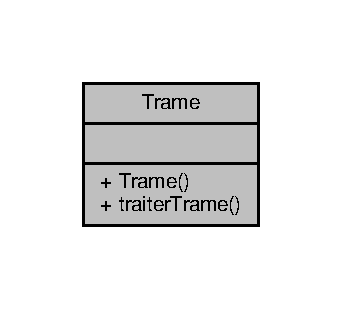
\includegraphics[width=164pt]{class_trame__coll__graph}
\end{center}
\end{figure}
\subsubsection*{Connecteurs publics}
\begin{DoxyCompactItemize}
\item 
void \hyperlink{class_trame_af6397dc6452101d13d8cccd53205a937}{traiter\+Trame} (Q\+String)
\begin{DoxyCompactList}\small\item\em Slot qui vas traiter la trame. \end{DoxyCompactList}\end{DoxyCompactItemize}
\subsubsection*{Signaux}
\begin{DoxyCompactItemize}
\item 
void \hyperlink{class_trame_ae7f5191744273a6bb4347aa477bdfaff}{donnees\+Trottinette} (Q\+String, Q\+String, Q\+String, Q\+String)
\begin{DoxyCompactList}\small\item\em Signal émettant les données de fonctionnement de la trottinette. \end{DoxyCompactList}\item 
void \hyperlink{class_trame_a8286aea8fb78e2e148f3f0dc35e8b079}{risque\+De\+Chute} (Q\+String)
\end{DoxyCompactItemize}
\subsubsection*{Fonctions membres publiques}
\begin{DoxyCompactItemize}
\item 
\hyperlink{class_trame_ae40bffc8a1e3f6ad9dec4710b673a57a}{Trame} (Q\+Object $\ast$parent=nullptr)
\begin{DoxyCompactList}\small\item\em Constructeur de la classe \hyperlink{class_trame}{Trame}. \end{DoxyCompactList}\end{DoxyCompactItemize}


\subsubsection{Description détaillée}
\begin{DoxyAuthor}{Auteur}
Somphon Sy
\end{DoxyAuthor}
\begin{DoxyVersion}{Version}
1.\+1 
\end{DoxyVersion}


\subsubsection{Documentation des constructeurs et destructeur}
\mbox{\Hypertarget{class_trame_ae40bffc8a1e3f6ad9dec4710b673a57a}\label{class_trame_ae40bffc8a1e3f6ad9dec4710b673a57a}} 
\index{Trame@{Trame}!Trame@{Trame}}
\index{Trame@{Trame}!Trame@{Trame}}
\paragraph{\texorpdfstring{Trame()}{Trame()}}
{\footnotesize\ttfamily Trame\+::\+Trame (\begin{DoxyParamCaption}\item[{Q\+Object $\ast$}]{parent = {\ttfamily nullptr} }\end{DoxyParamCaption})\hspace{0.3cm}{\ttfamily [explicit]}}


\begin{DoxyParams}{Paramètres}
{\em parent} & Q\+Object Adresse de l\textquotesingle{}objet Qt parent \\
\hline
\end{DoxyParams}

\begin{DoxyCode}
00025                             : QObject(parent)
00026 \{
00027 
00028 \}
\end{DoxyCode}


\subsubsection{Documentation des fonctions membres}
\mbox{\Hypertarget{class_trame_ae7f5191744273a6bb4347aa477bdfaff}\label{class_trame_ae7f5191744273a6bb4347aa477bdfaff}} 
\index{Trame@{Trame}!donnees\+Trottinette@{donnees\+Trottinette}}
\index{donnees\+Trottinette@{donnees\+Trottinette}!Trame@{Trame}}
\paragraph{\texorpdfstring{donnees\+Trottinette}{donneesTrottinette}}
{\footnotesize\ttfamily void Trame\+::donnees\+Trottinette (\begin{DoxyParamCaption}\item[{Q\+String}]{,  }\item[{Q\+String}]{,  }\item[{Q\+String}]{,  }\item[{Q\+String}]{ }\end{DoxyParamCaption})\hspace{0.3cm}{\ttfamily [signal]}}



Référencé par \hyperlink{class_trame_af6397dc6452101d13d8cccd53205a937}{traiter\+Trame()}.

\mbox{\Hypertarget{class_trame_a8286aea8fb78e2e148f3f0dc35e8b079}\label{class_trame_a8286aea8fb78e2e148f3f0dc35e8b079}} 
\index{Trame@{Trame}!risque\+De\+Chute@{risque\+De\+Chute}}
\index{risque\+De\+Chute@{risque\+De\+Chute}!Trame@{Trame}}
\paragraph{\texorpdfstring{risque\+De\+Chute}{risqueDeChute}}
{\footnotesize\ttfamily void Trame\+::risque\+De\+Chute (\begin{DoxyParamCaption}\item[{Q\+String}]{ }\end{DoxyParamCaption})\hspace{0.3cm}{\ttfamily [signal]}}



Référencé par \hyperlink{class_trame_af6397dc6452101d13d8cccd53205a937}{traiter\+Trame()}.

\mbox{\Hypertarget{class_trame_af6397dc6452101d13d8cccd53205a937}\label{class_trame_af6397dc6452101d13d8cccd53205a937}} 
\index{Trame@{Trame}!traiter\+Trame@{traiter\+Trame}}
\index{traiter\+Trame@{traiter\+Trame}!Trame@{Trame}}
\paragraph{\texorpdfstring{traiter\+Trame}{traiterTrame}}
{\footnotesize\ttfamily void Trame\+::traiter\+Trame (\begin{DoxyParamCaption}\item[{Q\+String}]{trame }\end{DoxyParamCaption})\hspace{0.3cm}{\ttfamily [slot]}}

Slot qui vas traiter la trame vas emettre le signal contenant les données de fonctionnement de la trottinette.


\begin{DoxyParams}{Paramètres}
{\em trame} & Q\+String trame émise par la trottinette \\
\hline
\end{DoxyParams}


Références \hyperlink{class_trame_ae7f5191744273a6bb4347aa477bdfaff}{donnees\+Trottinette()}, et \hyperlink{class_trame_a8286aea8fb78e2e148f3f0dc35e8b079}{risque\+De\+Chute()}.


\begin{DoxyCode}
00039 \{
00040     QString vitesse;
00041     QString inclinaison;
00042     QString batterie;
00043     QString distanceParcourue ;
00044     QString indicateurRisqueDeChute;
00045     qDebug() << Q\_FUNC\_INFO << trame;
00046     \textcolor{keywordflow}{if}(trame.startsWith(\textcolor{stringliteral}{"TEC"}))
00047     \{
00048         inclinaison = trame.section(\textcolor{charliteral}{';'},1,1);
00049         batterie = trame.section(\textcolor{charliteral}{';'},2,2);
00050         vitesse = trame.section(\textcolor{charliteral}{';'},3,3);
00051         distanceParcourue = trame.section(\textcolor{charliteral}{';'},4,4);
00052         indicateurRisqueDeChute=trame.section(\textcolor{stringliteral}{";"},5,5);
00053 
00054         qDebug()<< \textcolor{stringliteral}{"La vitesse est de : "} << vitesse << \textcolor{stringliteral}{"L'inclinaison est de : "} << inclinaison;
00055         qDebug()<< \textcolor{stringliteral}{"La batterie est de : "} << batterie << \textcolor{stringliteral}{"La distance parcourue est de : "} << 
      distanceParcourue;
00056         qDebug()<< \textcolor{stringliteral}{"Risque de chute: "} << indicateurRisqueDeChute ;
00057         emit \hyperlink{class_trame_ae7f5191744273a6bb4347aa477bdfaff}{donneesTrottinette}(vitesse , inclinaison,batterie , distanceParcourue);
00058         emit \hyperlink{class_trame_a8286aea8fb78e2e148f3f0dc35e8b079}{risqueDeChute}(indicateurRisqueDeChute);
00059     \}
00060 \}
\end{DoxyCode}


La documentation de cette classe a été générée à partir des fichiers suivants \+:\begin{DoxyCompactItemize}
\item 
\hyperlink{trame_8h}{trame.\+h}\item 
\hyperlink{trame_8cpp}{trame.\+cpp}\end{DoxyCompactItemize}

\hypertarget{class_trottinette}{}\subsection{Référence de la classe Trottinette}
\label{class_trottinette}\index{Trottinette@{Trottinette}}


Déclaration de la classe \hyperlink{class_trottinette}{Trottinette}.  




{\ttfamily \#include $<$trottinette.\+h$>$}



Graphe de collaboration de Trottinette\+:\nopagebreak
\begin{figure}[H]
\begin{center}
\leavevmode
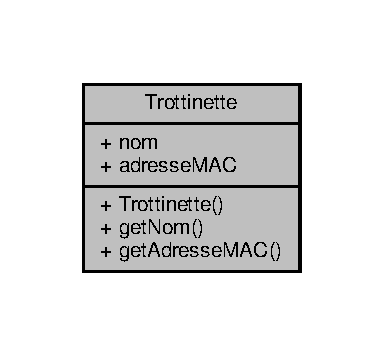
\includegraphics[width=184pt]{class_trottinette__coll__graph}
\end{center}
\end{figure}
\subsubsection*{Signaux}
\begin{DoxyCompactItemize}
\item 
void \hyperlink{class_trottinette_a44ae1514740ee0a1a55a9dab39c37aaf}{peripherique\+Changed} ()
\begin{DoxyCompactList}\small\item\em les attributs du périphériques ont changé \end{DoxyCompactList}\end{DoxyCompactItemize}
\subsubsection*{Fonctions membres publiques}
\begin{DoxyCompactItemize}
\item 
\hyperlink{class_trottinette_ab3c84f129214e5dcf8f9d11cf7f3e3e0}{Trottinette} (Q\+String \hyperlink{class_trottinette_aab7d536bd21b3dbf0b9cca5508db40ab}{nom}, Q\+String \hyperlink{class_trottinette_acd01acc5c1cbf23b9b527401282f1136}{adresse\+M\+AC}, Q\+Object $\ast$parent=nullptr)
\begin{DoxyCompactList}\small\item\em Constructeur de la classe \hyperlink{class_trottinette}{Trottinette}. \end{DoxyCompactList}\item 
Q\+String \hyperlink{class_trottinette_a9b191a43bacb534dca0727aedd3076cd}{get\+Nom} ()
\begin{DoxyCompactList}\small\item\em Retourne le nom de la trottinette. \end{DoxyCompactList}\item 
Q\+String \hyperlink{class_trottinette_a4d319bfda23b3d871b62e3e910cc204d}{get\+Adresse\+M\+AC} ()
\begin{DoxyCompactList}\small\item\em Retourne l\textquotesingle{}adresse M\+AC de la trottinette. \end{DoxyCompactList}\end{DoxyCompactItemize}
\subsubsection*{Propriétés}
\begin{DoxyCompactItemize}
\item 
Q\+String \hyperlink{class_trottinette_aab7d536bd21b3dbf0b9cca5508db40ab}{nom}
\begin{DoxyCompactList}\small\item\em nom du périphérique Bluetooth \end{DoxyCompactList}\item 
Q\+String \hyperlink{class_trottinette_acd01acc5c1cbf23b9b527401282f1136}{adresse\+M\+AC}
\begin{DoxyCompactList}\small\item\em adresse M\+AC du périphérique Bluetooth \end{DoxyCompactList}\end{DoxyCompactItemize}


\subsubsection{Description détaillée}
\begin{DoxyAuthor}{Auteur}
Somphon Sy
\end{DoxyAuthor}
\begin{DoxyVersion}{Version}
1.\+1 
\end{DoxyVersion}


\subsubsection{Documentation des constructeurs et destructeur}
\mbox{\Hypertarget{class_trottinette_ab3c84f129214e5dcf8f9d11cf7f3e3e0}\label{class_trottinette_ab3c84f129214e5dcf8f9d11cf7f3e3e0}} 
\index{Trottinette@{Trottinette}!Trottinette@{Trottinette}}
\index{Trottinette@{Trottinette}!Trottinette@{Trottinette}}
\paragraph{\texorpdfstring{Trottinette()}{Trottinette()}}
{\footnotesize\ttfamily Trottinette\+::\+Trottinette (\begin{DoxyParamCaption}\item[{Q\+String}]{nom,  }\item[{Q\+String}]{adresse\+M\+AC,  }\item[{Q\+Object $\ast$}]{parent = {\ttfamily nullptr} }\end{DoxyParamCaption})\hspace{0.3cm}{\ttfamily [explicit]}}


\begin{DoxyParams}{Paramètres}
{\em nom} & Q\+String nom \\
\hline
{\em adresse\+M\+AC} & Q\+String Adresse M\+AC \\
\hline
{\em parent} & Q\+Object Adresse de l\textquotesingle{}objet Qt parent \\
\hline
\end{DoxyParams}

\begin{DoxyCode}
00025                                                                           : QObject(parent) , 
      \hyperlink{class_trottinette_aab7d536bd21b3dbf0b9cca5508db40ab}{nom}(\hyperlink{class_trottinette_aab7d536bd21b3dbf0b9cca5508db40ab}{nom}) , \hyperlink{class_trottinette_acd01acc5c1cbf23b9b527401282f1136}{adresseMAC}(\hyperlink{class_trottinette_acd01acc5c1cbf23b9b527401282f1136}{adresseMAC})
00026 \{
00027 
00028 \}
\end{DoxyCode}


\subsubsection{Documentation des fonctions membres}
\mbox{\Hypertarget{class_trottinette_a4d319bfda23b3d871b62e3e910cc204d}\label{class_trottinette_a4d319bfda23b3d871b62e3e910cc204d}} 
\index{Trottinette@{Trottinette}!get\+Adresse\+M\+AC@{get\+Adresse\+M\+AC}}
\index{get\+Adresse\+M\+AC@{get\+Adresse\+M\+AC}!Trottinette@{Trottinette}}
\paragraph{\texorpdfstring{get\+Adresse\+M\+A\+C()}{getAdresseMAC()}}
{\footnotesize\ttfamily Q\+String Trottinette\+::get\+Adresse\+M\+AC (\begin{DoxyParamCaption}{ }\end{DoxyParamCaption})}

Accesseur de l\textquotesingle{}attribut adresse\+M\+AC.

\begin{DoxyReturn}{Renvoie}
Q\+String adresse M\+AC du périphérique Bluetooth 
\end{DoxyReturn}


Références \hyperlink{class_trottinette_acd01acc5c1cbf23b9b527401282f1136}{adresse\+M\+AC}.



Référencé par \hyperlink{class_peripherique_local_a465658a204541e309f2647d473f658d8}{Peripherique\+Local\+::get\+Trottinette\+Adresse\+Mac()}.


\begin{DoxyCode}
00050 \{
00051     \textcolor{keywordflow}{return} \hyperlink{class_trottinette_acd01acc5c1cbf23b9b527401282f1136}{adresseMAC};
00052 \}
\end{DoxyCode}
\mbox{\Hypertarget{class_trottinette_a9b191a43bacb534dca0727aedd3076cd}\label{class_trottinette_a9b191a43bacb534dca0727aedd3076cd}} 
\index{Trottinette@{Trottinette}!get\+Nom@{get\+Nom}}
\index{get\+Nom@{get\+Nom}!Trottinette@{Trottinette}}
\paragraph{\texorpdfstring{get\+Nom()}{getNom()}}
{\footnotesize\ttfamily Q\+String Trottinette\+::get\+Nom (\begin{DoxyParamCaption}{ }\end{DoxyParamCaption})}

Accesseur de l\textquotesingle{}attribut nom.

Accesseur de l\textquotesingle{}attribut M\+AC.

\begin{DoxyReturn}{Renvoie}
Q\+String M\+AC du périphérique local

Q\+String nom du périphérique Bluetooth 
\end{DoxyReturn}


Références \hyperlink{class_trottinette_aab7d536bd21b3dbf0b9cca5508db40ab}{nom}.



Référencé par \hyperlink{class_peripherique_local_ac81a942b4d1d9e848649073c53ed6917}{Peripherique\+Local\+::get\+Trottinette\+Nom()}.


\begin{DoxyCode}
00038 \{
00039     \textcolor{keywordflow}{return} \hyperlink{class_trottinette_aab7d536bd21b3dbf0b9cca5508db40ab}{nom};
00040 \}
\end{DoxyCode}
\mbox{\Hypertarget{class_trottinette_a44ae1514740ee0a1a55a9dab39c37aaf}\label{class_trottinette_a44ae1514740ee0a1a55a9dab39c37aaf}} 
\index{Trottinette@{Trottinette}!peripherique\+Changed@{peripherique\+Changed}}
\index{peripherique\+Changed@{peripherique\+Changed}!Trottinette@{Trottinette}}
\paragraph{\texorpdfstring{peripherique\+Changed}{peripheriqueChanged}}
{\footnotesize\ttfamily void Trottinette\+::peripherique\+Changed (\begin{DoxyParamCaption}{ }\end{DoxyParamCaption})\hspace{0.3cm}{\ttfamily [signal]}}



\subsubsection{Documentation des propriétés}
\mbox{\Hypertarget{class_trottinette_acd01acc5c1cbf23b9b527401282f1136}\label{class_trottinette_acd01acc5c1cbf23b9b527401282f1136}} 
\index{Trottinette@{Trottinette}!adresse\+M\+AC@{adresse\+M\+AC}}
\index{adresse\+M\+AC@{adresse\+M\+AC}!Trottinette@{Trottinette}}
\paragraph{\texorpdfstring{adresse\+M\+AC}{adresseMAC}}
{\footnotesize\ttfamily Q\+String Trottinette\+::adresse\+M\+AC\hspace{0.3cm}{\ttfamily [read]}}



Référencé par \hyperlink{class_trottinette_a4d319bfda23b3d871b62e3e910cc204d}{get\+Adresse\+M\+A\+C()}.

\mbox{\Hypertarget{class_trottinette_aab7d536bd21b3dbf0b9cca5508db40ab}\label{class_trottinette_aab7d536bd21b3dbf0b9cca5508db40ab}} 
\index{Trottinette@{Trottinette}!nom@{nom}}
\index{nom@{nom}!Trottinette@{Trottinette}}
\paragraph{\texorpdfstring{nom}{nom}}
{\footnotesize\ttfamily Q\+String Trottinette\+::nom\hspace{0.3cm}{\ttfamily [read]}}



Référencé par \hyperlink{class_trottinette_a9b191a43bacb534dca0727aedd3076cd}{get\+Nom()}.



La documentation de cette classe a été générée à partir des fichiers suivants \+:\begin{DoxyCompactItemize}
\item 
\hyperlink{trottinette_8h}{trottinette.\+h}\item 
\hyperlink{peripheriquelocal_8cpp}{peripheriquelocal.\+cpp}\item 
\hyperlink{trottinette_8cpp}{trottinette.\+cpp}\end{DoxyCompactItemize}

\section{Documentation des fichiers}
\hypertarget{_application_8qml}{}\subsection{Référence du fichier Application.\+qml}
\label{_application_8qml}\index{Application.\+qml@{Application.\+qml}}


Définition de la fenêtre principale de l\textquotesingle{}application terminal mobile.  


\subsubsection*{Classes}
\begin{DoxyCompactItemize}
\item 
class \hyperlink{class_application}{Application}
\begin{DoxyCompactList}\small\item\em La fenêtre principale de l\textquotesingle{}application terminal mobile. \end{DoxyCompactList}\end{DoxyCompactItemize}


\subsubsection{Description détaillée}
\begin{DoxyAuthor}{Auteur}
Somphon Sy
\end{DoxyAuthor}
\begin{DoxyVersion}{Version}
1.\+1 
\end{DoxyVersion}

\hypertarget{_changelog_8md}{}\subsection{Référence du fichier Changelog.\+md}
\label{_changelog_8md}\index{Changelog.\+md@{Changelog.\+md}}

\hypertarget{chronometreutilisation_8cpp}{}\subsection{Référence du fichier chronometreutilisation.\+cpp}
\label{chronometreutilisation_8cpp}\index{chronometreutilisation.\+cpp@{chronometreutilisation.\+cpp}}


Définition de la classe \hyperlink{class_chronometre_utilisation}{Chronometre\+Utilisation}.  


{\ttfamily \#include \char`\"{}chronometreutilisation.\+h\char`\"{}}\newline
{\ttfamily \#include $<$Q\+Debug$>$}\newline


\subsubsection{Description détaillée}
\begin{DoxyAuthor}{Auteur}
Somphon Sy
\end{DoxyAuthor}
\begin{DoxyVersion}{Version}
1.\+1 
\end{DoxyVersion}

\hypertarget{chronometreutilisation_8h}{}\subsection{Référence du fichier chronometreutilisation.\+h}
\label{chronometreutilisation_8h}\index{chronometreutilisation.\+h@{chronometreutilisation.\+h}}


Déclaration de la classe \hyperlink{class_chronometre_utilisation}{Chronometre\+Utilisation}.  


{\ttfamily \#include $<$Q\+Object$>$}\newline
{\ttfamily \#include $<$Q\+Timer$>$}\newline
\subsubsection*{Classes}
\begin{DoxyCompactItemize}
\item 
class \hyperlink{class_chronometre_utilisation}{Chronometre\+Utilisation}
\begin{DoxyCompactList}\small\item\em Déclaration de la classe \hyperlink{class_chronometre_utilisation}{Chronometre\+Utilisation}. \end{DoxyCompactList}\end{DoxyCompactItemize}
\subsubsection*{Macros}
\begin{DoxyCompactItemize}
\item 
\#define \hyperlink{chronometreutilisation_8h_ad0750d12e2f5f404ec458d4066a53fa4}{P\+E\+R\+I\+O\+DE}~100
\end{DoxyCompactItemize}


\subsubsection{Description détaillée}
\begin{DoxyAuthor}{Auteur}
Somphon Sy
\end{DoxyAuthor}
\begin{DoxyVersion}{Version}
1.\+1 
\end{DoxyVersion}


\subsubsection{Documentation des macros}
\mbox{\Hypertarget{chronometreutilisation_8h_ad0750d12e2f5f404ec458d4066a53fa4}\label{chronometreutilisation_8h_ad0750d12e2f5f404ec458d4066a53fa4}} 
\index{chronometreutilisation.\+h@{chronometreutilisation.\+h}!P\+E\+R\+I\+O\+DE@{P\+E\+R\+I\+O\+DE}}
\index{P\+E\+R\+I\+O\+DE@{P\+E\+R\+I\+O\+DE}!chronometreutilisation.\+h@{chronometreutilisation.\+h}}
\paragraph{\texorpdfstring{P\+E\+R\+I\+O\+DE}{PERIODE}}
{\footnotesize\ttfamily \#define P\+E\+R\+I\+O\+DE~100}



Référencé par \hyperlink{class_peripherique_local_ae4f8521445a9dc3a51ff116e1f6597d7}{Peripherique\+Local\+::regler\+Chrono()}.


\hypertarget{main_8cpp}{}\subsection{Référence du fichier main.\+cpp}
\label{main_8cpp}\index{main.\+cpp@{main.\+cpp}}


Programme principal.  


{\ttfamily \#include $<$Q\+Gui\+Application$>$}\newline
{\ttfamily \#include $<$Q\+Qml\+Application\+Engine$>$}\newline
{\ttfamily \#include $<$Q\+Qml\+Context$>$}\newline
{\ttfamily \#include $<$Q\+Quick\+Style$>$}\newline
{\ttfamily \#include $<$Q\+Icon$>$}\newline
{\ttfamily \#include $<$Q\+Debug$>$}\newline
{\ttfamily \#include \char`\"{}peripheriquelocal.\+h\char`\"{}}\newline
\subsubsection*{Fonctions}
\begin{DoxyCompactItemize}
\item 
int \hyperlink{main_8cpp_ae0665038b72011f5c680c660fcb59459}{main} (int argc, char $\ast$argv\mbox{[}$\,$\mbox{]})
\end{DoxyCompactItemize}


\subsubsection{Description détaillée}
Crée et affiche la fenêtre principale de l\textquotesingle{}application

\begin{DoxyAuthor}{Auteur}
Somphon Sy
\end{DoxyAuthor}
\begin{DoxyVersion}{Version}
1.\+1 
\end{DoxyVersion}


\subsubsection{Documentation des fonctions}
\mbox{\Hypertarget{main_8cpp_ae0665038b72011f5c680c660fcb59459}\label{main_8cpp_ae0665038b72011f5c680c660fcb59459}} 
\index{main.\+cpp@{main.\+cpp}!main@{main}}
\index{main@{main}!main.\+cpp@{main.\+cpp}}
\paragraph{\texorpdfstring{main()}{main()}}
{\footnotesize\ttfamily main (\begin{DoxyParamCaption}\item[{int}]{argc,  }\item[{char $\ast$}]{argv\mbox{[}$\,$\mbox{]} }\end{DoxyParamCaption})}


\begin{DoxyParams}{Paramètres}
{\em argc} & \\
\hline
{\em argv\mbox{[}$\,$\mbox{]}} & \\
\hline
\end{DoxyParams}
\begin{DoxyReturn}{Renvoie}
int 
\end{DoxyReturn}

\begin{DoxyCode}
00028 \{
00029     QCoreApplication::setAttribute(Qt::AA\_EnableHighDpiScaling);
00030     QGuiApplication app(argc, argv);
00031     QQmlApplicationEngine engine;
00032 
00033     QQuickStyle::setStyle(\textcolor{stringliteral}{"Material"}); \textcolor{comment}{// ("Default", "Fusion", "Imagine", "Material", "Universal")}
00034     QIcon::setThemeName(\textcolor{stringliteral}{"mytheme"});
00035 
00036     engine.rootContext()->setContextProperty(\textcolor{stringliteral}{"peripheriqueLocal"}, \textcolor{keyword}{new} 
      \hyperlink{class_peripherique_local}{PeripheriqueLocal}());
00037     engine.load(QUrl(QStringLiteral(\textcolor{stringliteral}{"qrc:/Application.qml"})));
00038     \textcolor{keywordflow}{if} (engine.rootObjects().isEmpty())
00039         \textcolor{keywordflow}{return} -1;
00040 
00041     \textcolor{keywordflow}{return} app.exec();
00042 \}
\end{DoxyCode}

\hypertarget{_page_accueil_8qml}{}\subsection{Référence du fichier Page\+Accueil.\+qml}
\label{_page_accueil_8qml}\index{Page\+Accueil.\+qml@{Page\+Accueil.\+qml}}


Définition de la page d\textquotesingle{}accueil de l\textquotesingle{}application.  


\subsubsection*{Classes}
\begin{DoxyCompactItemize}
\item 
class \hyperlink{class_page_accueil}{Page\+Accueil}
\begin{DoxyCompactList}\small\item\em La page d\textquotesingle{}accueil de l\textquotesingle{}application. \end{DoxyCompactList}\end{DoxyCompactItemize}


\subsubsection{Description détaillée}
\begin{DoxyAuthor}{Auteur}
Somphon Sy
\end{DoxyAuthor}
\begin{DoxyVersion}{Version}
1.\+1 
\end{DoxyVersion}

\hypertarget{_page_carte_8qml}{}\subsection{Référence du fichier Page\+Carte.\+qml}
\label{_page_carte_8qml}\index{Page\+Carte.\+qml@{Page\+Carte.\+qml}}


Définition de la page de navigation (Carte et/ou Télémétrie)  


\subsubsection*{Classes}
\begin{DoxyCompactItemize}
\item 
class \hyperlink{class_page_carte}{Page\+Carte}
\begin{DoxyCompactList}\small\item\em La page de navigation (Carte et/ou Télémétrie) \end{DoxyCompactList}\end{DoxyCompactItemize}


\subsubsection{Description détaillée}
\begin{DoxyAuthor}{Auteur}
Somphon Sy
\end{DoxyAuthor}
\begin{DoxyVersion}{Version}
1.\+1 
\end{DoxyVersion}

\hypertarget{peripheriquelocal_8cpp}{}\subsection{Référence du fichier peripheriquelocal.\+cpp}
\label{peripheriquelocal_8cpp}\index{peripheriquelocal.\+cpp@{peripheriquelocal.\+cpp}}


Définition de la classe \hyperlink{class_peripherique_local}{Peripherique\+Local}.  


{\ttfamily \#include \char`\"{}peripheriquelocal.\+h\char`\"{}}\newline
{\ttfamily \#include \char`\"{}trottinette.\+h\char`\"{}}\newline
{\ttfamily \#include $<$unistd.\+h$>$}\newline
{\ttfamily \#include $<$Q\+Bluetooth\+Device\+Info$>$}\newline
{\ttfamily \#include $<$Q\+Byte\+Array$>$}\newline
{\ttfamily \#include $<$Q\+Debug$>$}\newline
{\ttfamily \#include $<$Qt\+Endian$>$}\newline
{\ttfamily \#include \char`\"{}trame.\+h\char`\"{}}\newline


\subsubsection{Description détaillée}
\begin{DoxyAuthor}{Auteur}
Somphon Sy
\end{DoxyAuthor}
\begin{DoxyVersion}{Version}
1.\+1 
\end{DoxyVersion}

\hypertarget{peripheriquelocal_8h}{}\subsection{Référence du fichier peripheriquelocal.\+h}
\label{peripheriquelocal_8h}\index{peripheriquelocal.\+h@{peripheriquelocal.\+h}}


Déclaration de la classe \hyperlink{class_peripherique_local}{Peripherique\+Local}.  


{\ttfamily \#include $<$Q\+Object$>$}\newline
{\ttfamily \#include $<$Q\+Bluetooth\+Local\+Device$>$}\newline
{\ttfamily \#include $<$Q\+Bluetooth\+Address$>$}\newline
{\ttfamily \#include $<$Q\+Bluetooth\+Uuid$>$}\newline
{\ttfamily \#include $<$Q\+Bluetooth\+Socket$>$}\newline
{\ttfamily \#include $<$Q\+Bluetooth\+Device\+Info$>$}\newline
{\ttfamily \#include $<$Q\+Bluetooth\+Service\+Info$>$}\newline
{\ttfamily \#include $<$Q\+Bluetooth\+Device\+Discovery\+Agent$>$}\newline
{\ttfamily \#include \char`\"{}trottinette.\+h\char`\"{}}\newline
{\ttfamily \#include \char`\"{}trame.\+h\char`\"{}}\newline
{\ttfamily \#include \char`\"{}chronometreutilisation.\+h\char`\"{}}\newline
\subsubsection*{Classes}
\begin{DoxyCompactItemize}
\item 
class \hyperlink{class_peripherique_local}{Peripherique\+Local}
\begin{DoxyCompactList}\small\item\em Déclaration de la classe \hyperlink{class_peripherique_local}{Peripherique\+Local}. \end{DoxyCompactList}\end{DoxyCompactItemize}


\subsubsection{Description détaillée}
\begin{DoxyAuthor}{Auteur}
Somphon Sy
\end{DoxyAuthor}
\begin{DoxyVersion}{Version}
1.\+1 
\end{DoxyVersion}

\hypertarget{_r_e_a_d_m_e_8md}{}\subsection{Référence du fichier R\+E\+A\+D\+M\+E.\+md}
\label{_r_e_a_d_m_e_8md}\index{R\+E\+A\+D\+M\+E.\+md@{R\+E\+A\+D\+M\+E.\+md}}

\hypertarget{trame_8cpp}{}\subsection{Référence du fichier trame.\+cpp}
\label{trame_8cpp}\index{trame.\+cpp@{trame.\+cpp}}


Définition de la classe \hyperlink{class_trame}{Trame}.  


{\ttfamily \#include \char`\"{}trame.\+h\char`\"{}}\newline
{\ttfamily \#include $<$Q\+Debug$>$}\newline


\subsubsection{Description détaillée}
\begin{DoxyAuthor}{Auteur}
Somphon Sy
\end{DoxyAuthor}
\begin{DoxyVersion}{Version}
1.\+1 
\end{DoxyVersion}

\hypertarget{trame_8h}{}\subsection{Référence du fichier trame.\+h}
\label{trame_8h}\index{trame.\+h@{trame.\+h}}


Déclaration de la classe \hyperlink{class_trame}{Trame}.  


{\ttfamily \#include $<$Q\+Object$>$}\newline
\subsubsection*{Classes}
\begin{DoxyCompactItemize}
\item 
class \hyperlink{class_trame}{Trame}
\begin{DoxyCompactList}\small\item\em Déclaration de la classe \hyperlink{class_trame}{Trame}. \end{DoxyCompactList}\end{DoxyCompactItemize}


\subsubsection{Description détaillée}
\begin{DoxyAuthor}{Auteur}
Somphon Sy
\end{DoxyAuthor}
\begin{DoxyVersion}{Version}
1.\+1 
\end{DoxyVersion}

\hypertarget{trottinette_8cpp}{}\subsection{Référence du fichier trottinette.\+cpp}
\label{trottinette_8cpp}\index{trottinette.\+cpp@{trottinette.\+cpp}}


Définition de la classe \hyperlink{class_trottinette}{Trottinette}.  


{\ttfamily \#include \char`\"{}trottinette.\+h\char`\"{}}\newline
{\ttfamily \#include \char`\"{}peripheriquelocal.\+h\char`\"{}}\newline


\subsubsection{Description détaillée}
\begin{DoxyAuthor}{Auteur}
Somphon Sy
\end{DoxyAuthor}
\begin{DoxyVersion}{Version}
1.\+1 
\end{DoxyVersion}

\hypertarget{trottinette_8h}{}\subsection{Référence du fichier trottinette.\+h}
\label{trottinette_8h}\index{trottinette.\+h@{trottinette.\+h}}


Déclaration de la classe \hyperlink{class_trottinette}{Trottinette}.  


{\ttfamily \#include $<$Q\+Object$>$}\newline
\subsubsection*{Classes}
\begin{DoxyCompactItemize}
\item 
class \hyperlink{class_trottinette}{Trottinette}
\begin{DoxyCompactList}\small\item\em Déclaration de la classe \hyperlink{class_trottinette}{Trottinette}. \end{DoxyCompactList}\end{DoxyCompactItemize}


\subsubsection{Description détaillée}
\begin{DoxyAuthor}{Auteur}
Somphon Sy
\end{DoxyAuthor}
\begin{DoxyVersion}{Version}
1.\+1 
\end{DoxyVersion}

%--- End generated contents ---

% Index
\newpage
\phantomsection
\clearemptydoublepage
\addcontentsline{toc}{section}{Index}
\printindex

\end{document}
